\documentclass[twoside]{book}

% Packages required by doxygen
\usepackage{fixltx2e}
\usepackage{calc}
\usepackage{doxygen}
\usepackage[export]{adjustbox} % also loads graphicx
\usepackage{graphicx}
\usepackage[utf8]{inputenc}
\usepackage{makeidx}
\usepackage{multicol}
\usepackage{multirow}
\PassOptionsToPackage{warn}{textcomp}
\usepackage{textcomp}
\usepackage[nointegrals]{wasysym}
\usepackage[table]{xcolor}

% Font selection
\usepackage[T1]{fontenc}
\usepackage[scaled=.90]{helvet}
\usepackage{courier}
\usepackage{amssymb}
\usepackage{sectsty}
\renewcommand{\familydefault}{\sfdefault}
\allsectionsfont{%
  \fontseries{bc}\selectfont%
  \color{darkgray}%
}
\renewcommand{\DoxyLabelFont}{%
  \fontseries{bc}\selectfont%
  \color{darkgray}%
}
\newcommand{\+}{\discretionary{\mbox{\scriptsize$\hookleftarrow$}}{}{}}

% Page & text layout
\usepackage{geometry}
\geometry{%
  a4paper,%
  top=2.5cm,%
  bottom=2.5cm,%
  left=2.5cm,%
  right=2.5cm%
}
\tolerance=750
\hfuzz=15pt
\hbadness=750
\setlength{\emergencystretch}{15pt}
\setlength{\parindent}{0cm}
\setlength{\parskip}{3ex plus 2ex minus 2ex}
\makeatletter
\renewcommand{\paragraph}{%
  \@startsection{paragraph}{4}{0ex}{-1.0ex}{1.0ex}{%
    \normalfont\normalsize\bfseries\SS@parafont%
  }%
}
\renewcommand{\subparagraph}{%
  \@startsection{subparagraph}{5}{0ex}{-1.0ex}{1.0ex}{%
    \normalfont\normalsize\bfseries\SS@subparafont%
  }%
}
\makeatother

% Headers & footers
\usepackage{fancyhdr}
\pagestyle{fancyplain}
\fancyhead[LE]{\fancyplain{}{\bfseries\thepage}}
\fancyhead[CE]{\fancyplain{}{}}
\fancyhead[RE]{\fancyplain{}{\bfseries\leftmark}}
\fancyhead[LO]{\fancyplain{}{\bfseries\rightmark}}
\fancyhead[CO]{\fancyplain{}{}}
\fancyhead[RO]{\fancyplain{}{\bfseries\thepage}}
\fancyfoot[LE]{\fancyplain{}{}}
\fancyfoot[CE]{\fancyplain{}{}}
\fancyfoot[RE]{\fancyplain{}{\bfseries\scriptsize Generated by Doxygen }}
\fancyfoot[LO]{\fancyplain{}{\bfseries\scriptsize Generated by Doxygen }}
\fancyfoot[CO]{\fancyplain{}{}}
\fancyfoot[RO]{\fancyplain{}{}}
\renewcommand{\footrulewidth}{0.4pt}
\renewcommand{\chaptermark}[1]{%
  \markboth{#1}{}%
}
\renewcommand{\sectionmark}[1]{%
  \markright{\thesection\ #1}%
}

% Indices & bibliography
\usepackage{natbib}
\usepackage[titles]{tocloft}
\setcounter{tocdepth}{3}
\setcounter{secnumdepth}{5}
\makeindex

% Hyperlinks (required, but should be loaded last)
\usepackage{ifpdf}
\ifpdf
  \usepackage[pdftex,pagebackref=true]{hyperref}
\else
  \usepackage[ps2pdf,pagebackref=true]{hyperref}
\fi
\hypersetup{%
  colorlinks=true,%
  linkcolor=blue,%
  citecolor=blue,%
  unicode%
}

% Custom commands
\newcommand{\clearemptydoublepage}{%
  \newpage{\pagestyle{empty}\cleardoublepage}%
}

\usepackage{caption}
\captionsetup{labelsep=space,justification=centering,font={bf},singlelinecheck=off,skip=4pt,position=top}

%===== C O N T E N T S =====

\begin{document}

% Titlepage & ToC
\hypersetup{pageanchor=false,
             bookmarksnumbered=true,
             pdfencoding=unicode
            }
\pagenumbering{alph}
\begin{titlepage}
\vspace*{7cm}
\begin{center}%
{\Large ultra64 \\[1ex]\large 0.\+1 }\\
\vspace*{1cm}
{\large Generated by Doxygen 1.8.13}\\
\end{center}
\end{titlepage}
\clearemptydoublepage
\pagenumbering{roman}
\tableofcontents
\clearemptydoublepage
\pagenumbering{arabic}
\hypersetup{pageanchor=true}

%--- Begin generated contents ---
\chapter{ultra64}
\label{md__r_e_a_d_m_e}
\Hypertarget{md__r_e_a_d_m_e}
Nintendo 64 emulator 
\chapter{Namespace Index}
\section{Namespace List}
Here is a list of all namespaces with brief descriptions\+:\begin{DoxyCompactList}
\item\contentsline{section}{\hyperlink{namespaceultra64}{ultra64} }{\pageref{namespaceultra64}}{}
\end{DoxyCompactList}

\chapter{Hierarchical Index}
\section{Class Hierarchy}
This inheritance list is sorted roughly, but not completely, alphabetically\+:\begin{DoxyCompactList}
\item \contentsline{section}{ultra64\+:\+:memory\+\_\+section}{\pageref{structultra64_1_1memory__section}}{}
\item \contentsline{section}{ultra64\+:\+:M\+MU}{\pageref{classultra64_1_1_m_m_u}}{}
\item \contentsline{section}{ultra64\+:\+:opcode\+\_\+t}{\pageref{classultra64_1_1opcode__t}}{}
\item \contentsline{section}{ultra64\+:\+:P\+I\+F\+\_\+\+R\+OM}{\pageref{classultra64_1_1_p_i_f___r_o_m}}{}
\item \contentsline{section}{ultra64\+:\+:r4300}{\pageref{classultra64_1_1r4300}}{}
\item \contentsline{section}{ultra64\+:\+:R\+OM}{\pageref{classultra64_1_1_r_o_m}}{}
\item \contentsline{section}{ultra64\+:\+:R\+O\+M\+\_\+header}{\pageref{structultra64_1_1_r_o_m__header}}{}
\item \contentsline{section}{ultra64\+:\+:rsp}{\pageref{classultra64_1_1rsp}}{}
\item wx\+App\begin{DoxyCompactList}
\item \contentsline{section}{wx\+Ultra64}{\pageref{classwx_ultra64}}{}
\end{DoxyCompactList}
\item wx\+Frame\begin{DoxyCompactList}
\item \contentsline{section}{Debugger\+Window}{\pageref{class_debugger_window}}{}
\item \contentsline{section}{Main\+Window}{\pageref{class_main_window}}{}
\item \contentsline{section}{Registers\+Window}{\pageref{class_registers_window}}{}
\end{DoxyCompactList}
\end{DoxyCompactList}

\chapter{Class Index}
\section{Class List}
Here are the classes, structs, unions and interfaces with brief descriptions\+:\begin{DoxyCompactList}
\item\contentsline{section}{\hyperlink{class_debugger_window}{Debugger\+Window} }{\pageref{class_debugger_window}}{}
\item\contentsline{section}{\hyperlink{class_main_window}{Main\+Window} }{\pageref{class_main_window}}{}
\item\contentsline{section}{\hyperlink{structultra64_1_1memory__section}{ultra64\+::memory\+\_\+section} }{\pageref{structultra64_1_1memory__section}}{}
\item\contentsline{section}{\hyperlink{classultra64_1_1_m_m_u}{ultra64\+::\+M\+MU} }{\pageref{classultra64_1_1_m_m_u}}{}
\item\contentsline{section}{\hyperlink{classultra64_1_1opcode__t}{ultra64\+::opcode\+\_\+t} }{\pageref{classultra64_1_1opcode__t}}{}
\item\contentsline{section}{\hyperlink{classultra64_1_1_p_i_f___r_o_m}{ultra64\+::\+P\+I\+F\+\_\+\+R\+OM} }{\pageref{classultra64_1_1_p_i_f___r_o_m}}{}
\item\contentsline{section}{\hyperlink{classultra64_1_1r4300}{ultra64\+::r4300} }{\pageref{classultra64_1_1r4300}}{}
\item\contentsline{section}{\hyperlink{class_registers_window}{Registers\+Window} }{\pageref{class_registers_window}}{}
\item\contentsline{section}{\hyperlink{classultra64_1_1_r_o_m}{ultra64\+::\+R\+OM} }{\pageref{classultra64_1_1_r_o_m}}{}
\item\contentsline{section}{\hyperlink{structultra64_1_1_r_o_m__header}{ultra64\+::\+R\+O\+M\+\_\+header} }{\pageref{structultra64_1_1_r_o_m__header}}{}
\item\contentsline{section}{\hyperlink{classultra64_1_1rsp}{ultra64\+::rsp} }{\pageref{classultra64_1_1rsp}}{}
\item\contentsline{section}{\hyperlink{classwx_ultra64}{wx\+Ultra64} }{\pageref{classwx_ultra64}}{}
\end{DoxyCompactList}

\chapter{File Index}
\section{File List}
Here is a list of all files with brief descriptions\+:\begin{DoxyCompactList}
\item\contentsline{section}{\hyperlink{config_8h}{config.\+h} }{\pageref{config_8h}}{}
\item\contentsline{section}{include/\hyperlink{memory_8h}{memory.\+h} }{\pageref{memory_8h}}{}
\item\contentsline{section}{include/\hyperlink{opcodes_8h}{opcodes.\+h} }{\pageref{opcodes_8h}}{}
\item\contentsline{section}{include/\hyperlink{pif__rom_8h}{pif\+\_\+rom.\+h} }{\pageref{pif__rom_8h}}{}
\item\contentsline{section}{include/\hyperlink{r4300_8h}{r4300.\+h} }{\pageref{r4300_8h}}{}
\item\contentsline{section}{include/\hyperlink{rom_8h}{rom.\+h} }{\pageref{rom_8h}}{}
\item\contentsline{section}{include/\hyperlink{rsp_8h}{rsp.\+h} }{\pageref{rsp_8h}}{}
\item\contentsline{section}{include/\hyperlink{ultra64_8h}{ultra64.\+h} }{\pageref{ultra64_8h}}{}
\item\contentsline{section}{src/\hyperlink{memory_8cpp}{memory.\+cpp} }{\pageref{memory_8cpp}}{}
\item\contentsline{section}{src/\hyperlink{pif__rom_8cpp}{pif\+\_\+rom.\+cpp} }{\pageref{pif__rom_8cpp}}{}
\item\contentsline{section}{src/\hyperlink{rom_8cpp}{rom.\+cpp} }{\pageref{rom_8cpp}}{}
\item\contentsline{section}{src/\hyperlink{ultra64_8cpp}{ultra64.\+cpp} }{\pageref{ultra64_8cpp}}{}
\item\contentsline{section}{src/r4300/\hyperlink{cp0_8cpp}{cp0.\+cpp} }{\pageref{cp0_8cpp}}{}
\item\contentsline{section}{src/r4300/\hyperlink{r4300_8cpp}{r4300.\+cpp} }{\pageref{r4300_8cpp}}{}
\item\contentsline{section}{src/r4300/\hyperlink{special_8cpp}{special.\+cpp} }{\pageref{special_8cpp}}{}
\item\contentsline{section}{src/rcp/\hyperlink{rsp_8cpp}{rsp.\+cpp} }{\pageref{rsp_8cpp}}{}
\end{DoxyCompactList}

\chapter{Namespace Documentation}
\hypertarget{namespaceultra64}{}\section{ultra64 Namespace Reference}
\label{namespaceultra64}\index{ultra64@{ultra64}}
\subsection*{Classes}
\begin{DoxyCompactItemize}
\item 
struct \hyperlink{structultra64_1_1memory__section}{memory\+\_\+section}
\item 
class \hyperlink{classultra64_1_1_m_m_u}{M\+MU}
\item 
class \hyperlink{classultra64_1_1opcode__t}{opcode\+\_\+t}
\item 
class \hyperlink{classultra64_1_1_p_i_f___r_o_m}{P\+I\+F\+\_\+\+R\+OM}
\item 
class \hyperlink{classultra64_1_1r4300}{r4300}
\item 
class \hyperlink{classultra64_1_1_r_o_m}{R\+OM}
\item 
struct \hyperlink{structultra64_1_1_r_o_m__header}{R\+O\+M\+\_\+header}
\item 
class \hyperlink{classultra64_1_1rsp}{rsp}
\end{DoxyCompactItemize}
\subsection*{Typedefs}
\begin{DoxyCompactItemize}
\item 
typedef struct \hyperlink{structultra64_1_1_r_o_m__header}{ultra64\+::\+R\+O\+M\+\_\+header} \hyperlink{namespaceultra64_afeb252f8e2e99b09c3bfdfeed67d46e9}{R\+O\+M\+\_\+header}
\end{DoxyCompactItemize}


\subsection{Typedef Documentation}
\mbox{\Hypertarget{namespaceultra64_afeb252f8e2e99b09c3bfdfeed67d46e9}\label{namespaceultra64_afeb252f8e2e99b09c3bfdfeed67d46e9}} 
\index{ultra64@{ultra64}!R\+O\+M\+\_\+header@{R\+O\+M\+\_\+header}}
\index{R\+O\+M\+\_\+header@{R\+O\+M\+\_\+header}!ultra64@{ultra64}}
\subsubsection{\texorpdfstring{R\+O\+M\+\_\+header}{ROM\_header}}
{\footnotesize\ttfamily typedef struct \hyperlink{structultra64_1_1_r_o_m__header}{ultra64\+::\+R\+O\+M\+\_\+header}  \hyperlink{structultra64_1_1_r_o_m__header}{ultra64\+::\+R\+O\+M\+\_\+header}}


\chapter{Class Documentation}
\hypertarget{class_debugger_window}{}\section{Debugger\+Window Class Reference}
\label{class_debugger_window}\index{Debugger\+Window@{Debugger\+Window}}


{\ttfamily \#include $<$ultra64.\+h$>$}

Inheritance diagram for Debugger\+Window\+:\begin{figure}[H]
\begin{center}
\leavevmode
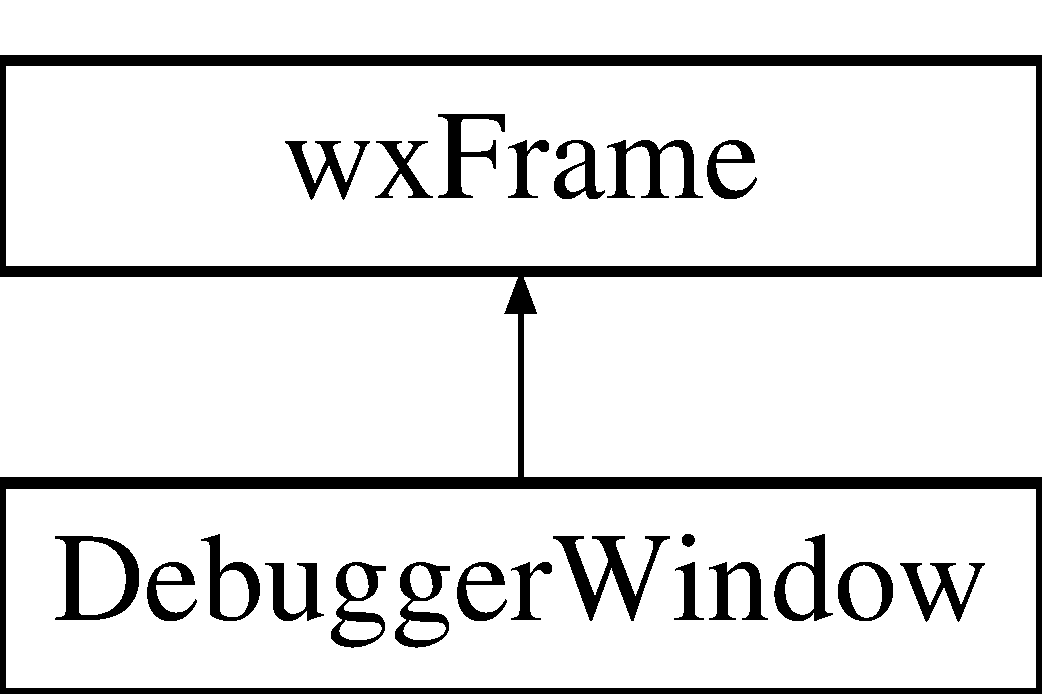
\includegraphics[height=2.000000cm]{class_debugger_window}
\end{center}
\end{figure}
\subsection*{Public Member Functions}
\begin{DoxyCompactItemize}
\item 
\hyperlink{class_debugger_window_ae72a6bed32d587f5dc4d301242ae5720}{Debugger\+Window} (wx\+Window $\ast$parent, const wx\+String \&title, const wx\+Point \&pos, const wx\+Size \&size)
\item 
\hyperlink{class_debugger_window_a59bb9cc5a75d6d953d940c112c5a38a3}{$\sim$\+Debugger\+Window} ()
\item 
void \hyperlink{class_debugger_window_a58b244eaf8947c48629eca294a4aa37b}{view} (uint32\+\_\+t start\+\_\+addr, uint32\+\_\+t end\+\_\+addr)
\item 
void \hyperlink{class_debugger_window_a00a164c597b3faa9c69360e60cb55cf6}{On\+C\+P\+U\+Step} (wx\+Command\+Event \&event)
\item 
\hyperlink{class_debugger_window_a4ec20c97fe9716957caf2d4c19cdaff4}{wx\+D\+E\+C\+L\+A\+R\+E\+\_\+\+E\+V\+E\+N\+T\+\_\+\+T\+A\+B\+LE} ()
\end{DoxyCompactItemize}
\subsection*{Public Attributes}
\begin{DoxyCompactItemize}
\item 
wx\+List\+Box $\ast$ \hyperlink{class_debugger_window_a5907a83225613994ce1bf78e170f3e69}{memory\+\_\+listbox} = N\+U\+LL
\item 
wx\+Button $\ast$ \hyperlink{class_debugger_window_a8cbfc7ff4b60b4ce45f94af2771e222a}{cpu\+\_\+step} = N\+U\+LL
\end{DoxyCompactItemize}


\subsection{Constructor \& Destructor Documentation}
\mbox{\Hypertarget{class_debugger_window_ae72a6bed32d587f5dc4d301242ae5720}\label{class_debugger_window_ae72a6bed32d587f5dc4d301242ae5720}} 
\index{Debugger\+Window@{Debugger\+Window}!Debugger\+Window@{Debugger\+Window}}
\index{Debugger\+Window@{Debugger\+Window}!Debugger\+Window@{Debugger\+Window}}
\subsubsection{\texorpdfstring{Debugger\+Window()}{DebuggerWindow()}}
{\footnotesize\ttfamily Debugger\+Window\+::\+Debugger\+Window (\begin{DoxyParamCaption}\item[{wx\+Window $\ast$}]{parent,  }\item[{const wx\+String \&}]{title,  }\item[{const wx\+Point \&}]{pos,  }\item[{const wx\+Size \&}]{size }\end{DoxyParamCaption})}

\mbox{\Hypertarget{class_debugger_window_a59bb9cc5a75d6d953d940c112c5a38a3}\label{class_debugger_window_a59bb9cc5a75d6d953d940c112c5a38a3}} 
\index{Debugger\+Window@{Debugger\+Window}!````~Debugger\+Window@{$\sim$\+Debugger\+Window}}
\index{````~Debugger\+Window@{$\sim$\+Debugger\+Window}!Debugger\+Window@{Debugger\+Window}}
\subsubsection{\texorpdfstring{$\sim$\+Debugger\+Window()}{~DebuggerWindow()}}
{\footnotesize\ttfamily Debugger\+Window\+::$\sim$\+Debugger\+Window (\begin{DoxyParamCaption}{ }\end{DoxyParamCaption})}



\subsection{Member Function Documentation}
\mbox{\Hypertarget{class_debugger_window_a00a164c597b3faa9c69360e60cb55cf6}\label{class_debugger_window_a00a164c597b3faa9c69360e60cb55cf6}} 
\index{Debugger\+Window@{Debugger\+Window}!On\+C\+P\+U\+Step@{On\+C\+P\+U\+Step}}
\index{On\+C\+P\+U\+Step@{On\+C\+P\+U\+Step}!Debugger\+Window@{Debugger\+Window}}
\subsubsection{\texorpdfstring{On\+C\+P\+U\+Step()}{OnCPUStep()}}
{\footnotesize\ttfamily void Debugger\+Window\+::\+On\+C\+P\+U\+Step (\begin{DoxyParamCaption}\item[{wx\+Command\+Event \&}]{event }\end{DoxyParamCaption})}

\mbox{\Hypertarget{class_debugger_window_a58b244eaf8947c48629eca294a4aa37b}\label{class_debugger_window_a58b244eaf8947c48629eca294a4aa37b}} 
\index{Debugger\+Window@{Debugger\+Window}!view@{view}}
\index{view@{view}!Debugger\+Window@{Debugger\+Window}}
\subsubsection{\texorpdfstring{view()}{view()}}
{\footnotesize\ttfamily void Debugger\+Window\+::view (\begin{DoxyParamCaption}\item[{uint32\+\_\+t}]{start\+\_\+addr,  }\item[{uint32\+\_\+t}]{end\+\_\+addr }\end{DoxyParamCaption})}

\mbox{\Hypertarget{class_debugger_window_a4ec20c97fe9716957caf2d4c19cdaff4}\label{class_debugger_window_a4ec20c97fe9716957caf2d4c19cdaff4}} 
\index{Debugger\+Window@{Debugger\+Window}!wx\+D\+E\+C\+L\+A\+R\+E\+\_\+\+E\+V\+E\+N\+T\+\_\+\+T\+A\+B\+LE@{wx\+D\+E\+C\+L\+A\+R\+E\+\_\+\+E\+V\+E\+N\+T\+\_\+\+T\+A\+B\+LE}}
\index{wx\+D\+E\+C\+L\+A\+R\+E\+\_\+\+E\+V\+E\+N\+T\+\_\+\+T\+A\+B\+LE@{wx\+D\+E\+C\+L\+A\+R\+E\+\_\+\+E\+V\+E\+N\+T\+\_\+\+T\+A\+B\+LE}!Debugger\+Window@{Debugger\+Window}}
\subsubsection{\texorpdfstring{wx\+D\+E\+C\+L\+A\+R\+E\+\_\+\+E\+V\+E\+N\+T\+\_\+\+T\+A\+B\+L\+E()}{wxDECLARE\_EVENT\_TABLE()}}
{\footnotesize\ttfamily Debugger\+Window\+::wx\+D\+E\+C\+L\+A\+R\+E\+\_\+\+E\+V\+E\+N\+T\+\_\+\+T\+A\+B\+LE (\begin{DoxyParamCaption}{ }\end{DoxyParamCaption})}



\subsection{Member Data Documentation}
\mbox{\Hypertarget{class_debugger_window_a8cbfc7ff4b60b4ce45f94af2771e222a}\label{class_debugger_window_a8cbfc7ff4b60b4ce45f94af2771e222a}} 
\index{Debugger\+Window@{Debugger\+Window}!cpu\+\_\+step@{cpu\+\_\+step}}
\index{cpu\+\_\+step@{cpu\+\_\+step}!Debugger\+Window@{Debugger\+Window}}
\subsubsection{\texorpdfstring{cpu\+\_\+step}{cpu\_step}}
{\footnotesize\ttfamily wx\+Button$\ast$ Debugger\+Window\+::cpu\+\_\+step = N\+U\+LL}

\mbox{\Hypertarget{class_debugger_window_a5907a83225613994ce1bf78e170f3e69}\label{class_debugger_window_a5907a83225613994ce1bf78e170f3e69}} 
\index{Debugger\+Window@{Debugger\+Window}!memory\+\_\+listbox@{memory\+\_\+listbox}}
\index{memory\+\_\+listbox@{memory\+\_\+listbox}!Debugger\+Window@{Debugger\+Window}}
\subsubsection{\texorpdfstring{memory\+\_\+listbox}{memory\_listbox}}
{\footnotesize\ttfamily wx\+List\+Box$\ast$ Debugger\+Window\+::memory\+\_\+listbox = N\+U\+LL}



The documentation for this class was generated from the following files\+:\begin{DoxyCompactItemize}
\item 
include/\hyperlink{ultra64_8h}{ultra64.\+h}\item 
src/\hyperlink{ultra64_8cpp}{ultra64.\+cpp}\end{DoxyCompactItemize}

\hypertarget{class_main_window}{}\section{Main\+Window Class Reference}
\label{class_main_window}\index{Main\+Window@{Main\+Window}}


{\ttfamily \#include $<$ultra64.\+h$>$}

Inheritance diagram for Main\+Window\+:\begin{figure}[H]
\begin{center}
\leavevmode
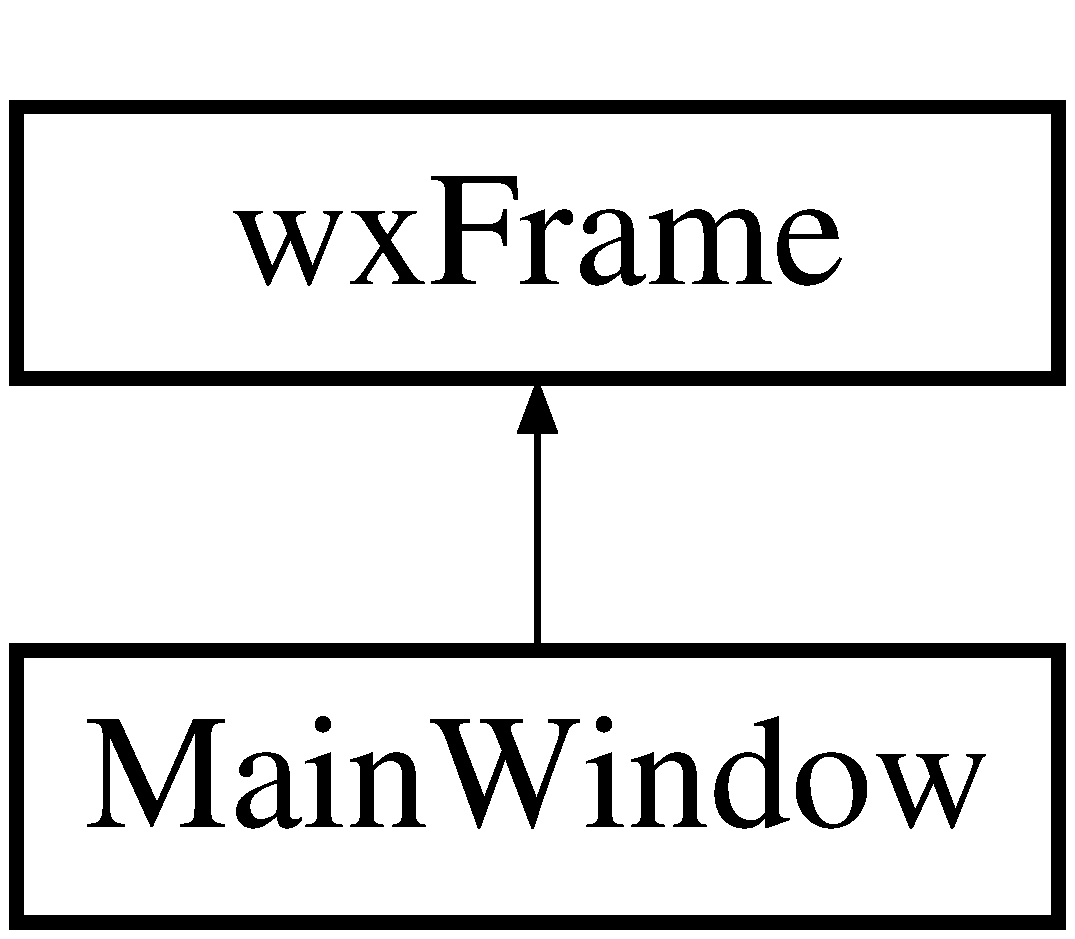
\includegraphics[height=2.000000cm]{class_main_window}
\end{center}
\end{figure}
\subsection*{Public Member Functions}
\begin{DoxyCompactItemize}
\item 
\hyperlink{class_main_window_ab5bd7c178471f31f5c7f20fad6446382}{Main\+Window} (const wx\+String \&title, const wx\+Point \&pos, const wx\+Size \&size)
\end{DoxyCompactItemize}
\subsection*{Private Member Functions}
\begin{DoxyCompactItemize}
\item 
void \hyperlink{class_main_window_a28e8accc0a0157573cd8f9aad24c0c70}{On\+Open\+R\+OM} (wx\+Command\+Event \&event)
\item 
void \hyperlink{class_main_window_a593f2d52215a2cf7d8cf79ae1e792df9}{On\+Open\+P\+I\+F\+R\+OM} (wx\+Command\+Event \&event)
\item 
void \hyperlink{class_main_window_a1a605e490ac5deeb89ed16cfc871bf3f}{On\+Exit} (wx\+Command\+Event \&event)
\item 
void \hyperlink{class_main_window_afa16bbfe7c1f9f4ba9192210ca68d996}{On\+About} (wx\+Command\+Event \&event)
\item 
void \hyperlink{class_main_window_ad417cf49adddf2caaab6b42eaca297e3}{On\+Debug\+P\+I\+F\+R\+OM} (wx\+Command\+Event \&event)
\item 
void \hyperlink{class_main_window_af112afb589538613e918372017a64084}{On\+Debug\+R\+OM} (wx\+Command\+Event \&event)
\item 
void \hyperlink{class_main_window_a19dd4cc763eefb616417f390a5ecd1fa}{On\+Debug\+Registers} (wx\+Command\+Event \&event)
\item 
\hyperlink{class_main_window_ae2ff5d7859e51963c5c07ab11583021a}{wx\+D\+E\+C\+L\+A\+R\+E\+\_\+\+E\+V\+E\+N\+T\+\_\+\+T\+A\+B\+LE} ()
\end{DoxyCompactItemize}


\subsection{Constructor \& Destructor Documentation}
\mbox{\Hypertarget{class_main_window_ab5bd7c178471f31f5c7f20fad6446382}\label{class_main_window_ab5bd7c178471f31f5c7f20fad6446382}} 
\index{Main\+Window@{Main\+Window}!Main\+Window@{Main\+Window}}
\index{Main\+Window@{Main\+Window}!Main\+Window@{Main\+Window}}
\subsubsection{\texorpdfstring{Main\+Window()}{MainWindow()}}
{\footnotesize\ttfamily Main\+Window\+::\+Main\+Window (\begin{DoxyParamCaption}\item[{const wx\+String \&}]{title,  }\item[{const wx\+Point \&}]{pos,  }\item[{const wx\+Size \&}]{size }\end{DoxyParamCaption})}



\subsection{Member Function Documentation}
\mbox{\Hypertarget{class_main_window_afa16bbfe7c1f9f4ba9192210ca68d996}\label{class_main_window_afa16bbfe7c1f9f4ba9192210ca68d996}} 
\index{Main\+Window@{Main\+Window}!On\+About@{On\+About}}
\index{On\+About@{On\+About}!Main\+Window@{Main\+Window}}
\subsubsection{\texorpdfstring{On\+About()}{OnAbout()}}
{\footnotesize\ttfamily void Main\+Window\+::\+On\+About (\begin{DoxyParamCaption}\item[{wx\+Command\+Event \&}]{event }\end{DoxyParamCaption})\hspace{0.3cm}{\ttfamily [private]}}

\mbox{\Hypertarget{class_main_window_ad417cf49adddf2caaab6b42eaca297e3}\label{class_main_window_ad417cf49adddf2caaab6b42eaca297e3}} 
\index{Main\+Window@{Main\+Window}!On\+Debug\+P\+I\+F\+R\+OM@{On\+Debug\+P\+I\+F\+R\+OM}}
\index{On\+Debug\+P\+I\+F\+R\+OM@{On\+Debug\+P\+I\+F\+R\+OM}!Main\+Window@{Main\+Window}}
\subsubsection{\texorpdfstring{On\+Debug\+P\+I\+F\+R\+O\+M()}{OnDebugPIFROM()}}
{\footnotesize\ttfamily void Main\+Window\+::\+On\+Debug\+P\+I\+F\+R\+OM (\begin{DoxyParamCaption}\item[{wx\+Command\+Event \&}]{event }\end{DoxyParamCaption})\hspace{0.3cm}{\ttfamily [private]}}

\mbox{\Hypertarget{class_main_window_a19dd4cc763eefb616417f390a5ecd1fa}\label{class_main_window_a19dd4cc763eefb616417f390a5ecd1fa}} 
\index{Main\+Window@{Main\+Window}!On\+Debug\+Registers@{On\+Debug\+Registers}}
\index{On\+Debug\+Registers@{On\+Debug\+Registers}!Main\+Window@{Main\+Window}}
\subsubsection{\texorpdfstring{On\+Debug\+Registers()}{OnDebugRegisters()}}
{\footnotesize\ttfamily void Main\+Window\+::\+On\+Debug\+Registers (\begin{DoxyParamCaption}\item[{wx\+Command\+Event \&}]{event }\end{DoxyParamCaption})\hspace{0.3cm}{\ttfamily [private]}}

\mbox{\Hypertarget{class_main_window_af112afb589538613e918372017a64084}\label{class_main_window_af112afb589538613e918372017a64084}} 
\index{Main\+Window@{Main\+Window}!On\+Debug\+R\+OM@{On\+Debug\+R\+OM}}
\index{On\+Debug\+R\+OM@{On\+Debug\+R\+OM}!Main\+Window@{Main\+Window}}
\subsubsection{\texorpdfstring{On\+Debug\+R\+O\+M()}{OnDebugROM()}}
{\footnotesize\ttfamily void Main\+Window\+::\+On\+Debug\+R\+OM (\begin{DoxyParamCaption}\item[{wx\+Command\+Event \&}]{event }\end{DoxyParamCaption})\hspace{0.3cm}{\ttfamily [private]}}

\mbox{\Hypertarget{class_main_window_a1a605e490ac5deeb89ed16cfc871bf3f}\label{class_main_window_a1a605e490ac5deeb89ed16cfc871bf3f}} 
\index{Main\+Window@{Main\+Window}!On\+Exit@{On\+Exit}}
\index{On\+Exit@{On\+Exit}!Main\+Window@{Main\+Window}}
\subsubsection{\texorpdfstring{On\+Exit()}{OnExit()}}
{\footnotesize\ttfamily void Main\+Window\+::\+On\+Exit (\begin{DoxyParamCaption}\item[{wx\+Command\+Event \&}]{event }\end{DoxyParamCaption})\hspace{0.3cm}{\ttfamily [private]}}

\mbox{\Hypertarget{class_main_window_a593f2d52215a2cf7d8cf79ae1e792df9}\label{class_main_window_a593f2d52215a2cf7d8cf79ae1e792df9}} 
\index{Main\+Window@{Main\+Window}!On\+Open\+P\+I\+F\+R\+OM@{On\+Open\+P\+I\+F\+R\+OM}}
\index{On\+Open\+P\+I\+F\+R\+OM@{On\+Open\+P\+I\+F\+R\+OM}!Main\+Window@{Main\+Window}}
\subsubsection{\texorpdfstring{On\+Open\+P\+I\+F\+R\+O\+M()}{OnOpenPIFROM()}}
{\footnotesize\ttfamily void Main\+Window\+::\+On\+Open\+P\+I\+F\+R\+OM (\begin{DoxyParamCaption}\item[{wx\+Command\+Event \&}]{event }\end{DoxyParamCaption})\hspace{0.3cm}{\ttfamily [private]}}

\mbox{\Hypertarget{class_main_window_a28e8accc0a0157573cd8f9aad24c0c70}\label{class_main_window_a28e8accc0a0157573cd8f9aad24c0c70}} 
\index{Main\+Window@{Main\+Window}!On\+Open\+R\+OM@{On\+Open\+R\+OM}}
\index{On\+Open\+R\+OM@{On\+Open\+R\+OM}!Main\+Window@{Main\+Window}}
\subsubsection{\texorpdfstring{On\+Open\+R\+O\+M()}{OnOpenROM()}}
{\footnotesize\ttfamily void Main\+Window\+::\+On\+Open\+R\+OM (\begin{DoxyParamCaption}\item[{wx\+Command\+Event \&}]{event }\end{DoxyParamCaption})\hspace{0.3cm}{\ttfamily [private]}}

\mbox{\Hypertarget{class_main_window_ae2ff5d7859e51963c5c07ab11583021a}\label{class_main_window_ae2ff5d7859e51963c5c07ab11583021a}} 
\index{Main\+Window@{Main\+Window}!wx\+D\+E\+C\+L\+A\+R\+E\+\_\+\+E\+V\+E\+N\+T\+\_\+\+T\+A\+B\+LE@{wx\+D\+E\+C\+L\+A\+R\+E\+\_\+\+E\+V\+E\+N\+T\+\_\+\+T\+A\+B\+LE}}
\index{wx\+D\+E\+C\+L\+A\+R\+E\+\_\+\+E\+V\+E\+N\+T\+\_\+\+T\+A\+B\+LE@{wx\+D\+E\+C\+L\+A\+R\+E\+\_\+\+E\+V\+E\+N\+T\+\_\+\+T\+A\+B\+LE}!Main\+Window@{Main\+Window}}
\subsubsection{\texorpdfstring{wx\+D\+E\+C\+L\+A\+R\+E\+\_\+\+E\+V\+E\+N\+T\+\_\+\+T\+A\+B\+L\+E()}{wxDECLARE\_EVENT\_TABLE()}}
{\footnotesize\ttfamily Main\+Window\+::wx\+D\+E\+C\+L\+A\+R\+E\+\_\+\+E\+V\+E\+N\+T\+\_\+\+T\+A\+B\+LE (\begin{DoxyParamCaption}{ }\end{DoxyParamCaption})\hspace{0.3cm}{\ttfamily [private]}}



The documentation for this class was generated from the following files\+:\begin{DoxyCompactItemize}
\item 
include/\hyperlink{ultra64_8h}{ultra64.\+h}\item 
src/\hyperlink{ultra64_8cpp}{ultra64.\+cpp}\end{DoxyCompactItemize}

\hypertarget{structultra64_1_1memory__section}{}\section{ultra64\+:\+:memory\+\_\+section Struct Reference}
\label{structultra64_1_1memory__section}\index{ultra64\+::memory\+\_\+section@{ultra64\+::memory\+\_\+section}}


{\ttfamily \#include $<$memory.\+h$>$}

\subsection*{Public Attributes}
\begin{DoxyCompactItemize}
\item 
uint32\+\_\+t \hyperlink{structultra64_1_1memory__section_a0b3b346659febefd75c3b57ad4362179}{offset} = 0
\item 
void $\ast$ \hyperlink{structultra64_1_1memory__section_affbc3bd34afd0a4d69a31182d5a9e231}{ptr} = nullptr
\end{DoxyCompactItemize}


\subsection{Member Data Documentation}
\mbox{\Hypertarget{structultra64_1_1memory__section_a0b3b346659febefd75c3b57ad4362179}\label{structultra64_1_1memory__section_a0b3b346659febefd75c3b57ad4362179}} 
\index{ultra64\+::memory\+\_\+section@{ultra64\+::memory\+\_\+section}!offset@{offset}}
\index{offset@{offset}!ultra64\+::memory\+\_\+section@{ultra64\+::memory\+\_\+section}}
\subsubsection{\texorpdfstring{offset}{offset}}
{\footnotesize\ttfamily uint32\+\_\+t ultra64\+::memory\+\_\+section\+::offset = 0}

\mbox{\Hypertarget{structultra64_1_1memory__section_affbc3bd34afd0a4d69a31182d5a9e231}\label{structultra64_1_1memory__section_affbc3bd34afd0a4d69a31182d5a9e231}} 
\index{ultra64\+::memory\+\_\+section@{ultra64\+::memory\+\_\+section}!ptr@{ptr}}
\index{ptr@{ptr}!ultra64\+::memory\+\_\+section@{ultra64\+::memory\+\_\+section}}
\subsubsection{\texorpdfstring{ptr}{ptr}}
{\footnotesize\ttfamily void$\ast$ ultra64\+::memory\+\_\+section\+::ptr = nullptr}



The documentation for this struct was generated from the following file\+:\begin{DoxyCompactItemize}
\item 
include/\hyperlink{memory_8h}{memory.\+h}\end{DoxyCompactItemize}

\hypertarget{classultra64_1_1_m_m_u}{}\section{ultra64\+:\+:M\+MU Class Reference}
\label{classultra64_1_1_m_m_u}\index{ultra64\+::\+M\+MU@{ultra64\+::\+M\+MU}}


{\ttfamily \#include $<$memory.\+h$>$}

\subsection*{Public Member Functions}
\begin{DoxyCompactItemize}
\item 
\hyperlink{classultra64_1_1_m_m_u_a2fdb1cba73825c3988f2a1216e806c7c}{M\+MU} ()
\item 
\hyperlink{classultra64_1_1_m_m_u_a9ee9394ce2502116d7773d5f6123a24e}{$\sim$\+M\+MU} ()
\item 
void \hyperlink{classultra64_1_1_m_m_u_aba8d57fd9862ade57d54b1581dd93682}{attach\+\_\+rom} (unsigned char $\ast$\hyperlink{classultra64_1_1_m_m_u_a7ad1ee24b85de6513bf53ba6c963f529}{rom}, size\+\_\+t sz)
\item 
uint8\+\_\+t \hyperlink{classultra64_1_1_m_m_u_a8cdfede1aebd137ae20dfda84f0e23a1}{read\+\_\+byte} (uint32\+\_\+t addr)
\item 
uint16\+\_\+t \hyperlink{classultra64_1_1_m_m_u_a0e4bb683637877aba6c5def53c719b0f}{read\+\_\+hword} (uint32\+\_\+t addr)
\item 
uint32\+\_\+t \hyperlink{classultra64_1_1_m_m_u_a894a894a4340798c457e7ad41c3dd2ff}{read\+\_\+word} (uint32\+\_\+t addr)
\item 
void \hyperlink{classultra64_1_1_m_m_u_aac98a1626ea3f4168c0a3c5ae6036289}{write\+\_\+byte} (uint32\+\_\+t addr, uint8\+\_\+t value)
\item 
void \hyperlink{classultra64_1_1_m_m_u_ab594e1f0fe4958b521af5408aab46456}{write\+\_\+hword} (uint32\+\_\+t addr, uint16\+\_\+t value)
\item 
void \hyperlink{classultra64_1_1_m_m_u_a4dd4d9827368407081996591918fee9c}{write\+\_\+word} (uint32\+\_\+t addr, uint32\+\_\+t value)
\end{DoxyCompactItemize}
\subsection*{Private Member Functions}
\begin{DoxyCompactItemize}
\item 
\hyperlink{structultra64_1_1memory__section}{memory\+\_\+section} \hyperlink{classultra64_1_1_m_m_u_a30dc6643202a4b3a435cd7458fb4b6b4}{get\+\_\+section} (uint32\+\_\+t addr)
\end{DoxyCompactItemize}
\subsection*{Private Attributes}
\begin{DoxyCompactItemize}
\item 
unsigned char $\ast$ \hyperlink{classultra64_1_1_m_m_u_a3c06ec9b1a0385a54e46aa1b6763d190}{pif\+\_\+rom} = new unsigned char\mbox{[}0x7\+B\+F\mbox{]}
\item 
unsigned char $\ast$ \hyperlink{classultra64_1_1_m_m_u_a9d041024d1764dde4738d401882e2c75}{pif\+\_\+ram} = new unsigned char\mbox{[}0x40\mbox{]}
\item 
unsigned char $\ast$ \hyperlink{classultra64_1_1_m_m_u_a7ad1ee24b85de6513bf53ba6c963f529}{rom} = nullptr
\item 
size\+\_\+t \hyperlink{classultra64_1_1_m_m_u_afb879907a642040c391b4fce51840564}{rom\+\_\+sz} = 0
\item 
unsigned char $\ast$ \hyperlink{classultra64_1_1_m_m_u_af1ecbc3316b0d24d31ef0c06264cc452}{rdram} = new unsigned char\mbox{[}0x400000\mbox{]}
\item 
unsigned char $\ast$ \hyperlink{classultra64_1_1_m_m_u_ae002e380f5261812fa2a6b37ab6dd9fa}{rdram\+\_\+registers} = new unsigned char\mbox{[}0x28\mbox{]}
\item 
unsigned char $\ast$ \hyperlink{classultra64_1_1_m_m_u_a860851cd6f4767cd238526e6fcadb0dc}{sp\+\_\+dmem} = new unsigned char\mbox{[}0x1000\mbox{]}
\item 
unsigned char $\ast$ \hyperlink{classultra64_1_1_m_m_u_abf6db7a046cc2b6146d3e52327d69bdb}{sp\+\_\+imem} = new unsigned char\mbox{[}0x1000\mbox{]}
\item 
unsigned char $\ast$ \hyperlink{classultra64_1_1_m_m_u_a9ca940d08ce7429fe1cd2440bc508800}{sp\+\_\+registers} = new unsigned char\mbox{[}0x20\mbox{]}
\item 
unsigned char $\ast$ \hyperlink{classultra64_1_1_m_m_u_aad78b94bfb2096b563b7de68cddca76c}{sp\+\_\+registers2} = new unsigned char\mbox{[}0x8\mbox{]}
\item 
unsigned char $\ast$ \hyperlink{classultra64_1_1_m_m_u_a3054f197e8e6b801272dc87d8678aed8}{pi\+\_\+registers} = new unsigned char\mbox{[}0x34\mbox{]}
\item 
unsigned char $\ast$ \hyperlink{classultra64_1_1_m_m_u_ab72c6d87f83e2c99ed0e2e9f43f1f240}{vi\+\_\+registers} = new unsigned char\mbox{[}0x38\mbox{]}
\item 
unsigned char $\ast$ \hyperlink{classultra64_1_1_m_m_u_a30a9501b79dbeffb191b7f89c375e9e0}{ai\+\_\+registers} = new unsigned char\mbox{[}0x18\mbox{]}
\item 
unsigned char $\ast$ \hyperlink{classultra64_1_1_m_m_u_a9d4a71c847de246e9a23149921e7312e}{dp\+\_\+command\+\_\+registers} = new unsigned char\mbox{[}0x20\mbox{]}
\item 
unsigned char $\ast$ \hyperlink{classultra64_1_1_m_m_u_af6b87f01506b320306aefde9d1d7de8c}{dp\+\_\+span\+\_\+registers} = new unsigned char\mbox{[}0x10\mbox{]}
\item 
unsigned char $\ast$ \hyperlink{classultra64_1_1_m_m_u_a470447b5a22c8081ee5cd1da7f3c4724}{mi\+\_\+registers} = new unsigned char\mbox{[}0x10\mbox{]}
\item 
unsigned char $\ast$ \hyperlink{classultra64_1_1_m_m_u_a73128f9d67e5ebb8182c4f57d2b5af3f}{ri\+\_\+registers} = new unsigned char\mbox{[}0x20\mbox{]}
\item 
unsigned char $\ast$ \hyperlink{classultra64_1_1_m_m_u_a0256b081d410cd7375f4837326326dd9}{si\+\_\+registers} = new unsigned char\mbox{[}0x1\+C\mbox{]}
\end{DoxyCompactItemize}


\subsection{Constructor \& Destructor Documentation}
\mbox{\Hypertarget{classultra64_1_1_m_m_u_a2fdb1cba73825c3988f2a1216e806c7c}\label{classultra64_1_1_m_m_u_a2fdb1cba73825c3988f2a1216e806c7c}} 
\index{ultra64\+::\+M\+MU@{ultra64\+::\+M\+MU}!M\+MU@{M\+MU}}
\index{M\+MU@{M\+MU}!ultra64\+::\+M\+MU@{ultra64\+::\+M\+MU}}
\subsubsection{\texorpdfstring{M\+M\+U()}{MMU()}}
{\footnotesize\ttfamily ultra64\+::\+M\+M\+U\+::\+M\+MU (\begin{DoxyParamCaption}{ }\end{DoxyParamCaption})}

\mbox{\Hypertarget{classultra64_1_1_m_m_u_a9ee9394ce2502116d7773d5f6123a24e}\label{classultra64_1_1_m_m_u_a9ee9394ce2502116d7773d5f6123a24e}} 
\index{ultra64\+::\+M\+MU@{ultra64\+::\+M\+MU}!````~M\+MU@{$\sim$\+M\+MU}}
\index{````~M\+MU@{$\sim$\+M\+MU}!ultra64\+::\+M\+MU@{ultra64\+::\+M\+MU}}
\subsubsection{\texorpdfstring{$\sim$\+M\+M\+U()}{~MMU()}}
{\footnotesize\ttfamily ultra64\+::\+M\+M\+U\+::$\sim$\+M\+MU (\begin{DoxyParamCaption}{ }\end{DoxyParamCaption})}



\subsection{Member Function Documentation}
\mbox{\Hypertarget{classultra64_1_1_m_m_u_aba8d57fd9862ade57d54b1581dd93682}\label{classultra64_1_1_m_m_u_aba8d57fd9862ade57d54b1581dd93682}} 
\index{ultra64\+::\+M\+MU@{ultra64\+::\+M\+MU}!attach\+\_\+rom@{attach\+\_\+rom}}
\index{attach\+\_\+rom@{attach\+\_\+rom}!ultra64\+::\+M\+MU@{ultra64\+::\+M\+MU}}
\subsubsection{\texorpdfstring{attach\+\_\+rom()}{attach\_rom()}}
{\footnotesize\ttfamily void ultra64\+::\+M\+M\+U\+::attach\+\_\+rom (\begin{DoxyParamCaption}\item[{unsigned char $\ast$}]{rom,  }\item[{size\+\_\+t}]{sz }\end{DoxyParamCaption})}

\mbox{\Hypertarget{classultra64_1_1_m_m_u_a30dc6643202a4b3a435cd7458fb4b6b4}\label{classultra64_1_1_m_m_u_a30dc6643202a4b3a435cd7458fb4b6b4}} 
\index{ultra64\+::\+M\+MU@{ultra64\+::\+M\+MU}!get\+\_\+section@{get\+\_\+section}}
\index{get\+\_\+section@{get\+\_\+section}!ultra64\+::\+M\+MU@{ultra64\+::\+M\+MU}}
\subsubsection{\texorpdfstring{get\+\_\+section()}{get\_section()}}
{\footnotesize\ttfamily \hyperlink{structultra64_1_1memory__section}{memory\+\_\+section} ultra64\+::\+M\+M\+U\+::get\+\_\+section (\begin{DoxyParamCaption}\item[{uint32\+\_\+t}]{addr }\end{DoxyParamCaption})\hspace{0.3cm}{\ttfamily [private]}}

\mbox{\Hypertarget{classultra64_1_1_m_m_u_a8cdfede1aebd137ae20dfda84f0e23a1}\label{classultra64_1_1_m_m_u_a8cdfede1aebd137ae20dfda84f0e23a1}} 
\index{ultra64\+::\+M\+MU@{ultra64\+::\+M\+MU}!read\+\_\+byte@{read\+\_\+byte}}
\index{read\+\_\+byte@{read\+\_\+byte}!ultra64\+::\+M\+MU@{ultra64\+::\+M\+MU}}
\subsubsection{\texorpdfstring{read\+\_\+byte()}{read\_byte()}}
{\footnotesize\ttfamily uint8\+\_\+t ultra64\+::\+M\+M\+U\+::read\+\_\+byte (\begin{DoxyParamCaption}\item[{uint32\+\_\+t}]{addr }\end{DoxyParamCaption})}

\mbox{\Hypertarget{classultra64_1_1_m_m_u_a0e4bb683637877aba6c5def53c719b0f}\label{classultra64_1_1_m_m_u_a0e4bb683637877aba6c5def53c719b0f}} 
\index{ultra64\+::\+M\+MU@{ultra64\+::\+M\+MU}!read\+\_\+hword@{read\+\_\+hword}}
\index{read\+\_\+hword@{read\+\_\+hword}!ultra64\+::\+M\+MU@{ultra64\+::\+M\+MU}}
\subsubsection{\texorpdfstring{read\+\_\+hword()}{read\_hword()}}
{\footnotesize\ttfamily uint16\+\_\+t ultra64\+::\+M\+M\+U\+::read\+\_\+hword (\begin{DoxyParamCaption}\item[{uint32\+\_\+t}]{addr }\end{DoxyParamCaption})}

\mbox{\Hypertarget{classultra64_1_1_m_m_u_a894a894a4340798c457e7ad41c3dd2ff}\label{classultra64_1_1_m_m_u_a894a894a4340798c457e7ad41c3dd2ff}} 
\index{ultra64\+::\+M\+MU@{ultra64\+::\+M\+MU}!read\+\_\+word@{read\+\_\+word}}
\index{read\+\_\+word@{read\+\_\+word}!ultra64\+::\+M\+MU@{ultra64\+::\+M\+MU}}
\subsubsection{\texorpdfstring{read\+\_\+word()}{read\_word()}}
{\footnotesize\ttfamily uint32\+\_\+t ultra64\+::\+M\+M\+U\+::read\+\_\+word (\begin{DoxyParamCaption}\item[{uint32\+\_\+t}]{addr }\end{DoxyParamCaption})}

\mbox{\Hypertarget{classultra64_1_1_m_m_u_aac98a1626ea3f4168c0a3c5ae6036289}\label{classultra64_1_1_m_m_u_aac98a1626ea3f4168c0a3c5ae6036289}} 
\index{ultra64\+::\+M\+MU@{ultra64\+::\+M\+MU}!write\+\_\+byte@{write\+\_\+byte}}
\index{write\+\_\+byte@{write\+\_\+byte}!ultra64\+::\+M\+MU@{ultra64\+::\+M\+MU}}
\subsubsection{\texorpdfstring{write\+\_\+byte()}{write\_byte()}}
{\footnotesize\ttfamily void ultra64\+::\+M\+M\+U\+::write\+\_\+byte (\begin{DoxyParamCaption}\item[{uint32\+\_\+t}]{addr,  }\item[{uint8\+\_\+t}]{value }\end{DoxyParamCaption})}

\mbox{\Hypertarget{classultra64_1_1_m_m_u_ab594e1f0fe4958b521af5408aab46456}\label{classultra64_1_1_m_m_u_ab594e1f0fe4958b521af5408aab46456}} 
\index{ultra64\+::\+M\+MU@{ultra64\+::\+M\+MU}!write\+\_\+hword@{write\+\_\+hword}}
\index{write\+\_\+hword@{write\+\_\+hword}!ultra64\+::\+M\+MU@{ultra64\+::\+M\+MU}}
\subsubsection{\texorpdfstring{write\+\_\+hword()}{write\_hword()}}
{\footnotesize\ttfamily void ultra64\+::\+M\+M\+U\+::write\+\_\+hword (\begin{DoxyParamCaption}\item[{uint32\+\_\+t}]{addr,  }\item[{uint16\+\_\+t}]{value }\end{DoxyParamCaption})}

\mbox{\Hypertarget{classultra64_1_1_m_m_u_a4dd4d9827368407081996591918fee9c}\label{classultra64_1_1_m_m_u_a4dd4d9827368407081996591918fee9c}} 
\index{ultra64\+::\+M\+MU@{ultra64\+::\+M\+MU}!write\+\_\+word@{write\+\_\+word}}
\index{write\+\_\+word@{write\+\_\+word}!ultra64\+::\+M\+MU@{ultra64\+::\+M\+MU}}
\subsubsection{\texorpdfstring{write\+\_\+word()}{write\_word()}}
{\footnotesize\ttfamily void ultra64\+::\+M\+M\+U\+::write\+\_\+word (\begin{DoxyParamCaption}\item[{uint32\+\_\+t}]{addr,  }\item[{uint32\+\_\+t}]{value }\end{DoxyParamCaption})}



\subsection{Member Data Documentation}
\mbox{\Hypertarget{classultra64_1_1_m_m_u_a30a9501b79dbeffb191b7f89c375e9e0}\label{classultra64_1_1_m_m_u_a30a9501b79dbeffb191b7f89c375e9e0}} 
\index{ultra64\+::\+M\+MU@{ultra64\+::\+M\+MU}!ai\+\_\+registers@{ai\+\_\+registers}}
\index{ai\+\_\+registers@{ai\+\_\+registers}!ultra64\+::\+M\+MU@{ultra64\+::\+M\+MU}}
\subsubsection{\texorpdfstring{ai\+\_\+registers}{ai\_registers}}
{\footnotesize\ttfamily unsigned char$\ast$ ultra64\+::\+M\+M\+U\+::ai\+\_\+registers = new unsigned char\mbox{[}0x18\mbox{]}\hspace{0.3cm}{\ttfamily [private]}}

\mbox{\Hypertarget{classultra64_1_1_m_m_u_a9d4a71c847de246e9a23149921e7312e}\label{classultra64_1_1_m_m_u_a9d4a71c847de246e9a23149921e7312e}} 
\index{ultra64\+::\+M\+MU@{ultra64\+::\+M\+MU}!dp\+\_\+command\+\_\+registers@{dp\+\_\+command\+\_\+registers}}
\index{dp\+\_\+command\+\_\+registers@{dp\+\_\+command\+\_\+registers}!ultra64\+::\+M\+MU@{ultra64\+::\+M\+MU}}
\subsubsection{\texorpdfstring{dp\+\_\+command\+\_\+registers}{dp\_command\_registers}}
{\footnotesize\ttfamily unsigned char$\ast$ ultra64\+::\+M\+M\+U\+::dp\+\_\+command\+\_\+registers = new unsigned char\mbox{[}0x20\mbox{]}\hspace{0.3cm}{\ttfamily [private]}}

\mbox{\Hypertarget{classultra64_1_1_m_m_u_af6b87f01506b320306aefde9d1d7de8c}\label{classultra64_1_1_m_m_u_af6b87f01506b320306aefde9d1d7de8c}} 
\index{ultra64\+::\+M\+MU@{ultra64\+::\+M\+MU}!dp\+\_\+span\+\_\+registers@{dp\+\_\+span\+\_\+registers}}
\index{dp\+\_\+span\+\_\+registers@{dp\+\_\+span\+\_\+registers}!ultra64\+::\+M\+MU@{ultra64\+::\+M\+MU}}
\subsubsection{\texorpdfstring{dp\+\_\+span\+\_\+registers}{dp\_span\_registers}}
{\footnotesize\ttfamily unsigned char$\ast$ ultra64\+::\+M\+M\+U\+::dp\+\_\+span\+\_\+registers = new unsigned char\mbox{[}0x10\mbox{]}\hspace{0.3cm}{\ttfamily [private]}}

\mbox{\Hypertarget{classultra64_1_1_m_m_u_a470447b5a22c8081ee5cd1da7f3c4724}\label{classultra64_1_1_m_m_u_a470447b5a22c8081ee5cd1da7f3c4724}} 
\index{ultra64\+::\+M\+MU@{ultra64\+::\+M\+MU}!mi\+\_\+registers@{mi\+\_\+registers}}
\index{mi\+\_\+registers@{mi\+\_\+registers}!ultra64\+::\+M\+MU@{ultra64\+::\+M\+MU}}
\subsubsection{\texorpdfstring{mi\+\_\+registers}{mi\_registers}}
{\footnotesize\ttfamily unsigned char$\ast$ ultra64\+::\+M\+M\+U\+::mi\+\_\+registers = new unsigned char\mbox{[}0x10\mbox{]}\hspace{0.3cm}{\ttfamily [private]}}

\mbox{\Hypertarget{classultra64_1_1_m_m_u_a3054f197e8e6b801272dc87d8678aed8}\label{classultra64_1_1_m_m_u_a3054f197e8e6b801272dc87d8678aed8}} 
\index{ultra64\+::\+M\+MU@{ultra64\+::\+M\+MU}!pi\+\_\+registers@{pi\+\_\+registers}}
\index{pi\+\_\+registers@{pi\+\_\+registers}!ultra64\+::\+M\+MU@{ultra64\+::\+M\+MU}}
\subsubsection{\texorpdfstring{pi\+\_\+registers}{pi\_registers}}
{\footnotesize\ttfamily unsigned char$\ast$ ultra64\+::\+M\+M\+U\+::pi\+\_\+registers = new unsigned char\mbox{[}0x34\mbox{]}\hspace{0.3cm}{\ttfamily [private]}}

\mbox{\Hypertarget{classultra64_1_1_m_m_u_a9d041024d1764dde4738d401882e2c75}\label{classultra64_1_1_m_m_u_a9d041024d1764dde4738d401882e2c75}} 
\index{ultra64\+::\+M\+MU@{ultra64\+::\+M\+MU}!pif\+\_\+ram@{pif\+\_\+ram}}
\index{pif\+\_\+ram@{pif\+\_\+ram}!ultra64\+::\+M\+MU@{ultra64\+::\+M\+MU}}
\subsubsection{\texorpdfstring{pif\+\_\+ram}{pif\_ram}}
{\footnotesize\ttfamily unsigned char$\ast$ ultra64\+::\+M\+M\+U\+::pif\+\_\+ram = new unsigned char\mbox{[}0x40\mbox{]}\hspace{0.3cm}{\ttfamily [private]}}

\mbox{\Hypertarget{classultra64_1_1_m_m_u_a3c06ec9b1a0385a54e46aa1b6763d190}\label{classultra64_1_1_m_m_u_a3c06ec9b1a0385a54e46aa1b6763d190}} 
\index{ultra64\+::\+M\+MU@{ultra64\+::\+M\+MU}!pif\+\_\+rom@{pif\+\_\+rom}}
\index{pif\+\_\+rom@{pif\+\_\+rom}!ultra64\+::\+M\+MU@{ultra64\+::\+M\+MU}}
\subsubsection{\texorpdfstring{pif\+\_\+rom}{pif\_rom}}
{\footnotesize\ttfamily unsigned char$\ast$ ultra64\+::\+M\+M\+U\+::pif\+\_\+rom = new unsigned char\mbox{[}0x7\+B\+F\mbox{]}\hspace{0.3cm}{\ttfamily [private]}}

\mbox{\Hypertarget{classultra64_1_1_m_m_u_af1ecbc3316b0d24d31ef0c06264cc452}\label{classultra64_1_1_m_m_u_af1ecbc3316b0d24d31ef0c06264cc452}} 
\index{ultra64\+::\+M\+MU@{ultra64\+::\+M\+MU}!rdram@{rdram}}
\index{rdram@{rdram}!ultra64\+::\+M\+MU@{ultra64\+::\+M\+MU}}
\subsubsection{\texorpdfstring{rdram}{rdram}}
{\footnotesize\ttfamily unsigned char$\ast$ ultra64\+::\+M\+M\+U\+::rdram = new unsigned char\mbox{[}0x400000\mbox{]}\hspace{0.3cm}{\ttfamily [private]}}

\mbox{\Hypertarget{classultra64_1_1_m_m_u_ae002e380f5261812fa2a6b37ab6dd9fa}\label{classultra64_1_1_m_m_u_ae002e380f5261812fa2a6b37ab6dd9fa}} 
\index{ultra64\+::\+M\+MU@{ultra64\+::\+M\+MU}!rdram\+\_\+registers@{rdram\+\_\+registers}}
\index{rdram\+\_\+registers@{rdram\+\_\+registers}!ultra64\+::\+M\+MU@{ultra64\+::\+M\+MU}}
\subsubsection{\texorpdfstring{rdram\+\_\+registers}{rdram\_registers}}
{\footnotesize\ttfamily unsigned char$\ast$ ultra64\+::\+M\+M\+U\+::rdram\+\_\+registers = new unsigned char\mbox{[}0x28\mbox{]}\hspace{0.3cm}{\ttfamily [private]}}

\mbox{\Hypertarget{classultra64_1_1_m_m_u_a73128f9d67e5ebb8182c4f57d2b5af3f}\label{classultra64_1_1_m_m_u_a73128f9d67e5ebb8182c4f57d2b5af3f}} 
\index{ultra64\+::\+M\+MU@{ultra64\+::\+M\+MU}!ri\+\_\+registers@{ri\+\_\+registers}}
\index{ri\+\_\+registers@{ri\+\_\+registers}!ultra64\+::\+M\+MU@{ultra64\+::\+M\+MU}}
\subsubsection{\texorpdfstring{ri\+\_\+registers}{ri\_registers}}
{\footnotesize\ttfamily unsigned char$\ast$ ultra64\+::\+M\+M\+U\+::ri\+\_\+registers = new unsigned char\mbox{[}0x20\mbox{]}\hspace{0.3cm}{\ttfamily [private]}}

\mbox{\Hypertarget{classultra64_1_1_m_m_u_a7ad1ee24b85de6513bf53ba6c963f529}\label{classultra64_1_1_m_m_u_a7ad1ee24b85de6513bf53ba6c963f529}} 
\index{ultra64\+::\+M\+MU@{ultra64\+::\+M\+MU}!rom@{rom}}
\index{rom@{rom}!ultra64\+::\+M\+MU@{ultra64\+::\+M\+MU}}
\subsubsection{\texorpdfstring{rom}{rom}}
{\footnotesize\ttfamily unsigned char$\ast$ ultra64\+::\+M\+M\+U\+::rom = nullptr\hspace{0.3cm}{\ttfamily [private]}}

\mbox{\Hypertarget{classultra64_1_1_m_m_u_afb879907a642040c391b4fce51840564}\label{classultra64_1_1_m_m_u_afb879907a642040c391b4fce51840564}} 
\index{ultra64\+::\+M\+MU@{ultra64\+::\+M\+MU}!rom\+\_\+sz@{rom\+\_\+sz}}
\index{rom\+\_\+sz@{rom\+\_\+sz}!ultra64\+::\+M\+MU@{ultra64\+::\+M\+MU}}
\subsubsection{\texorpdfstring{rom\+\_\+sz}{rom\_sz}}
{\footnotesize\ttfamily size\+\_\+t ultra64\+::\+M\+M\+U\+::rom\+\_\+sz = 0\hspace{0.3cm}{\ttfamily [private]}}

\mbox{\Hypertarget{classultra64_1_1_m_m_u_a0256b081d410cd7375f4837326326dd9}\label{classultra64_1_1_m_m_u_a0256b081d410cd7375f4837326326dd9}} 
\index{ultra64\+::\+M\+MU@{ultra64\+::\+M\+MU}!si\+\_\+registers@{si\+\_\+registers}}
\index{si\+\_\+registers@{si\+\_\+registers}!ultra64\+::\+M\+MU@{ultra64\+::\+M\+MU}}
\subsubsection{\texorpdfstring{si\+\_\+registers}{si\_registers}}
{\footnotesize\ttfamily unsigned char$\ast$ ultra64\+::\+M\+M\+U\+::si\+\_\+registers = new unsigned char\mbox{[}0x1\+C\mbox{]}\hspace{0.3cm}{\ttfamily [private]}}

\mbox{\Hypertarget{classultra64_1_1_m_m_u_a860851cd6f4767cd238526e6fcadb0dc}\label{classultra64_1_1_m_m_u_a860851cd6f4767cd238526e6fcadb0dc}} 
\index{ultra64\+::\+M\+MU@{ultra64\+::\+M\+MU}!sp\+\_\+dmem@{sp\+\_\+dmem}}
\index{sp\+\_\+dmem@{sp\+\_\+dmem}!ultra64\+::\+M\+MU@{ultra64\+::\+M\+MU}}
\subsubsection{\texorpdfstring{sp\+\_\+dmem}{sp\_dmem}}
{\footnotesize\ttfamily unsigned char$\ast$ ultra64\+::\+M\+M\+U\+::sp\+\_\+dmem = new unsigned char\mbox{[}0x1000\mbox{]}\hspace{0.3cm}{\ttfamily [private]}}

\mbox{\Hypertarget{classultra64_1_1_m_m_u_abf6db7a046cc2b6146d3e52327d69bdb}\label{classultra64_1_1_m_m_u_abf6db7a046cc2b6146d3e52327d69bdb}} 
\index{ultra64\+::\+M\+MU@{ultra64\+::\+M\+MU}!sp\+\_\+imem@{sp\+\_\+imem}}
\index{sp\+\_\+imem@{sp\+\_\+imem}!ultra64\+::\+M\+MU@{ultra64\+::\+M\+MU}}
\subsubsection{\texorpdfstring{sp\+\_\+imem}{sp\_imem}}
{\footnotesize\ttfamily unsigned char$\ast$ ultra64\+::\+M\+M\+U\+::sp\+\_\+imem = new unsigned char\mbox{[}0x1000\mbox{]}\hspace{0.3cm}{\ttfamily [private]}}

\mbox{\Hypertarget{classultra64_1_1_m_m_u_a9ca940d08ce7429fe1cd2440bc508800}\label{classultra64_1_1_m_m_u_a9ca940d08ce7429fe1cd2440bc508800}} 
\index{ultra64\+::\+M\+MU@{ultra64\+::\+M\+MU}!sp\+\_\+registers@{sp\+\_\+registers}}
\index{sp\+\_\+registers@{sp\+\_\+registers}!ultra64\+::\+M\+MU@{ultra64\+::\+M\+MU}}
\subsubsection{\texorpdfstring{sp\+\_\+registers}{sp\_registers}}
{\footnotesize\ttfamily unsigned char$\ast$ ultra64\+::\+M\+M\+U\+::sp\+\_\+registers = new unsigned char\mbox{[}0x20\mbox{]}\hspace{0.3cm}{\ttfamily [private]}}

\mbox{\Hypertarget{classultra64_1_1_m_m_u_aad78b94bfb2096b563b7de68cddca76c}\label{classultra64_1_1_m_m_u_aad78b94bfb2096b563b7de68cddca76c}} 
\index{ultra64\+::\+M\+MU@{ultra64\+::\+M\+MU}!sp\+\_\+registers2@{sp\+\_\+registers2}}
\index{sp\+\_\+registers2@{sp\+\_\+registers2}!ultra64\+::\+M\+MU@{ultra64\+::\+M\+MU}}
\subsubsection{\texorpdfstring{sp\+\_\+registers2}{sp\_registers2}}
{\footnotesize\ttfamily unsigned char$\ast$ ultra64\+::\+M\+M\+U\+::sp\+\_\+registers2 = new unsigned char\mbox{[}0x8\mbox{]}\hspace{0.3cm}{\ttfamily [private]}}

\mbox{\Hypertarget{classultra64_1_1_m_m_u_ab72c6d87f83e2c99ed0e2e9f43f1f240}\label{classultra64_1_1_m_m_u_ab72c6d87f83e2c99ed0e2e9f43f1f240}} 
\index{ultra64\+::\+M\+MU@{ultra64\+::\+M\+MU}!vi\+\_\+registers@{vi\+\_\+registers}}
\index{vi\+\_\+registers@{vi\+\_\+registers}!ultra64\+::\+M\+MU@{ultra64\+::\+M\+MU}}
\subsubsection{\texorpdfstring{vi\+\_\+registers}{vi\_registers}}
{\footnotesize\ttfamily unsigned char$\ast$ ultra64\+::\+M\+M\+U\+::vi\+\_\+registers = new unsigned char\mbox{[}0x38\mbox{]}\hspace{0.3cm}{\ttfamily [private]}}



The documentation for this class was generated from the following files\+:\begin{DoxyCompactItemize}
\item 
include/\hyperlink{memory_8h}{memory.\+h}\item 
src/\hyperlink{memory_8cpp}{memory.\+cpp}\end{DoxyCompactItemize}

\hypertarget{classultra64_1_1opcode__t}{}\section{ultra64\+:\+:opcode\+\_\+t Class Reference}
\label{classultra64_1_1opcode__t}\index{ultra64\+::opcode\+\_\+t@{ultra64\+::opcode\+\_\+t}}


{\ttfamily \#include $<$r4300.\+h$>$}

\subsection*{Public Member Functions}
\begin{DoxyCompactItemize}
\item 
\hyperlink{classultra64_1_1opcode__t_a3869610ce2c9c9c22f2ed0731c9992bc}{opcode\+\_\+t} (uint32\+\_\+t \hyperlink{classultra64_1_1opcode__t_a9e4c7797d3cfa13985336313426ccd47}{instruction})
\item 
std\+::string \hyperlink{classultra64_1_1opcode__t_a1d1f6ce464c46b26af898e41a19c48a8}{to\+\_\+string} ()
\item 
std\+::string \hyperlink{classultra64_1_1opcode__t_a8bc3a5c348263db28d26e090356ece62}{special\+\_\+to\+\_\+string} ()
\item 
std\+::string \hyperlink{classultra64_1_1opcode__t_acff6bf9cffc15368617bafd9ace8a5fc}{regimm\+\_\+to\+\_\+string} ()
\item 
std\+::string \hyperlink{classultra64_1_1opcode__t_a4d00c4cdb1b33b3a4afbc0d4eaeedcaf}{cp0\+\_\+to\+\_\+string} ()
\end{DoxyCompactItemize}
\subsection*{Public Attributes}
\begin{DoxyCompactItemize}
\item 
uint32\+\_\+t \hyperlink{classultra64_1_1opcode__t_a9e4c7797d3cfa13985336313426ccd47}{instruction} = 0
\item 
uint8\+\_\+t \hyperlink{classultra64_1_1opcode__t_a3b0bd99486202048eba68fa5ef9fd55c}{opcode} = 0
\item 
uint8\+\_\+t \hyperlink{classultra64_1_1opcode__t_a79e92ff0e2851184338e1c8522532bbc}{base} = 0
\item 
uint8\+\_\+t \hyperlink{classultra64_1_1opcode__t_af6b3b1915363f5fdfa0bc4d57bb287ef}{rs} = 0
\item 
uint8\+\_\+t \hyperlink{classultra64_1_1opcode__t_a5e472884ffb0c969514280934cb3a17d}{rt} = 0
\item 
uint8\+\_\+t \hyperlink{classultra64_1_1opcode__t_a26cc85c3a18f08e7e78cf9b2d006472e}{rd} = 0
\item 
uint8\+\_\+t \hyperlink{classultra64_1_1opcode__t_a19605b9e9c4cd00b783db1411556cab4}{sa} = 0
\item 
uint8\+\_\+t \hyperlink{classultra64_1_1opcode__t_ac0756f3e02d8d72cb29b92d98d7aa9cd}{function} = 0
\item 
uint16\+\_\+t \hyperlink{classultra64_1_1opcode__t_a07c203f0b2c5677b8854f8e15c6a63bd}{offset} = 0
\end{DoxyCompactItemize}
\subsection*{Private Member Functions}
\begin{DoxyCompactItemize}
\item 
void \hyperlink{classultra64_1_1opcode__t_ab7808f75bd2f61bf3c9da510fe274ad8}{decode\+\_\+instruction} ()
\end{DoxyCompactItemize}


\subsection{Constructor \& Destructor Documentation}
\mbox{\Hypertarget{classultra64_1_1opcode__t_a3869610ce2c9c9c22f2ed0731c9992bc}\label{classultra64_1_1opcode__t_a3869610ce2c9c9c22f2ed0731c9992bc}} 
\index{ultra64\+::opcode\+\_\+t@{ultra64\+::opcode\+\_\+t}!opcode\+\_\+t@{opcode\+\_\+t}}
\index{opcode\+\_\+t@{opcode\+\_\+t}!ultra64\+::opcode\+\_\+t@{ultra64\+::opcode\+\_\+t}}
\subsubsection{\texorpdfstring{opcode\+\_\+t()}{opcode\_t()}}
{\footnotesize\ttfamily ultra64\+::opcode\+\_\+t\+::opcode\+\_\+t (\begin{DoxyParamCaption}\item[{uint32\+\_\+t}]{instruction }\end{DoxyParamCaption})}



\subsection{Member Function Documentation}
\mbox{\Hypertarget{classultra64_1_1opcode__t_a4d00c4cdb1b33b3a4afbc0d4eaeedcaf}\label{classultra64_1_1opcode__t_a4d00c4cdb1b33b3a4afbc0d4eaeedcaf}} 
\index{ultra64\+::opcode\+\_\+t@{ultra64\+::opcode\+\_\+t}!cp0\+\_\+to\+\_\+string@{cp0\+\_\+to\+\_\+string}}
\index{cp0\+\_\+to\+\_\+string@{cp0\+\_\+to\+\_\+string}!ultra64\+::opcode\+\_\+t@{ultra64\+::opcode\+\_\+t}}
\subsubsection{\texorpdfstring{cp0\+\_\+to\+\_\+string()}{cp0\_to\_string()}}
{\footnotesize\ttfamily std\+::string ultra64\+::opcode\+\_\+t\+::cp0\+\_\+to\+\_\+string (\begin{DoxyParamCaption}{ }\end{DoxyParamCaption})}

\mbox{\Hypertarget{classultra64_1_1opcode__t_ab7808f75bd2f61bf3c9da510fe274ad8}\label{classultra64_1_1opcode__t_ab7808f75bd2f61bf3c9da510fe274ad8}} 
\index{ultra64\+::opcode\+\_\+t@{ultra64\+::opcode\+\_\+t}!decode\+\_\+instruction@{decode\+\_\+instruction}}
\index{decode\+\_\+instruction@{decode\+\_\+instruction}!ultra64\+::opcode\+\_\+t@{ultra64\+::opcode\+\_\+t}}
\subsubsection{\texorpdfstring{decode\+\_\+instruction()}{decode\_instruction()}}
{\footnotesize\ttfamily void ultra64\+::opcode\+\_\+t\+::decode\+\_\+instruction (\begin{DoxyParamCaption}{ }\end{DoxyParamCaption})\hspace{0.3cm}{\ttfamily [private]}}

\mbox{\Hypertarget{classultra64_1_1opcode__t_acff6bf9cffc15368617bafd9ace8a5fc}\label{classultra64_1_1opcode__t_acff6bf9cffc15368617bafd9ace8a5fc}} 
\index{ultra64\+::opcode\+\_\+t@{ultra64\+::opcode\+\_\+t}!regimm\+\_\+to\+\_\+string@{regimm\+\_\+to\+\_\+string}}
\index{regimm\+\_\+to\+\_\+string@{regimm\+\_\+to\+\_\+string}!ultra64\+::opcode\+\_\+t@{ultra64\+::opcode\+\_\+t}}
\subsubsection{\texorpdfstring{regimm\+\_\+to\+\_\+string()}{regimm\_to\_string()}}
{\footnotesize\ttfamily std\+::string ultra64\+::opcode\+\_\+t\+::regimm\+\_\+to\+\_\+string (\begin{DoxyParamCaption}{ }\end{DoxyParamCaption})}

\mbox{\Hypertarget{classultra64_1_1opcode__t_a8bc3a5c348263db28d26e090356ece62}\label{classultra64_1_1opcode__t_a8bc3a5c348263db28d26e090356ece62}} 
\index{ultra64\+::opcode\+\_\+t@{ultra64\+::opcode\+\_\+t}!special\+\_\+to\+\_\+string@{special\+\_\+to\+\_\+string}}
\index{special\+\_\+to\+\_\+string@{special\+\_\+to\+\_\+string}!ultra64\+::opcode\+\_\+t@{ultra64\+::opcode\+\_\+t}}
\subsubsection{\texorpdfstring{special\+\_\+to\+\_\+string()}{special\_to\_string()}}
{\footnotesize\ttfamily std\+::string ultra64\+::opcode\+\_\+t\+::special\+\_\+to\+\_\+string (\begin{DoxyParamCaption}{ }\end{DoxyParamCaption})}

\mbox{\Hypertarget{classultra64_1_1opcode__t_a1d1f6ce464c46b26af898e41a19c48a8}\label{classultra64_1_1opcode__t_a1d1f6ce464c46b26af898e41a19c48a8}} 
\index{ultra64\+::opcode\+\_\+t@{ultra64\+::opcode\+\_\+t}!to\+\_\+string@{to\+\_\+string}}
\index{to\+\_\+string@{to\+\_\+string}!ultra64\+::opcode\+\_\+t@{ultra64\+::opcode\+\_\+t}}
\subsubsection{\texorpdfstring{to\+\_\+string()}{to\_string()}}
{\footnotesize\ttfamily std\+::string ultra64\+::opcode\+\_\+t\+::to\+\_\+string (\begin{DoxyParamCaption}{ }\end{DoxyParamCaption})}



\subsection{Member Data Documentation}
\mbox{\Hypertarget{classultra64_1_1opcode__t_a79e92ff0e2851184338e1c8522532bbc}\label{classultra64_1_1opcode__t_a79e92ff0e2851184338e1c8522532bbc}} 
\index{ultra64\+::opcode\+\_\+t@{ultra64\+::opcode\+\_\+t}!base@{base}}
\index{base@{base}!ultra64\+::opcode\+\_\+t@{ultra64\+::opcode\+\_\+t}}
\subsubsection{\texorpdfstring{base}{base}}
{\footnotesize\ttfamily uint8\+\_\+t ultra64\+::opcode\+\_\+t\+::base = 0}

\mbox{\Hypertarget{classultra64_1_1opcode__t_ac0756f3e02d8d72cb29b92d98d7aa9cd}\label{classultra64_1_1opcode__t_ac0756f3e02d8d72cb29b92d98d7aa9cd}} 
\index{ultra64\+::opcode\+\_\+t@{ultra64\+::opcode\+\_\+t}!function@{function}}
\index{function@{function}!ultra64\+::opcode\+\_\+t@{ultra64\+::opcode\+\_\+t}}
\subsubsection{\texorpdfstring{function}{function}}
{\footnotesize\ttfamily uint8\+\_\+t ultra64\+::opcode\+\_\+t\+::function = 0}

\mbox{\Hypertarget{classultra64_1_1opcode__t_a9e4c7797d3cfa13985336313426ccd47}\label{classultra64_1_1opcode__t_a9e4c7797d3cfa13985336313426ccd47}} 
\index{ultra64\+::opcode\+\_\+t@{ultra64\+::opcode\+\_\+t}!instruction@{instruction}}
\index{instruction@{instruction}!ultra64\+::opcode\+\_\+t@{ultra64\+::opcode\+\_\+t}}
\subsubsection{\texorpdfstring{instruction}{instruction}}
{\footnotesize\ttfamily uint32\+\_\+t ultra64\+::opcode\+\_\+t\+::instruction = 0}

\mbox{\Hypertarget{classultra64_1_1opcode__t_a07c203f0b2c5677b8854f8e15c6a63bd}\label{classultra64_1_1opcode__t_a07c203f0b2c5677b8854f8e15c6a63bd}} 
\index{ultra64\+::opcode\+\_\+t@{ultra64\+::opcode\+\_\+t}!offset@{offset}}
\index{offset@{offset}!ultra64\+::opcode\+\_\+t@{ultra64\+::opcode\+\_\+t}}
\subsubsection{\texorpdfstring{offset}{offset}}
{\footnotesize\ttfamily uint16\+\_\+t ultra64\+::opcode\+\_\+t\+::offset = 0}

\mbox{\Hypertarget{classultra64_1_1opcode__t_a3b0bd99486202048eba68fa5ef9fd55c}\label{classultra64_1_1opcode__t_a3b0bd99486202048eba68fa5ef9fd55c}} 
\index{ultra64\+::opcode\+\_\+t@{ultra64\+::opcode\+\_\+t}!opcode@{opcode}}
\index{opcode@{opcode}!ultra64\+::opcode\+\_\+t@{ultra64\+::opcode\+\_\+t}}
\subsubsection{\texorpdfstring{opcode}{opcode}}
{\footnotesize\ttfamily uint8\+\_\+t ultra64\+::opcode\+\_\+t\+::opcode = 0}

\mbox{\Hypertarget{classultra64_1_1opcode__t_a26cc85c3a18f08e7e78cf9b2d006472e}\label{classultra64_1_1opcode__t_a26cc85c3a18f08e7e78cf9b2d006472e}} 
\index{ultra64\+::opcode\+\_\+t@{ultra64\+::opcode\+\_\+t}!rd@{rd}}
\index{rd@{rd}!ultra64\+::opcode\+\_\+t@{ultra64\+::opcode\+\_\+t}}
\subsubsection{\texorpdfstring{rd}{rd}}
{\footnotesize\ttfamily uint8\+\_\+t ultra64\+::opcode\+\_\+t\+::rd = 0}

\mbox{\Hypertarget{classultra64_1_1opcode__t_af6b3b1915363f5fdfa0bc4d57bb287ef}\label{classultra64_1_1opcode__t_af6b3b1915363f5fdfa0bc4d57bb287ef}} 
\index{ultra64\+::opcode\+\_\+t@{ultra64\+::opcode\+\_\+t}!rs@{rs}}
\index{rs@{rs}!ultra64\+::opcode\+\_\+t@{ultra64\+::opcode\+\_\+t}}
\subsubsection{\texorpdfstring{rs}{rs}}
{\footnotesize\ttfamily uint8\+\_\+t ultra64\+::opcode\+\_\+t\+::rs = 0}

\mbox{\Hypertarget{classultra64_1_1opcode__t_a5e472884ffb0c969514280934cb3a17d}\label{classultra64_1_1opcode__t_a5e472884ffb0c969514280934cb3a17d}} 
\index{ultra64\+::opcode\+\_\+t@{ultra64\+::opcode\+\_\+t}!rt@{rt}}
\index{rt@{rt}!ultra64\+::opcode\+\_\+t@{ultra64\+::opcode\+\_\+t}}
\subsubsection{\texorpdfstring{rt}{rt}}
{\footnotesize\ttfamily uint8\+\_\+t ultra64\+::opcode\+\_\+t\+::rt = 0}

\mbox{\Hypertarget{classultra64_1_1opcode__t_a19605b9e9c4cd00b783db1411556cab4}\label{classultra64_1_1opcode__t_a19605b9e9c4cd00b783db1411556cab4}} 
\index{ultra64\+::opcode\+\_\+t@{ultra64\+::opcode\+\_\+t}!sa@{sa}}
\index{sa@{sa}!ultra64\+::opcode\+\_\+t@{ultra64\+::opcode\+\_\+t}}
\subsubsection{\texorpdfstring{sa}{sa}}
{\footnotesize\ttfamily uint8\+\_\+t ultra64\+::opcode\+\_\+t\+::sa = 0}



The documentation for this class was generated from the following files\+:\begin{DoxyCompactItemize}
\item 
include/\hyperlink{r4300_8h}{r4300.\+h}\item 
src/r4300/\hyperlink{r4300_8cpp}{r4300.\+cpp}\end{DoxyCompactItemize}

\hypertarget{classultra64_1_1_p_i_f___r_o_m}{}\section{ultra64\+:\+:P\+I\+F\+\_\+\+R\+OM Class Reference}
\label{classultra64_1_1_p_i_f___r_o_m}\index{ultra64\+::\+P\+I\+F\+\_\+\+R\+OM@{ultra64\+::\+P\+I\+F\+\_\+\+R\+OM}}


{\ttfamily \#include $<$pif\+\_\+rom.\+h$>$}

\subsection*{Public Member Functions}
\begin{DoxyCompactItemize}
\item 
\hyperlink{classultra64_1_1_p_i_f___r_o_m_a7e8eddb3e9b84a5ca103281cb19123f9}{P\+I\+F\+\_\+\+R\+OM} (std\+::string filename)
\item 
\hyperlink{classultra64_1_1_p_i_f___r_o_m_ac4b2741fd6bb8f8f6f776f35878b6b97}{$\sim$\+P\+I\+F\+\_\+\+R\+OM} ()
\item 
unsigned char $\ast$ \hyperlink{classultra64_1_1_p_i_f___r_o_m_a6b9b9df4a8ac59b54d11142148a54f24}{get\+\_\+pointer} ()
\end{DoxyCompactItemize}
\subsection*{Private Attributes}
\begin{DoxyCompactItemize}
\item 
size\+\_\+t \hyperlink{classultra64_1_1_p_i_f___r_o_m_a342b654cfe8680245be04377d10bba13}{sz}
\item 
unsigned char $\ast$ \hyperlink{classultra64_1_1_p_i_f___r_o_m_af6801323c87631a8a6c2563c85dc983b}{data}
\end{DoxyCompactItemize}


\subsection{Constructor \& Destructor Documentation}
\mbox{\Hypertarget{classultra64_1_1_p_i_f___r_o_m_a7e8eddb3e9b84a5ca103281cb19123f9}\label{classultra64_1_1_p_i_f___r_o_m_a7e8eddb3e9b84a5ca103281cb19123f9}} 
\index{ultra64\+::\+P\+I\+F\+\_\+\+R\+OM@{ultra64\+::\+P\+I\+F\+\_\+\+R\+OM}!P\+I\+F\+\_\+\+R\+OM@{P\+I\+F\+\_\+\+R\+OM}}
\index{P\+I\+F\+\_\+\+R\+OM@{P\+I\+F\+\_\+\+R\+OM}!ultra64\+::\+P\+I\+F\+\_\+\+R\+OM@{ultra64\+::\+P\+I\+F\+\_\+\+R\+OM}}
\subsubsection{\texorpdfstring{P\+I\+F\+\_\+\+R\+O\+M()}{PIF\_ROM()}}
{\footnotesize\ttfamily ultra64\+::\+P\+I\+F\+\_\+\+R\+O\+M\+::\+P\+I\+F\+\_\+\+R\+OM (\begin{DoxyParamCaption}\item[{std\+::string}]{filename }\end{DoxyParamCaption})}

\mbox{\Hypertarget{classultra64_1_1_p_i_f___r_o_m_ac4b2741fd6bb8f8f6f776f35878b6b97}\label{classultra64_1_1_p_i_f___r_o_m_ac4b2741fd6bb8f8f6f776f35878b6b97}} 
\index{ultra64\+::\+P\+I\+F\+\_\+\+R\+OM@{ultra64\+::\+P\+I\+F\+\_\+\+R\+OM}!````~P\+I\+F\+\_\+\+R\+OM@{$\sim$\+P\+I\+F\+\_\+\+R\+OM}}
\index{````~P\+I\+F\+\_\+\+R\+OM@{$\sim$\+P\+I\+F\+\_\+\+R\+OM}!ultra64\+::\+P\+I\+F\+\_\+\+R\+OM@{ultra64\+::\+P\+I\+F\+\_\+\+R\+OM}}
\subsubsection{\texorpdfstring{$\sim$\+P\+I\+F\+\_\+\+R\+O\+M()}{~PIF\_ROM()}}
{\footnotesize\ttfamily ultra64\+::\+P\+I\+F\+\_\+\+R\+O\+M\+::$\sim$\+P\+I\+F\+\_\+\+R\+OM (\begin{DoxyParamCaption}{ }\end{DoxyParamCaption})}



\subsection{Member Function Documentation}
\mbox{\Hypertarget{classultra64_1_1_p_i_f___r_o_m_a6b9b9df4a8ac59b54d11142148a54f24}\label{classultra64_1_1_p_i_f___r_o_m_a6b9b9df4a8ac59b54d11142148a54f24}} 
\index{ultra64\+::\+P\+I\+F\+\_\+\+R\+OM@{ultra64\+::\+P\+I\+F\+\_\+\+R\+OM}!get\+\_\+pointer@{get\+\_\+pointer}}
\index{get\+\_\+pointer@{get\+\_\+pointer}!ultra64\+::\+P\+I\+F\+\_\+\+R\+OM@{ultra64\+::\+P\+I\+F\+\_\+\+R\+OM}}
\subsubsection{\texorpdfstring{get\+\_\+pointer()}{get\_pointer()}}
{\footnotesize\ttfamily unsigned char $\ast$ ultra64\+::\+P\+I\+F\+\_\+\+R\+O\+M\+::get\+\_\+pointer (\begin{DoxyParamCaption}{ }\end{DoxyParamCaption})}



\subsection{Member Data Documentation}
\mbox{\Hypertarget{classultra64_1_1_p_i_f___r_o_m_af6801323c87631a8a6c2563c85dc983b}\label{classultra64_1_1_p_i_f___r_o_m_af6801323c87631a8a6c2563c85dc983b}} 
\index{ultra64\+::\+P\+I\+F\+\_\+\+R\+OM@{ultra64\+::\+P\+I\+F\+\_\+\+R\+OM}!data@{data}}
\index{data@{data}!ultra64\+::\+P\+I\+F\+\_\+\+R\+OM@{ultra64\+::\+P\+I\+F\+\_\+\+R\+OM}}
\subsubsection{\texorpdfstring{data}{data}}
{\footnotesize\ttfamily unsigned char$\ast$ ultra64\+::\+P\+I\+F\+\_\+\+R\+O\+M\+::data\hspace{0.3cm}{\ttfamily [private]}}

\mbox{\Hypertarget{classultra64_1_1_p_i_f___r_o_m_a342b654cfe8680245be04377d10bba13}\label{classultra64_1_1_p_i_f___r_o_m_a342b654cfe8680245be04377d10bba13}} 
\index{ultra64\+::\+P\+I\+F\+\_\+\+R\+OM@{ultra64\+::\+P\+I\+F\+\_\+\+R\+OM}!sz@{sz}}
\index{sz@{sz}!ultra64\+::\+P\+I\+F\+\_\+\+R\+OM@{ultra64\+::\+P\+I\+F\+\_\+\+R\+OM}}
\subsubsection{\texorpdfstring{sz}{sz}}
{\footnotesize\ttfamily size\+\_\+t ultra64\+::\+P\+I\+F\+\_\+\+R\+O\+M\+::sz\hspace{0.3cm}{\ttfamily [private]}}



The documentation for this class was generated from the following files\+:\begin{DoxyCompactItemize}
\item 
include/\hyperlink{pif__rom_8h}{pif\+\_\+rom.\+h}\item 
src/\hyperlink{pif__rom_8cpp}{pif\+\_\+rom.\+cpp}\end{DoxyCompactItemize}

\hypertarget{classultra64_1_1r4300}{}\section{ultra64\+:\+:r4300 Class Reference}
\label{classultra64_1_1r4300}\index{ultra64\+::r4300@{ultra64\+::r4300}}


{\ttfamily \#include $<$r4300.\+h$>$}

\subsection*{Public Member Functions}
\begin{DoxyCompactItemize}
\item 
\hyperlink{classultra64_1_1r4300_a3237ff90dc6eeaa7110134651af7502c}{r4300} ()
\item 
\hyperlink{classultra64_1_1r4300_a75254779ac5739caaacac21bebe073de}{$\sim$r4300} ()
\item 
void \hyperlink{classultra64_1_1r4300_a708ebf52e731ed7f0bc136827d970a28}{step} ()
\item 
void \hyperlink{classultra64_1_1r4300_a60edf0e7e31eed285519cf4cc276aa40}{steps} (uint32\+\_\+t steps)
\item 
\hyperlink{classultra64_1_1opcode__t}{opcode\+\_\+t} $\ast$ \hyperlink{classultra64_1_1r4300_a910ce489d518f409b99a25b67ee3ef74}{get\+\_\+instruction} (uint32\+\_\+t addr)
\item 
uint32\+\_\+t \hyperlink{classultra64_1_1r4300_a93caed0b87fa0b1211e33afe207f80a3}{get\+\_\+\+PC} ()
\item 
uint64\+\_\+t \hyperlink{classultra64_1_1r4300_a30733608a67eeb571455a0f32936b17c}{get\+\_\+\+G\+PR} (uint8\+\_\+t reg)
\item 
uint64\+\_\+t \hyperlink{classultra64_1_1r4300_a85fc3e736ec2bd92d9397c9860a1f23a}{get\+\_\+\+C\+P0} (uint8\+\_\+t reg)
\end{DoxyCompactItemize}
\subsection*{Static Private Member Functions}
\begin{DoxyCompactItemize}
\item 
static void \hyperlink{classultra64_1_1r4300_a76d6699da1398760e461f85be19e134d}{not\+\_\+implemented} (\hyperlink{classultra64_1_1r4300}{r4300} $\ast$, \hyperlink{classultra64_1_1opcode__t}{opcode\+\_\+t} $\ast$)
\item 
static void \hyperlink{classultra64_1_1r4300_a703fdd21f221dbc7524a444380dc6103}{cp0\+\_\+not\+\_\+implemented} (\hyperlink{classultra64_1_1r4300}{r4300} $\ast$, \hyperlink{classultra64_1_1opcode__t}{opcode\+\_\+t} $\ast$)
\item 
static void \hyperlink{classultra64_1_1r4300_aa897d0fe9ea4fa3da5ad238fc53c1437}{special\+\_\+not\+\_\+implemented} (\hyperlink{classultra64_1_1r4300}{r4300} $\ast$, \hyperlink{classultra64_1_1opcode__t}{opcode\+\_\+t} $\ast$)
\item 
static void \hyperlink{classultra64_1_1r4300_a4cac0b74f108aba37a9d490ea108e462}{beql} (\hyperlink{classultra64_1_1r4300}{r4300} $\ast$, \hyperlink{classultra64_1_1opcode__t}{opcode\+\_\+t} $\ast$)
\item 
static void \hyperlink{classultra64_1_1r4300_acfe0ea0b8feeaa51e31cb666f204646b}{bnel} (\hyperlink{classultra64_1_1r4300}{r4300} $\ast$, \hyperlink{classultra64_1_1opcode__t}{opcode\+\_\+t} $\ast$)
\item 
static void \hyperlink{classultra64_1_1r4300_a42488331ec6ffe52b90a8b3c799a3e7a}{bne} (\hyperlink{classultra64_1_1r4300}{r4300} $\ast$, \hyperlink{classultra64_1_1opcode__t}{opcode\+\_\+t} $\ast$)
\item 
static void \hyperlink{classultra64_1_1r4300_ab086cc9e855063b56cd32b7e373aacb4}{lw} (\hyperlink{classultra64_1_1r4300}{r4300} $\ast$, \hyperlink{classultra64_1_1opcode__t}{opcode\+\_\+t} $\ast$)
\item 
static void \hyperlink{classultra64_1_1r4300_a51cedfe94a9ca0f2002a6acec4e72591}{sw} (\hyperlink{classultra64_1_1r4300}{r4300} $\ast$, \hyperlink{classultra64_1_1opcode__t}{opcode\+\_\+t} $\ast$)
\item 
static void \hyperlink{classultra64_1_1r4300_aafd958f51c826972123b0f8ee9b3304f}{andi} (\hyperlink{classultra64_1_1r4300}{r4300} $\ast$, \hyperlink{classultra64_1_1opcode__t}{opcode\+\_\+t} $\ast$)
\item 
static void \hyperlink{classultra64_1_1r4300_a2818243049b2f4c70c8b5800a908c51b}{addiu} (\hyperlink{classultra64_1_1r4300}{r4300} $\ast$, \hyperlink{classultra64_1_1opcode__t}{opcode\+\_\+t} $\ast$)
\item 
static void \hyperlink{classultra64_1_1r4300_a170dd0a135bf08858d2f1c26fe5e9404}{ori} (\hyperlink{classultra64_1_1r4300}{r4300} $\ast$, \hyperlink{classultra64_1_1opcode__t}{opcode\+\_\+t} $\ast$)
\item 
static void \hyperlink{classultra64_1_1r4300_a19756cc385281c4ac11bc65bb296b839}{lui} (\hyperlink{classultra64_1_1r4300}{r4300} $\ast$, \hyperlink{classultra64_1_1opcode__t}{opcode\+\_\+t} $\ast$)
\item 
static void \hyperlink{classultra64_1_1r4300_aa5eb004d0ce043c3ab85fb59b28fb4aa}{cp0} (\hyperlink{classultra64_1_1r4300}{r4300} $\ast$, \hyperlink{classultra64_1_1opcode__t}{opcode\+\_\+t} $\ast$)
\item 
static void \hyperlink{classultra64_1_1r4300_aeb7775275197e58bc21e3b801567120e}{special} (\hyperlink{classultra64_1_1r4300}{r4300} $\ast$\hyperlink{ultra64_8cpp_a677caae84e52c421b81b49cb6a69ef0a}{cpu}, \hyperlink{classultra64_1_1opcode__t}{opcode\+\_\+t} $\ast$op)
\item 
static void \hyperlink{classultra64_1_1r4300_a457c88d75755b9ce42535991bff3bc2b}{move\+\_\+cp0} (\hyperlink{classultra64_1_1r4300}{r4300} $\ast$, \hyperlink{classultra64_1_1opcode__t}{opcode\+\_\+t} $\ast$)
\item 
static void \hyperlink{classultra64_1_1r4300_ab3f62c08f1214444ba533ba060f97158}{jr} (\hyperlink{classultra64_1_1r4300}{r4300} $\ast$, \hyperlink{classultra64_1_1opcode__t}{opcode\+\_\+t} $\ast$)
\end{DoxyCompactItemize}
\subsection*{Private Attributes}
\begin{DoxyCompactItemize}
\item 
void($\ast$ \hyperlink{classultra64_1_1r4300_aeea1d2c123e7e27cb261d062d4699917}{opcode} \mbox{[}0x40\mbox{]})(r4300 $\ast$, opcode\+\_\+t $\ast$)
\item 
void($\ast$ \hyperlink{classultra64_1_1r4300_a38160774fdd1ec6687832b14c90c4152}{opcode\+\_\+cp0} \mbox{[}0x40\mbox{]})(r4300 $\ast$, opcode\+\_\+t $\ast$)
\item 
void($\ast$ \hyperlink{classultra64_1_1r4300_aa2150b1c7f087ae60b2073c76e3b9ddf}{opcode\+\_\+special} \mbox{[}0x40\mbox{]})(r4300 $\ast$, opcode\+\_\+t $\ast$)
\item 
std\+::unordered\+\_\+map$<$ uint32\+\_\+t, \hyperlink{classultra64_1_1opcode__t}{opcode\+\_\+t} $\ast$ $>$ \hyperlink{classultra64_1_1r4300_a642f9bf0115e5e788fac5ce3e126f2d5}{op\+\_\+cache}
\item 
uint32\+\_\+t \hyperlink{classultra64_1_1r4300_a71741e855672becf47a53076f5eb181e}{PC} = 0
\item 
uint64\+\_\+t \hyperlink{classultra64_1_1r4300_a21cf61283366a864dfd155cf2356298a}{G\+PR} \mbox{[}32\mbox{]} = \{ 0 \}
\item 
uint64\+\_\+t \hyperlink{classultra64_1_1r4300_a2065a087ba0a3e75d173fdf9920735bb}{C\+P0} \mbox{[}32\mbox{]} = \{ 0 \}
\end{DoxyCompactItemize}


\subsection{Constructor \& Destructor Documentation}
\mbox{\Hypertarget{classultra64_1_1r4300_a3237ff90dc6eeaa7110134651af7502c}\label{classultra64_1_1r4300_a3237ff90dc6eeaa7110134651af7502c}} 
\index{ultra64\+::r4300@{ultra64\+::r4300}!r4300@{r4300}}
\index{r4300@{r4300}!ultra64\+::r4300@{ultra64\+::r4300}}
\subsubsection{\texorpdfstring{r4300()}{r4300()}}
{\footnotesize\ttfamily ultra64\+::r4300\+::r4300 (\begin{DoxyParamCaption}{ }\end{DoxyParamCaption})}

\mbox{\Hypertarget{classultra64_1_1r4300_a75254779ac5739caaacac21bebe073de}\label{classultra64_1_1r4300_a75254779ac5739caaacac21bebe073de}} 
\index{ultra64\+::r4300@{ultra64\+::r4300}!````~r4300@{$\sim$r4300}}
\index{````~r4300@{$\sim$r4300}!ultra64\+::r4300@{ultra64\+::r4300}}
\subsubsection{\texorpdfstring{$\sim$r4300()}{~r4300()}}
{\footnotesize\ttfamily ultra64\+::r4300\+::$\sim$r4300 (\begin{DoxyParamCaption}{ }\end{DoxyParamCaption})}



\subsection{Member Function Documentation}
\mbox{\Hypertarget{classultra64_1_1r4300_a2818243049b2f4c70c8b5800a908c51b}\label{classultra64_1_1r4300_a2818243049b2f4c70c8b5800a908c51b}} 
\index{ultra64\+::r4300@{ultra64\+::r4300}!addiu@{addiu}}
\index{addiu@{addiu}!ultra64\+::r4300@{ultra64\+::r4300}}
\subsubsection{\texorpdfstring{addiu()}{addiu()}}
{\footnotesize\ttfamily void ultra64\+::r4300\+::addiu (\begin{DoxyParamCaption}\item[{\hyperlink{classultra64_1_1r4300}{r4300} $\ast$}]{cpu,  }\item[{\hyperlink{classultra64_1_1opcode__t}{opcode\+\_\+t} $\ast$}]{op }\end{DoxyParamCaption})\hspace{0.3cm}{\ttfamily [static]}, {\ttfamily [private]}}

\mbox{\Hypertarget{classultra64_1_1r4300_aafd958f51c826972123b0f8ee9b3304f}\label{classultra64_1_1r4300_aafd958f51c826972123b0f8ee9b3304f}} 
\index{ultra64\+::r4300@{ultra64\+::r4300}!andi@{andi}}
\index{andi@{andi}!ultra64\+::r4300@{ultra64\+::r4300}}
\subsubsection{\texorpdfstring{andi()}{andi()}}
{\footnotesize\ttfamily void ultra64\+::r4300\+::andi (\begin{DoxyParamCaption}\item[{\hyperlink{classultra64_1_1r4300}{r4300} $\ast$}]{cpu,  }\item[{\hyperlink{classultra64_1_1opcode__t}{opcode\+\_\+t} $\ast$}]{op }\end{DoxyParamCaption})\hspace{0.3cm}{\ttfamily [static]}, {\ttfamily [private]}}

\mbox{\Hypertarget{classultra64_1_1r4300_a4cac0b74f108aba37a9d490ea108e462}\label{classultra64_1_1r4300_a4cac0b74f108aba37a9d490ea108e462}} 
\index{ultra64\+::r4300@{ultra64\+::r4300}!beql@{beql}}
\index{beql@{beql}!ultra64\+::r4300@{ultra64\+::r4300}}
\subsubsection{\texorpdfstring{beql()}{beql()}}
{\footnotesize\ttfamily void ultra64\+::r4300\+::beql (\begin{DoxyParamCaption}\item[{\hyperlink{classultra64_1_1r4300}{r4300} $\ast$}]{cpu,  }\item[{\hyperlink{classultra64_1_1opcode__t}{opcode\+\_\+t} $\ast$}]{op }\end{DoxyParamCaption})\hspace{0.3cm}{\ttfamily [static]}, {\ttfamily [private]}}

\mbox{\Hypertarget{classultra64_1_1r4300_a42488331ec6ffe52b90a8b3c799a3e7a}\label{classultra64_1_1r4300_a42488331ec6ffe52b90a8b3c799a3e7a}} 
\index{ultra64\+::r4300@{ultra64\+::r4300}!bne@{bne}}
\index{bne@{bne}!ultra64\+::r4300@{ultra64\+::r4300}}
\subsubsection{\texorpdfstring{bne()}{bne()}}
{\footnotesize\ttfamily void ultra64\+::r4300\+::bne (\begin{DoxyParamCaption}\item[{\hyperlink{classultra64_1_1r4300}{r4300} $\ast$}]{cpu,  }\item[{\hyperlink{classultra64_1_1opcode__t}{opcode\+\_\+t} $\ast$}]{op }\end{DoxyParamCaption})\hspace{0.3cm}{\ttfamily [static]}, {\ttfamily [private]}}

\mbox{\Hypertarget{classultra64_1_1r4300_acfe0ea0b8feeaa51e31cb666f204646b}\label{classultra64_1_1r4300_acfe0ea0b8feeaa51e31cb666f204646b}} 
\index{ultra64\+::r4300@{ultra64\+::r4300}!bnel@{bnel}}
\index{bnel@{bnel}!ultra64\+::r4300@{ultra64\+::r4300}}
\subsubsection{\texorpdfstring{bnel()}{bnel()}}
{\footnotesize\ttfamily void ultra64\+::r4300\+::bnel (\begin{DoxyParamCaption}\item[{\hyperlink{classultra64_1_1r4300}{r4300} $\ast$}]{cpu,  }\item[{\hyperlink{classultra64_1_1opcode__t}{opcode\+\_\+t} $\ast$}]{op }\end{DoxyParamCaption})\hspace{0.3cm}{\ttfamily [static]}, {\ttfamily [private]}}

\mbox{\Hypertarget{classultra64_1_1r4300_aa5eb004d0ce043c3ab85fb59b28fb4aa}\label{classultra64_1_1r4300_aa5eb004d0ce043c3ab85fb59b28fb4aa}} 
\index{ultra64\+::r4300@{ultra64\+::r4300}!cp0@{cp0}}
\index{cp0@{cp0}!ultra64\+::r4300@{ultra64\+::r4300}}
\subsubsection{\texorpdfstring{cp0()}{cp0()}}
{\footnotesize\ttfamily void ultra64\+::r4300\+::cp0 (\begin{DoxyParamCaption}\item[{\hyperlink{classultra64_1_1r4300}{r4300} $\ast$}]{cpu,  }\item[{\hyperlink{classultra64_1_1opcode__t}{opcode\+\_\+t} $\ast$}]{op }\end{DoxyParamCaption})\hspace{0.3cm}{\ttfamily [static]}, {\ttfamily [private]}}

\mbox{\Hypertarget{classultra64_1_1r4300_a703fdd21f221dbc7524a444380dc6103}\label{classultra64_1_1r4300_a703fdd21f221dbc7524a444380dc6103}} 
\index{ultra64\+::r4300@{ultra64\+::r4300}!cp0\+\_\+not\+\_\+implemented@{cp0\+\_\+not\+\_\+implemented}}
\index{cp0\+\_\+not\+\_\+implemented@{cp0\+\_\+not\+\_\+implemented}!ultra64\+::r4300@{ultra64\+::r4300}}
\subsubsection{\texorpdfstring{cp0\+\_\+not\+\_\+implemented()}{cp0\_not\_implemented()}}
{\footnotesize\ttfamily void ultra64\+::r4300\+::cp0\+\_\+not\+\_\+implemented (\begin{DoxyParamCaption}\item[{\hyperlink{classultra64_1_1r4300}{r4300} $\ast$}]{cpu,  }\item[{\hyperlink{classultra64_1_1opcode__t}{opcode\+\_\+t} $\ast$}]{op }\end{DoxyParamCaption})\hspace{0.3cm}{\ttfamily [static]}, {\ttfamily [private]}}

\mbox{\Hypertarget{classultra64_1_1r4300_a85fc3e736ec2bd92d9397c9860a1f23a}\label{classultra64_1_1r4300_a85fc3e736ec2bd92d9397c9860a1f23a}} 
\index{ultra64\+::r4300@{ultra64\+::r4300}!get\+\_\+\+C\+P0@{get\+\_\+\+C\+P0}}
\index{get\+\_\+\+C\+P0@{get\+\_\+\+C\+P0}!ultra64\+::r4300@{ultra64\+::r4300}}
\subsubsection{\texorpdfstring{get\+\_\+\+C\+P0()}{get\_CP0()}}
{\footnotesize\ttfamily uint64\+\_\+t ultra64\+::r4300\+::get\+\_\+\+C\+P0 (\begin{DoxyParamCaption}\item[{uint8\+\_\+t}]{reg }\end{DoxyParamCaption})}

\mbox{\Hypertarget{classultra64_1_1r4300_a30733608a67eeb571455a0f32936b17c}\label{classultra64_1_1r4300_a30733608a67eeb571455a0f32936b17c}} 
\index{ultra64\+::r4300@{ultra64\+::r4300}!get\+\_\+\+G\+PR@{get\+\_\+\+G\+PR}}
\index{get\+\_\+\+G\+PR@{get\+\_\+\+G\+PR}!ultra64\+::r4300@{ultra64\+::r4300}}
\subsubsection{\texorpdfstring{get\+\_\+\+G\+P\+R()}{get\_GPR()}}
{\footnotesize\ttfamily uint64\+\_\+t ultra64\+::r4300\+::get\+\_\+\+G\+PR (\begin{DoxyParamCaption}\item[{uint8\+\_\+t}]{reg }\end{DoxyParamCaption})}

\mbox{\Hypertarget{classultra64_1_1r4300_a910ce489d518f409b99a25b67ee3ef74}\label{classultra64_1_1r4300_a910ce489d518f409b99a25b67ee3ef74}} 
\index{ultra64\+::r4300@{ultra64\+::r4300}!get\+\_\+instruction@{get\+\_\+instruction}}
\index{get\+\_\+instruction@{get\+\_\+instruction}!ultra64\+::r4300@{ultra64\+::r4300}}
\subsubsection{\texorpdfstring{get\+\_\+instruction()}{get\_instruction()}}
{\footnotesize\ttfamily \hyperlink{classultra64_1_1opcode__t}{opcode\+\_\+t} $\ast$ ultra64\+::r4300\+::get\+\_\+instruction (\begin{DoxyParamCaption}\item[{uint32\+\_\+t}]{addr }\end{DoxyParamCaption})}

\mbox{\Hypertarget{classultra64_1_1r4300_a93caed0b87fa0b1211e33afe207f80a3}\label{classultra64_1_1r4300_a93caed0b87fa0b1211e33afe207f80a3}} 
\index{ultra64\+::r4300@{ultra64\+::r4300}!get\+\_\+\+PC@{get\+\_\+\+PC}}
\index{get\+\_\+\+PC@{get\+\_\+\+PC}!ultra64\+::r4300@{ultra64\+::r4300}}
\subsubsection{\texorpdfstring{get\+\_\+\+P\+C()}{get\_PC()}}
{\footnotesize\ttfamily uint32\+\_\+t ultra64\+::r4300\+::get\+\_\+\+PC (\begin{DoxyParamCaption}{ }\end{DoxyParamCaption})}

\mbox{\Hypertarget{classultra64_1_1r4300_ab3f62c08f1214444ba533ba060f97158}\label{classultra64_1_1r4300_ab3f62c08f1214444ba533ba060f97158}} 
\index{ultra64\+::r4300@{ultra64\+::r4300}!jr@{jr}}
\index{jr@{jr}!ultra64\+::r4300@{ultra64\+::r4300}}
\subsubsection{\texorpdfstring{jr()}{jr()}}
{\footnotesize\ttfamily void ultra64\+::r4300\+::jr (\begin{DoxyParamCaption}\item[{\hyperlink{classultra64_1_1r4300}{r4300} $\ast$}]{cpu,  }\item[{\hyperlink{classultra64_1_1opcode__t}{opcode\+\_\+t} $\ast$}]{op }\end{DoxyParamCaption})\hspace{0.3cm}{\ttfamily [static]}, {\ttfamily [private]}}

\mbox{\Hypertarget{classultra64_1_1r4300_a19756cc385281c4ac11bc65bb296b839}\label{classultra64_1_1r4300_a19756cc385281c4ac11bc65bb296b839}} 
\index{ultra64\+::r4300@{ultra64\+::r4300}!lui@{lui}}
\index{lui@{lui}!ultra64\+::r4300@{ultra64\+::r4300}}
\subsubsection{\texorpdfstring{lui()}{lui()}}
{\footnotesize\ttfamily void ultra64\+::r4300\+::lui (\begin{DoxyParamCaption}\item[{\hyperlink{classultra64_1_1r4300}{r4300} $\ast$}]{cpu,  }\item[{\hyperlink{classultra64_1_1opcode__t}{opcode\+\_\+t} $\ast$}]{op }\end{DoxyParamCaption})\hspace{0.3cm}{\ttfamily [static]}, {\ttfamily [private]}}

\mbox{\Hypertarget{classultra64_1_1r4300_ab086cc9e855063b56cd32b7e373aacb4}\label{classultra64_1_1r4300_ab086cc9e855063b56cd32b7e373aacb4}} 
\index{ultra64\+::r4300@{ultra64\+::r4300}!lw@{lw}}
\index{lw@{lw}!ultra64\+::r4300@{ultra64\+::r4300}}
\subsubsection{\texorpdfstring{lw()}{lw()}}
{\footnotesize\ttfamily void ultra64\+::r4300\+::lw (\begin{DoxyParamCaption}\item[{\hyperlink{classultra64_1_1r4300}{r4300} $\ast$}]{cpu,  }\item[{\hyperlink{classultra64_1_1opcode__t}{opcode\+\_\+t} $\ast$}]{op }\end{DoxyParamCaption})\hspace{0.3cm}{\ttfamily [static]}, {\ttfamily [private]}}

\mbox{\Hypertarget{classultra64_1_1r4300_a457c88d75755b9ce42535991bff3bc2b}\label{classultra64_1_1r4300_a457c88d75755b9ce42535991bff3bc2b}} 
\index{ultra64\+::r4300@{ultra64\+::r4300}!move\+\_\+cp0@{move\+\_\+cp0}}
\index{move\+\_\+cp0@{move\+\_\+cp0}!ultra64\+::r4300@{ultra64\+::r4300}}
\subsubsection{\texorpdfstring{move\+\_\+cp0()}{move\_cp0()}}
{\footnotesize\ttfamily void ultra64\+::r4300\+::move\+\_\+cp0 (\begin{DoxyParamCaption}\item[{\hyperlink{classultra64_1_1r4300}{r4300} $\ast$}]{cpu,  }\item[{\hyperlink{classultra64_1_1opcode__t}{opcode\+\_\+t} $\ast$}]{op }\end{DoxyParamCaption})\hspace{0.3cm}{\ttfamily [static]}, {\ttfamily [private]}}

\mbox{\Hypertarget{classultra64_1_1r4300_a76d6699da1398760e461f85be19e134d}\label{classultra64_1_1r4300_a76d6699da1398760e461f85be19e134d}} 
\index{ultra64\+::r4300@{ultra64\+::r4300}!not\+\_\+implemented@{not\+\_\+implemented}}
\index{not\+\_\+implemented@{not\+\_\+implemented}!ultra64\+::r4300@{ultra64\+::r4300}}
\subsubsection{\texorpdfstring{not\+\_\+implemented()}{not\_implemented()}}
{\footnotesize\ttfamily void ultra64\+::r4300\+::not\+\_\+implemented (\begin{DoxyParamCaption}\item[{\hyperlink{classultra64_1_1r4300}{r4300} $\ast$}]{cpu,  }\item[{\hyperlink{classultra64_1_1opcode__t}{opcode\+\_\+t} $\ast$}]{op }\end{DoxyParamCaption})\hspace{0.3cm}{\ttfamily [static]}, {\ttfamily [private]}}

\mbox{\Hypertarget{classultra64_1_1r4300_a170dd0a135bf08858d2f1c26fe5e9404}\label{classultra64_1_1r4300_a170dd0a135bf08858d2f1c26fe5e9404}} 
\index{ultra64\+::r4300@{ultra64\+::r4300}!ori@{ori}}
\index{ori@{ori}!ultra64\+::r4300@{ultra64\+::r4300}}
\subsubsection{\texorpdfstring{ori()}{ori()}}
{\footnotesize\ttfamily void ultra64\+::r4300\+::ori (\begin{DoxyParamCaption}\item[{\hyperlink{classultra64_1_1r4300}{r4300} $\ast$}]{cpu,  }\item[{\hyperlink{classultra64_1_1opcode__t}{opcode\+\_\+t} $\ast$}]{op }\end{DoxyParamCaption})\hspace{0.3cm}{\ttfamily [static]}, {\ttfamily [private]}}

\mbox{\Hypertarget{classultra64_1_1r4300_aeb7775275197e58bc21e3b801567120e}\label{classultra64_1_1r4300_aeb7775275197e58bc21e3b801567120e}} 
\index{ultra64\+::r4300@{ultra64\+::r4300}!special@{special}}
\index{special@{special}!ultra64\+::r4300@{ultra64\+::r4300}}
\subsubsection{\texorpdfstring{special()}{special()}}
{\footnotesize\ttfamily void ultra64\+::r4300\+::special (\begin{DoxyParamCaption}\item[{\hyperlink{classultra64_1_1r4300}{r4300} $\ast$}]{cpu,  }\item[{\hyperlink{classultra64_1_1opcode__t}{opcode\+\_\+t} $\ast$}]{op }\end{DoxyParamCaption})\hspace{0.3cm}{\ttfamily [static]}, {\ttfamily [private]}}

\mbox{\Hypertarget{classultra64_1_1r4300_aa897d0fe9ea4fa3da5ad238fc53c1437}\label{classultra64_1_1r4300_aa897d0fe9ea4fa3da5ad238fc53c1437}} 
\index{ultra64\+::r4300@{ultra64\+::r4300}!special\+\_\+not\+\_\+implemented@{special\+\_\+not\+\_\+implemented}}
\index{special\+\_\+not\+\_\+implemented@{special\+\_\+not\+\_\+implemented}!ultra64\+::r4300@{ultra64\+::r4300}}
\subsubsection{\texorpdfstring{special\+\_\+not\+\_\+implemented()}{special\_not\_implemented()}}
{\footnotesize\ttfamily void ultra64\+::r4300\+::special\+\_\+not\+\_\+implemented (\begin{DoxyParamCaption}\item[{\hyperlink{classultra64_1_1r4300}{r4300} $\ast$}]{cpu,  }\item[{\hyperlink{classultra64_1_1opcode__t}{opcode\+\_\+t} $\ast$}]{op }\end{DoxyParamCaption})\hspace{0.3cm}{\ttfamily [static]}, {\ttfamily [private]}}

\mbox{\Hypertarget{classultra64_1_1r4300_a708ebf52e731ed7f0bc136827d970a28}\label{classultra64_1_1r4300_a708ebf52e731ed7f0bc136827d970a28}} 
\index{ultra64\+::r4300@{ultra64\+::r4300}!step@{step}}
\index{step@{step}!ultra64\+::r4300@{ultra64\+::r4300}}
\subsubsection{\texorpdfstring{step()}{step()}}
{\footnotesize\ttfamily void ultra64\+::r4300\+::step (\begin{DoxyParamCaption}{ }\end{DoxyParamCaption})}

\mbox{\Hypertarget{classultra64_1_1r4300_a60edf0e7e31eed285519cf4cc276aa40}\label{classultra64_1_1r4300_a60edf0e7e31eed285519cf4cc276aa40}} 
\index{ultra64\+::r4300@{ultra64\+::r4300}!steps@{steps}}
\index{steps@{steps}!ultra64\+::r4300@{ultra64\+::r4300}}
\subsubsection{\texorpdfstring{steps()}{steps()}}
{\footnotesize\ttfamily void ultra64\+::r4300\+::steps (\begin{DoxyParamCaption}\item[{uint32\+\_\+t}]{steps }\end{DoxyParamCaption})}

\mbox{\Hypertarget{classultra64_1_1r4300_a51cedfe94a9ca0f2002a6acec4e72591}\label{classultra64_1_1r4300_a51cedfe94a9ca0f2002a6acec4e72591}} 
\index{ultra64\+::r4300@{ultra64\+::r4300}!sw@{sw}}
\index{sw@{sw}!ultra64\+::r4300@{ultra64\+::r4300}}
\subsubsection{\texorpdfstring{sw()}{sw()}}
{\footnotesize\ttfamily void ultra64\+::r4300\+::sw (\begin{DoxyParamCaption}\item[{\hyperlink{classultra64_1_1r4300}{r4300} $\ast$}]{cpu,  }\item[{\hyperlink{classultra64_1_1opcode__t}{opcode\+\_\+t} $\ast$}]{op }\end{DoxyParamCaption})\hspace{0.3cm}{\ttfamily [static]}, {\ttfamily [private]}}



\subsection{Member Data Documentation}
\mbox{\Hypertarget{classultra64_1_1r4300_a2065a087ba0a3e75d173fdf9920735bb}\label{classultra64_1_1r4300_a2065a087ba0a3e75d173fdf9920735bb}} 
\index{ultra64\+::r4300@{ultra64\+::r4300}!C\+P0@{C\+P0}}
\index{C\+P0@{C\+P0}!ultra64\+::r4300@{ultra64\+::r4300}}
\subsubsection{\texorpdfstring{C\+P0}{CP0}}
{\footnotesize\ttfamily uint64\+\_\+t ultra64\+::r4300\+::\+C\+P0\mbox{[}32\mbox{]} = \{ 0 \}\hspace{0.3cm}{\ttfamily [private]}}

\mbox{\Hypertarget{classultra64_1_1r4300_a21cf61283366a864dfd155cf2356298a}\label{classultra64_1_1r4300_a21cf61283366a864dfd155cf2356298a}} 
\index{ultra64\+::r4300@{ultra64\+::r4300}!G\+PR@{G\+PR}}
\index{G\+PR@{G\+PR}!ultra64\+::r4300@{ultra64\+::r4300}}
\subsubsection{\texorpdfstring{G\+PR}{GPR}}
{\footnotesize\ttfamily uint64\+\_\+t ultra64\+::r4300\+::\+G\+PR\mbox{[}32\mbox{]} = \{ 0 \}\hspace{0.3cm}{\ttfamily [private]}}

\mbox{\Hypertarget{classultra64_1_1r4300_a642f9bf0115e5e788fac5ce3e126f2d5}\label{classultra64_1_1r4300_a642f9bf0115e5e788fac5ce3e126f2d5}} 
\index{ultra64\+::r4300@{ultra64\+::r4300}!op\+\_\+cache@{op\+\_\+cache}}
\index{op\+\_\+cache@{op\+\_\+cache}!ultra64\+::r4300@{ultra64\+::r4300}}
\subsubsection{\texorpdfstring{op\+\_\+cache}{op\_cache}}
{\footnotesize\ttfamily std\+::unordered\+\_\+map$<$uint32\+\_\+t, \hyperlink{classultra64_1_1opcode__t}{opcode\+\_\+t} $\ast$$>$ ultra64\+::r4300\+::op\+\_\+cache\hspace{0.3cm}{\ttfamily [private]}}

\mbox{\Hypertarget{classultra64_1_1r4300_aeea1d2c123e7e27cb261d062d4699917}\label{classultra64_1_1r4300_aeea1d2c123e7e27cb261d062d4699917}} 
\index{ultra64\+::r4300@{ultra64\+::r4300}!opcode@{opcode}}
\index{opcode@{opcode}!ultra64\+::r4300@{ultra64\+::r4300}}
\subsubsection{\texorpdfstring{opcode}{opcode}}
{\footnotesize\ttfamily void($\ast$ ultra64\+::r4300\+::opcode\mbox{[}0x40\mbox{]})(r4300 $\ast$, opcode\+\_\+t $\ast$)\hspace{0.3cm}{\ttfamily [private]}}

\mbox{\Hypertarget{classultra64_1_1r4300_a38160774fdd1ec6687832b14c90c4152}\label{classultra64_1_1r4300_a38160774fdd1ec6687832b14c90c4152}} 
\index{ultra64\+::r4300@{ultra64\+::r4300}!opcode\+\_\+cp0@{opcode\+\_\+cp0}}
\index{opcode\+\_\+cp0@{opcode\+\_\+cp0}!ultra64\+::r4300@{ultra64\+::r4300}}
\subsubsection{\texorpdfstring{opcode\+\_\+cp0}{opcode\_cp0}}
{\footnotesize\ttfamily void($\ast$ ultra64\+::r4300\+::opcode\+\_\+cp0\mbox{[}0x40\mbox{]})(r4300 $\ast$, opcode\+\_\+t $\ast$)\hspace{0.3cm}{\ttfamily [private]}}

\mbox{\Hypertarget{classultra64_1_1r4300_aa2150b1c7f087ae60b2073c76e3b9ddf}\label{classultra64_1_1r4300_aa2150b1c7f087ae60b2073c76e3b9ddf}} 
\index{ultra64\+::r4300@{ultra64\+::r4300}!opcode\+\_\+special@{opcode\+\_\+special}}
\index{opcode\+\_\+special@{opcode\+\_\+special}!ultra64\+::r4300@{ultra64\+::r4300}}
\subsubsection{\texorpdfstring{opcode\+\_\+special}{opcode\_special}}
{\footnotesize\ttfamily void($\ast$ ultra64\+::r4300\+::opcode\+\_\+special\mbox{[}0x40\mbox{]})(r4300 $\ast$, opcode\+\_\+t $\ast$)\hspace{0.3cm}{\ttfamily [private]}}

\mbox{\Hypertarget{classultra64_1_1r4300_a71741e855672becf47a53076f5eb181e}\label{classultra64_1_1r4300_a71741e855672becf47a53076f5eb181e}} 
\index{ultra64\+::r4300@{ultra64\+::r4300}!PC@{PC}}
\index{PC@{PC}!ultra64\+::r4300@{ultra64\+::r4300}}
\subsubsection{\texorpdfstring{PC}{PC}}
{\footnotesize\ttfamily uint32\+\_\+t ultra64\+::r4300\+::\+PC = 0\hspace{0.3cm}{\ttfamily [private]}}



The documentation for this class was generated from the following files\+:\begin{DoxyCompactItemize}
\item 
include/\hyperlink{r4300_8h}{r4300.\+h}\item 
src/r4300/\hyperlink{cp0_8cpp}{cp0.\+cpp}\item 
src/r4300/\hyperlink{r4300_8cpp}{r4300.\+cpp}\item 
src/r4300/\hyperlink{special_8cpp}{special.\+cpp}\end{DoxyCompactItemize}

\hypertarget{class_registers_window}{}\section{Registers\+Window Class Reference}
\label{class_registers_window}\index{Registers\+Window@{Registers\+Window}}


{\ttfamily \#include $<$ultra64.\+h$>$}

Inheritance diagram for Registers\+Window\+:\begin{figure}[H]
\begin{center}
\leavevmode
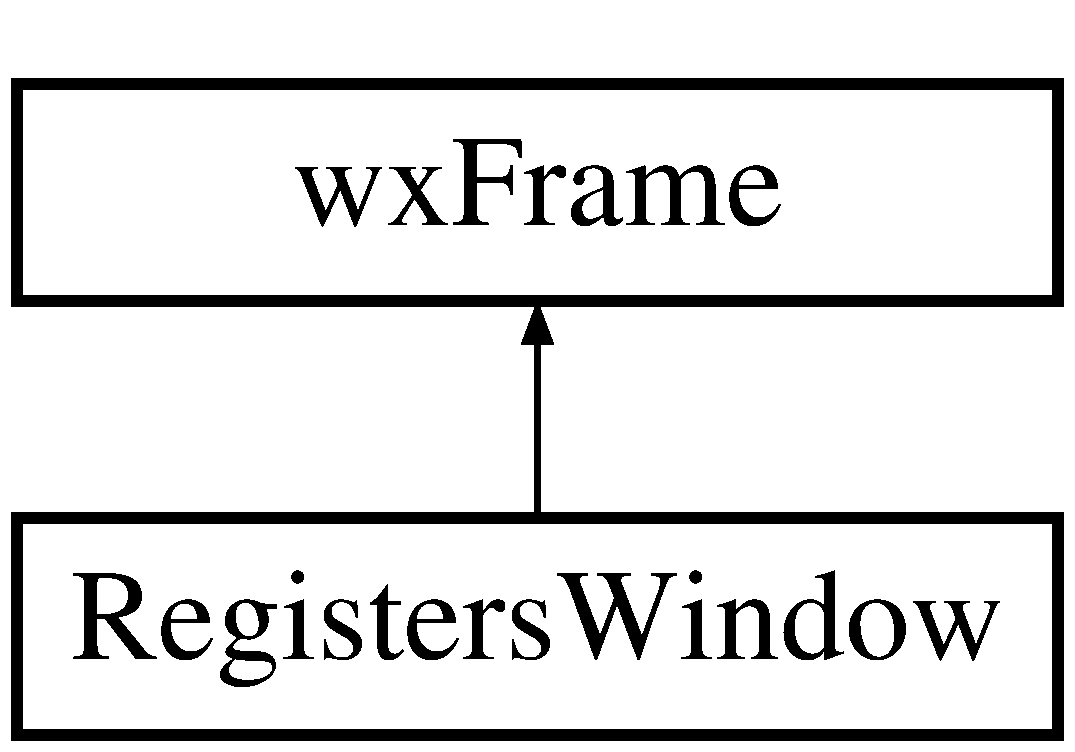
\includegraphics[height=2.000000cm]{class_registers_window}
\end{center}
\end{figure}
\subsection*{Public Member Functions}
\begin{DoxyCompactItemize}
\item 
\hyperlink{class_registers_window_a20e575990b7951158b38189730288421}{Registers\+Window} (wx\+Window $\ast$parent, const wx\+String \&title, const wx\+Point \&pos, const wx\+Size \&size)
\item 
\hyperlink{class_registers_window_a8218bf9cb1730e750c4c9ce8c6b92cfb}{$\sim$\+Registers\+Window} ()
\end{DoxyCompactItemize}
\subsection*{Public Attributes}
\begin{DoxyCompactItemize}
\item 
wx\+List\+Box $\ast$ \hyperlink{class_registers_window_a5d8baf6bde30c9782d102ed64816a3b3}{registers\+\_\+listbox} = N\+U\+LL
\end{DoxyCompactItemize}


\subsection{Constructor \& Destructor Documentation}
\mbox{\Hypertarget{class_registers_window_a20e575990b7951158b38189730288421}\label{class_registers_window_a20e575990b7951158b38189730288421}} 
\index{Registers\+Window@{Registers\+Window}!Registers\+Window@{Registers\+Window}}
\index{Registers\+Window@{Registers\+Window}!Registers\+Window@{Registers\+Window}}
\subsubsection{\texorpdfstring{Registers\+Window()}{RegistersWindow()}}
{\footnotesize\ttfamily Registers\+Window\+::\+Registers\+Window (\begin{DoxyParamCaption}\item[{wx\+Window $\ast$}]{parent,  }\item[{const wx\+String \&}]{title,  }\item[{const wx\+Point \&}]{pos,  }\item[{const wx\+Size \&}]{size }\end{DoxyParamCaption})}

\mbox{\Hypertarget{class_registers_window_a8218bf9cb1730e750c4c9ce8c6b92cfb}\label{class_registers_window_a8218bf9cb1730e750c4c9ce8c6b92cfb}} 
\index{Registers\+Window@{Registers\+Window}!````~Registers\+Window@{$\sim$\+Registers\+Window}}
\index{````~Registers\+Window@{$\sim$\+Registers\+Window}!Registers\+Window@{Registers\+Window}}
\subsubsection{\texorpdfstring{$\sim$\+Registers\+Window()}{~RegistersWindow()}}
{\footnotesize\ttfamily Registers\+Window\+::$\sim$\+Registers\+Window (\begin{DoxyParamCaption}{ }\end{DoxyParamCaption})}



\subsection{Member Data Documentation}
\mbox{\Hypertarget{class_registers_window_a5d8baf6bde30c9782d102ed64816a3b3}\label{class_registers_window_a5d8baf6bde30c9782d102ed64816a3b3}} 
\index{Registers\+Window@{Registers\+Window}!registers\+\_\+listbox@{registers\+\_\+listbox}}
\index{registers\+\_\+listbox@{registers\+\_\+listbox}!Registers\+Window@{Registers\+Window}}
\subsubsection{\texorpdfstring{registers\+\_\+listbox}{registers\_listbox}}
{\footnotesize\ttfamily wx\+List\+Box$\ast$ Registers\+Window\+::registers\+\_\+listbox = N\+U\+LL}



The documentation for this class was generated from the following files\+:\begin{DoxyCompactItemize}
\item 
include/\hyperlink{ultra64_8h}{ultra64.\+h}\item 
src/\hyperlink{ultra64_8cpp}{ultra64.\+cpp}\end{DoxyCompactItemize}

\hypertarget{classultra64_1_1_r_o_m}{}\section{ultra64\+:\+:R\+OM Class Reference}
\label{classultra64_1_1_r_o_m}\index{ultra64\+::\+R\+OM@{ultra64\+::\+R\+OM}}


{\ttfamily \#include $<$rom.\+h$>$}

\subsection*{Public Member Functions}
\begin{DoxyCompactItemize}
\item 
\hyperlink{classultra64_1_1_r_o_m_afd9900aa18e0fcc05739e4bff66781d2}{R\+OM} (std\+::string filename)
\item 
\hyperlink{classultra64_1_1_r_o_m_a4ac690b2e2d12bca1ae469580d4b5391}{$\sim$\+R\+OM} ()
\item 
unsigned char $\ast$ \hyperlink{classultra64_1_1_r_o_m_a6f4256c63403739183f9bd29c17903ad}{get\+\_\+pointer} ()
\item 
\hyperlink{structultra64_1_1_r_o_m__header}{R\+O\+M\+\_\+header} \hyperlink{classultra64_1_1_r_o_m_aa171df90056cfb47aabaee332a7b9290}{get\+\_\+header} ()
\item 
size\+\_\+t \hyperlink{classultra64_1_1_r_o_m_af623f78ee86889c872907a0434054506}{get\+\_\+size} ()
\end{DoxyCompactItemize}
\subsection*{Private Attributes}
\begin{DoxyCompactItemize}
\item 
size\+\_\+t \hyperlink{classultra64_1_1_r_o_m_a78f408d8ba2877e67d083268e912de18}{sz}
\item 
unsigned char $\ast$ \hyperlink{classultra64_1_1_r_o_m_a5853bb7a3ce6dbd099ee8477961394ec}{data}
\item 
\hyperlink{structultra64_1_1_r_o_m__header}{R\+O\+M\+\_\+header} \hyperlink{classultra64_1_1_r_o_m_a3d58a7b5227748040408010bcebd1a29}{header}
\end{DoxyCompactItemize}


\subsection{Constructor \& Destructor Documentation}
\mbox{\Hypertarget{classultra64_1_1_r_o_m_afd9900aa18e0fcc05739e4bff66781d2}\label{classultra64_1_1_r_o_m_afd9900aa18e0fcc05739e4bff66781d2}} 
\index{ultra64\+::\+R\+OM@{ultra64\+::\+R\+OM}!R\+OM@{R\+OM}}
\index{R\+OM@{R\+OM}!ultra64\+::\+R\+OM@{ultra64\+::\+R\+OM}}
\subsubsection{\texorpdfstring{R\+O\+M()}{ROM()}}
{\footnotesize\ttfamily ultra64\+::\+R\+O\+M\+::\+R\+OM (\begin{DoxyParamCaption}\item[{std\+::string}]{filename }\end{DoxyParamCaption})}

\mbox{\Hypertarget{classultra64_1_1_r_o_m_a4ac690b2e2d12bca1ae469580d4b5391}\label{classultra64_1_1_r_o_m_a4ac690b2e2d12bca1ae469580d4b5391}} 
\index{ultra64\+::\+R\+OM@{ultra64\+::\+R\+OM}!````~R\+OM@{$\sim$\+R\+OM}}
\index{````~R\+OM@{$\sim$\+R\+OM}!ultra64\+::\+R\+OM@{ultra64\+::\+R\+OM}}
\subsubsection{\texorpdfstring{$\sim$\+R\+O\+M()}{~ROM()}}
{\footnotesize\ttfamily ultra64\+::\+R\+O\+M\+::$\sim$\+R\+OM (\begin{DoxyParamCaption}{ }\end{DoxyParamCaption})}



\subsection{Member Function Documentation}
\mbox{\Hypertarget{classultra64_1_1_r_o_m_aa171df90056cfb47aabaee332a7b9290}\label{classultra64_1_1_r_o_m_aa171df90056cfb47aabaee332a7b9290}} 
\index{ultra64\+::\+R\+OM@{ultra64\+::\+R\+OM}!get\+\_\+header@{get\+\_\+header}}
\index{get\+\_\+header@{get\+\_\+header}!ultra64\+::\+R\+OM@{ultra64\+::\+R\+OM}}
\subsubsection{\texorpdfstring{get\+\_\+header()}{get\_header()}}
{\footnotesize\ttfamily \hyperlink{structultra64_1_1_r_o_m__header}{R\+O\+M\+\_\+header} ultra64\+::\+R\+O\+M\+::get\+\_\+header (\begin{DoxyParamCaption}{ }\end{DoxyParamCaption})}

\mbox{\Hypertarget{classultra64_1_1_r_o_m_a6f4256c63403739183f9bd29c17903ad}\label{classultra64_1_1_r_o_m_a6f4256c63403739183f9bd29c17903ad}} 
\index{ultra64\+::\+R\+OM@{ultra64\+::\+R\+OM}!get\+\_\+pointer@{get\+\_\+pointer}}
\index{get\+\_\+pointer@{get\+\_\+pointer}!ultra64\+::\+R\+OM@{ultra64\+::\+R\+OM}}
\subsubsection{\texorpdfstring{get\+\_\+pointer()}{get\_pointer()}}
{\footnotesize\ttfamily unsigned char $\ast$ ultra64\+::\+R\+O\+M\+::get\+\_\+pointer (\begin{DoxyParamCaption}{ }\end{DoxyParamCaption})}

\mbox{\Hypertarget{classultra64_1_1_r_o_m_af623f78ee86889c872907a0434054506}\label{classultra64_1_1_r_o_m_af623f78ee86889c872907a0434054506}} 
\index{ultra64\+::\+R\+OM@{ultra64\+::\+R\+OM}!get\+\_\+size@{get\+\_\+size}}
\index{get\+\_\+size@{get\+\_\+size}!ultra64\+::\+R\+OM@{ultra64\+::\+R\+OM}}
\subsubsection{\texorpdfstring{get\+\_\+size()}{get\_size()}}
{\footnotesize\ttfamily size\+\_\+t ultra64\+::\+R\+O\+M\+::get\+\_\+size (\begin{DoxyParamCaption}{ }\end{DoxyParamCaption})}



\subsection{Member Data Documentation}
\mbox{\Hypertarget{classultra64_1_1_r_o_m_a5853bb7a3ce6dbd099ee8477961394ec}\label{classultra64_1_1_r_o_m_a5853bb7a3ce6dbd099ee8477961394ec}} 
\index{ultra64\+::\+R\+OM@{ultra64\+::\+R\+OM}!data@{data}}
\index{data@{data}!ultra64\+::\+R\+OM@{ultra64\+::\+R\+OM}}
\subsubsection{\texorpdfstring{data}{data}}
{\footnotesize\ttfamily unsigned char$\ast$ ultra64\+::\+R\+O\+M\+::data\hspace{0.3cm}{\ttfamily [private]}}

\mbox{\Hypertarget{classultra64_1_1_r_o_m_a3d58a7b5227748040408010bcebd1a29}\label{classultra64_1_1_r_o_m_a3d58a7b5227748040408010bcebd1a29}} 
\index{ultra64\+::\+R\+OM@{ultra64\+::\+R\+OM}!header@{header}}
\index{header@{header}!ultra64\+::\+R\+OM@{ultra64\+::\+R\+OM}}
\subsubsection{\texorpdfstring{header}{header}}
{\footnotesize\ttfamily \hyperlink{structultra64_1_1_r_o_m__header}{R\+O\+M\+\_\+header} ultra64\+::\+R\+O\+M\+::header\hspace{0.3cm}{\ttfamily [private]}}

\mbox{\Hypertarget{classultra64_1_1_r_o_m_a78f408d8ba2877e67d083268e912de18}\label{classultra64_1_1_r_o_m_a78f408d8ba2877e67d083268e912de18}} 
\index{ultra64\+::\+R\+OM@{ultra64\+::\+R\+OM}!sz@{sz}}
\index{sz@{sz}!ultra64\+::\+R\+OM@{ultra64\+::\+R\+OM}}
\subsubsection{\texorpdfstring{sz}{sz}}
{\footnotesize\ttfamily size\+\_\+t ultra64\+::\+R\+O\+M\+::sz\hspace{0.3cm}{\ttfamily [private]}}



The documentation for this class was generated from the following files\+:\begin{DoxyCompactItemize}
\item 
include/\hyperlink{rom_8h}{rom.\+h}\item 
src/\hyperlink{rom_8cpp}{rom.\+cpp}\end{DoxyCompactItemize}

\hypertarget{structultra64_1_1_r_o_m__header}{}\section{ultra64\+:\+:R\+O\+M\+\_\+header Struct Reference}
\label{structultra64_1_1_r_o_m__header}\index{ultra64\+::\+R\+O\+M\+\_\+header@{ultra64\+::\+R\+O\+M\+\_\+header}}


{\ttfamily \#include $<$rom.\+h$>$}

\subsection*{Public Attributes}
\begin{DoxyCompactItemize}
\item 
uint16\+\_\+t \hyperlink{structultra64_1_1_r_o_m__header_ab207c693797be7e5788aa7f8bd6dbefa}{signature} = 0
\item 
uint32\+\_\+t \hyperlink{structultra64_1_1_r_o_m__header_a5b7b2660af49b9ce1362631d9ab70faa}{pc} = 0
\item 
uint16\+\_\+t \hyperlink{structultra64_1_1_r_o_m__header_a49c14b788c1df0a13e5b68f3cc642ac0}{country\+\_\+code} = 0
\item 
char \hyperlink{structultra64_1_1_r_o_m__header_a44c2a9d60543f704f83d078d5938ff59}{name} \mbox{[}27\mbox{]} = \{0\}
\end{DoxyCompactItemize}


\subsection{Member Data Documentation}
\mbox{\Hypertarget{structultra64_1_1_r_o_m__header_a49c14b788c1df0a13e5b68f3cc642ac0}\label{structultra64_1_1_r_o_m__header_a49c14b788c1df0a13e5b68f3cc642ac0}} 
\index{ultra64\+::\+R\+O\+M\+\_\+header@{ultra64\+::\+R\+O\+M\+\_\+header}!country\+\_\+code@{country\+\_\+code}}
\index{country\+\_\+code@{country\+\_\+code}!ultra64\+::\+R\+O\+M\+\_\+header@{ultra64\+::\+R\+O\+M\+\_\+header}}
\subsubsection{\texorpdfstring{country\+\_\+code}{country\_code}}
{\footnotesize\ttfamily uint16\+\_\+t ultra64\+::\+R\+O\+M\+\_\+header\+::country\+\_\+code = 0}

\mbox{\Hypertarget{structultra64_1_1_r_o_m__header_a44c2a9d60543f704f83d078d5938ff59}\label{structultra64_1_1_r_o_m__header_a44c2a9d60543f704f83d078d5938ff59}} 
\index{ultra64\+::\+R\+O\+M\+\_\+header@{ultra64\+::\+R\+O\+M\+\_\+header}!name@{name}}
\index{name@{name}!ultra64\+::\+R\+O\+M\+\_\+header@{ultra64\+::\+R\+O\+M\+\_\+header}}
\subsubsection{\texorpdfstring{name}{name}}
{\footnotesize\ttfamily char ultra64\+::\+R\+O\+M\+\_\+header\+::name\mbox{[}27\mbox{]} = \{0\}}

\mbox{\Hypertarget{structultra64_1_1_r_o_m__header_a5b7b2660af49b9ce1362631d9ab70faa}\label{structultra64_1_1_r_o_m__header_a5b7b2660af49b9ce1362631d9ab70faa}} 
\index{ultra64\+::\+R\+O\+M\+\_\+header@{ultra64\+::\+R\+O\+M\+\_\+header}!pc@{pc}}
\index{pc@{pc}!ultra64\+::\+R\+O\+M\+\_\+header@{ultra64\+::\+R\+O\+M\+\_\+header}}
\subsubsection{\texorpdfstring{pc}{pc}}
{\footnotesize\ttfamily uint32\+\_\+t ultra64\+::\+R\+O\+M\+\_\+header\+::pc = 0}

\mbox{\Hypertarget{structultra64_1_1_r_o_m__header_ab207c693797be7e5788aa7f8bd6dbefa}\label{structultra64_1_1_r_o_m__header_ab207c693797be7e5788aa7f8bd6dbefa}} 
\index{ultra64\+::\+R\+O\+M\+\_\+header@{ultra64\+::\+R\+O\+M\+\_\+header}!signature@{signature}}
\index{signature@{signature}!ultra64\+::\+R\+O\+M\+\_\+header@{ultra64\+::\+R\+O\+M\+\_\+header}}
\subsubsection{\texorpdfstring{signature}{signature}}
{\footnotesize\ttfamily uint16\+\_\+t ultra64\+::\+R\+O\+M\+\_\+header\+::signature = 0}



The documentation for this struct was generated from the following file\+:\begin{DoxyCompactItemize}
\item 
include/\hyperlink{rom_8h}{rom.\+h}\end{DoxyCompactItemize}

\hypertarget{classultra64_1_1rsp}{}\section{ultra64\+:\+:rsp Class Reference}
\label{classultra64_1_1rsp}\index{ultra64\+::rsp@{ultra64\+::rsp}}


{\ttfamily \#include $<$rsp.\+h$>$}

\subsection*{Public Member Functions}
\begin{DoxyCompactItemize}
\item 
\hyperlink{classultra64_1_1rsp_af573f798fee9c51b249bfe693689450c}{rsp} ()
\item 
\hyperlink{classultra64_1_1rsp_ac31547610349434e51969ed84c8c43ed}{$\sim$rsp} ()
\item 
void \hyperlink{classultra64_1_1rsp_a888d3e8dd8c86bbc512c6afed1922b9e}{step} ()
\end{DoxyCompactItemize}


\subsection{Constructor \& Destructor Documentation}
\mbox{\Hypertarget{classultra64_1_1rsp_af573f798fee9c51b249bfe693689450c}\label{classultra64_1_1rsp_af573f798fee9c51b249bfe693689450c}} 
\index{ultra64\+::rsp@{ultra64\+::rsp}!rsp@{rsp}}
\index{rsp@{rsp}!ultra64\+::rsp@{ultra64\+::rsp}}
\subsubsection{\texorpdfstring{rsp()}{rsp()}}
{\footnotesize\ttfamily ultra64\+::rsp\+::rsp (\begin{DoxyParamCaption}{ }\end{DoxyParamCaption})}

\mbox{\Hypertarget{classultra64_1_1rsp_ac31547610349434e51969ed84c8c43ed}\label{classultra64_1_1rsp_ac31547610349434e51969ed84c8c43ed}} 
\index{ultra64\+::rsp@{ultra64\+::rsp}!````~rsp@{$\sim$rsp}}
\index{````~rsp@{$\sim$rsp}!ultra64\+::rsp@{ultra64\+::rsp}}
\subsubsection{\texorpdfstring{$\sim$rsp()}{~rsp()}}
{\footnotesize\ttfamily ultra64\+::rsp\+::$\sim$rsp (\begin{DoxyParamCaption}{ }\end{DoxyParamCaption})}



\subsection{Member Function Documentation}
\mbox{\Hypertarget{classultra64_1_1rsp_a888d3e8dd8c86bbc512c6afed1922b9e}\label{classultra64_1_1rsp_a888d3e8dd8c86bbc512c6afed1922b9e}} 
\index{ultra64\+::rsp@{ultra64\+::rsp}!step@{step}}
\index{step@{step}!ultra64\+::rsp@{ultra64\+::rsp}}
\subsubsection{\texorpdfstring{step()}{step()}}
{\footnotesize\ttfamily void ultra64\+::rsp\+::step (\begin{DoxyParamCaption}{ }\end{DoxyParamCaption})}



The documentation for this class was generated from the following files\+:\begin{DoxyCompactItemize}
\item 
include/\hyperlink{rsp_8h}{rsp.\+h}\item 
src/rcp/\hyperlink{rsp_8cpp}{rsp.\+cpp}\end{DoxyCompactItemize}

\hypertarget{classwx_ultra64}{}\section{wx\+Ultra64 Class Reference}
\label{classwx_ultra64}\index{wx\+Ultra64@{wx\+Ultra64}}


{\ttfamily \#include $<$ultra64.\+h$>$}

Inheritance diagram for wx\+Ultra64\+:\begin{figure}[H]
\begin{center}
\leavevmode
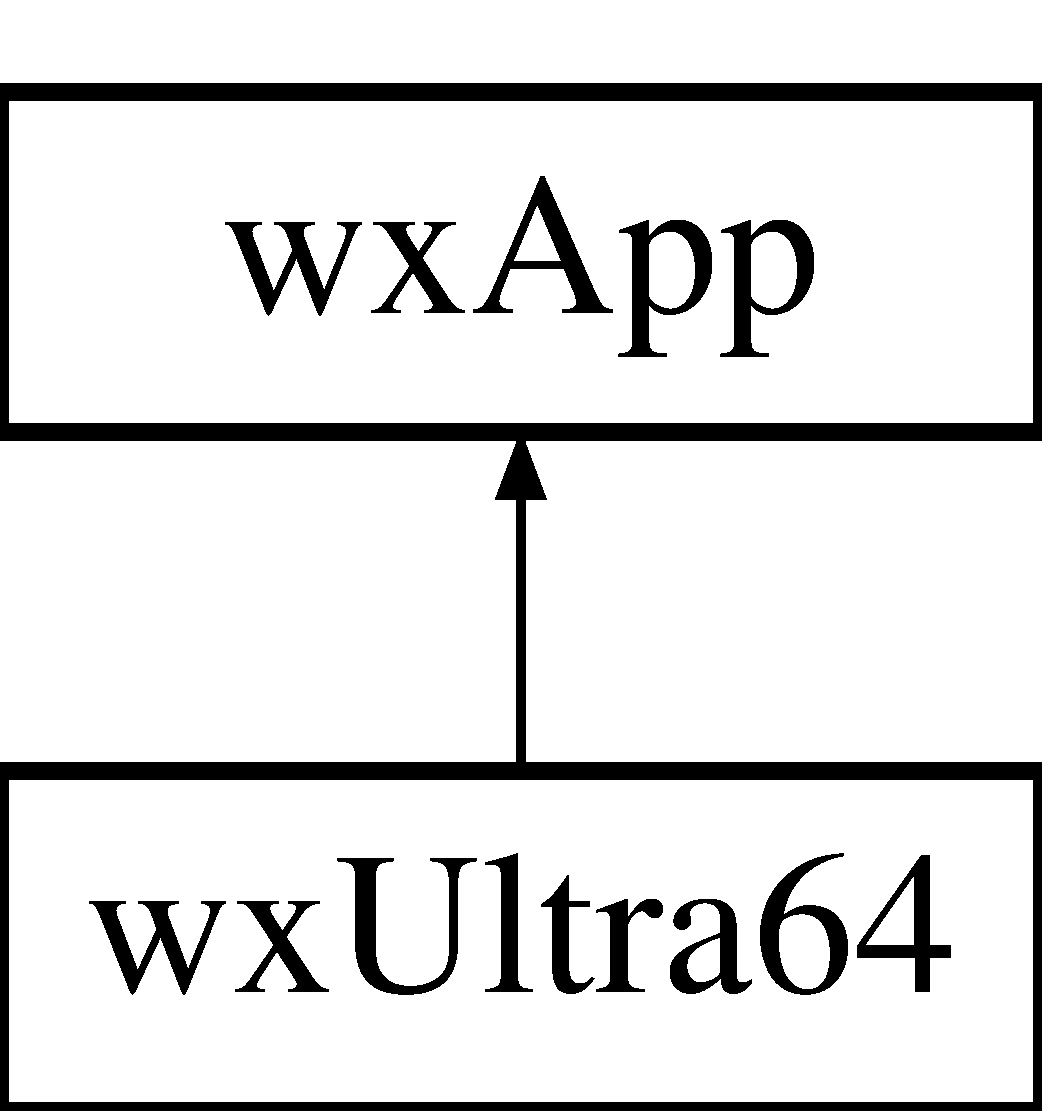
\includegraphics[height=2.000000cm]{classwx_ultra64}
\end{center}
\end{figure}
\subsection*{Public Member Functions}
\begin{DoxyCompactItemize}
\item 
virtual bool \hyperlink{classwx_ultra64_ac90ecee574b2aaeb016f34d46f5ca87d}{On\+Init} ()
\end{DoxyCompactItemize}
\subsection*{Public Attributes}
\begin{DoxyCompactItemize}
\item 
\hyperlink{class_main_window}{Main\+Window} $\ast$ \hyperlink{classwx_ultra64_a46b06489d6a269c6be154cb0a7e1e4e9}{frame} = N\+U\+LL
\item 
\hyperlink{class_debugger_window}{Debugger\+Window} $\ast$ \hyperlink{classwx_ultra64_ae2a892a46d0d8b8c2ff29a1b2d32133b}{debugger} = N\+U\+LL
\item 
\hyperlink{class_registers_window}{Registers\+Window} $\ast$ \hyperlink{classwx_ultra64_aa287d484fb611c20ef6f3b2c422b5e2c}{registers} = N\+U\+LL
\end{DoxyCompactItemize}


\subsection{Member Function Documentation}
\mbox{\Hypertarget{classwx_ultra64_ac90ecee574b2aaeb016f34d46f5ca87d}\label{classwx_ultra64_ac90ecee574b2aaeb016f34d46f5ca87d}} 
\index{wx\+Ultra64@{wx\+Ultra64}!On\+Init@{On\+Init}}
\index{On\+Init@{On\+Init}!wx\+Ultra64@{wx\+Ultra64}}
\subsubsection{\texorpdfstring{On\+Init()}{OnInit()}}
{\footnotesize\ttfamily bool wx\+Ultra64\+::\+On\+Init (\begin{DoxyParamCaption}{ }\end{DoxyParamCaption})\hspace{0.3cm}{\ttfamily [virtual]}}



\subsection{Member Data Documentation}
\mbox{\Hypertarget{classwx_ultra64_ae2a892a46d0d8b8c2ff29a1b2d32133b}\label{classwx_ultra64_ae2a892a46d0d8b8c2ff29a1b2d32133b}} 
\index{wx\+Ultra64@{wx\+Ultra64}!debugger@{debugger}}
\index{debugger@{debugger}!wx\+Ultra64@{wx\+Ultra64}}
\subsubsection{\texorpdfstring{debugger}{debugger}}
{\footnotesize\ttfamily \hyperlink{class_debugger_window}{Debugger\+Window}$\ast$ wx\+Ultra64\+::debugger = N\+U\+LL}

\mbox{\Hypertarget{classwx_ultra64_a46b06489d6a269c6be154cb0a7e1e4e9}\label{classwx_ultra64_a46b06489d6a269c6be154cb0a7e1e4e9}} 
\index{wx\+Ultra64@{wx\+Ultra64}!frame@{frame}}
\index{frame@{frame}!wx\+Ultra64@{wx\+Ultra64}}
\subsubsection{\texorpdfstring{frame}{frame}}
{\footnotesize\ttfamily \hyperlink{class_main_window}{Main\+Window}$\ast$ wx\+Ultra64\+::frame = N\+U\+LL}

\mbox{\Hypertarget{classwx_ultra64_aa287d484fb611c20ef6f3b2c422b5e2c}\label{classwx_ultra64_aa287d484fb611c20ef6f3b2c422b5e2c}} 
\index{wx\+Ultra64@{wx\+Ultra64}!registers@{registers}}
\index{registers@{registers}!wx\+Ultra64@{wx\+Ultra64}}
\subsubsection{\texorpdfstring{registers}{registers}}
{\footnotesize\ttfamily \hyperlink{class_registers_window}{Registers\+Window}$\ast$ wx\+Ultra64\+::registers = N\+U\+LL}



The documentation for this class was generated from the following files\+:\begin{DoxyCompactItemize}
\item 
include/\hyperlink{ultra64_8h}{ultra64.\+h}\item 
src/\hyperlink{ultra64_8cpp}{ultra64.\+cpp}\end{DoxyCompactItemize}

\chapter{File Documentation}
\hypertarget{config_8h}{}\section{config.\+h File Reference}
\label{config_8h}\index{config.\+h@{config.\+h}}
\subsection*{Macros}
\begin{DoxyCompactItemize}
\item 
\#define \hyperlink{config_8h_aca8570fb706c81df371b7f9bc454ae03}{P\+A\+C\+K\+A\+GE}~\char`\"{}ultra64\char`\"{}
\item 
\#define \hyperlink{config_8h_a1d1d2d7f8d2f95b376954d649ab03233}{P\+A\+C\+K\+A\+G\+E\+\_\+\+B\+U\+G\+R\+E\+P\+O\+RT}~\char`\"{}tim@metaverse.\+systems\char`\"{}
\item 
\#define \hyperlink{config_8h_a1c0439e4355794c09b64274849eb0279}{P\+A\+C\+K\+A\+G\+E\+\_\+\+N\+A\+ME}~\char`\"{}ultra64\char`\"{}
\item 
\#define \hyperlink{config_8h_ac73e6f903c16eca7710f92e36e1c6fbf}{P\+A\+C\+K\+A\+G\+E\+\_\+\+S\+T\+R\+I\+NG}~\char`\"{}ultra64 0.\+1\char`\"{}
\item 
\#define \hyperlink{config_8h_af415af6bfede0e8d5453708afe68651c}{P\+A\+C\+K\+A\+G\+E\+\_\+\+T\+A\+R\+N\+A\+ME}~\char`\"{}ultra64\char`\"{}
\item 
\#define \hyperlink{config_8h_a5c93853116d5a50307b6744f147840aa}{P\+A\+C\+K\+A\+G\+E\+\_\+\+U\+RL}~\char`\"{}\char`\"{}
\item 
\#define \hyperlink{config_8h_aa326a05d5e30f9e9a4bb0b4469d5d0c0}{P\+A\+C\+K\+A\+G\+E\+\_\+\+V\+E\+R\+S\+I\+ON}~\char`\"{}0.\+1\char`\"{}
\item 
\#define \hyperlink{config_8h_a1c6d5de492ac61ad29aec7aa9a436bbf}{V\+E\+R\+S\+I\+ON}~\char`\"{}0.\+1\char`\"{}
\end{DoxyCompactItemize}


\subsection{Macro Definition Documentation}
\mbox{\Hypertarget{config_8h_aca8570fb706c81df371b7f9bc454ae03}\label{config_8h_aca8570fb706c81df371b7f9bc454ae03}} 
\index{config.\+h@{config.\+h}!P\+A\+C\+K\+A\+GE@{P\+A\+C\+K\+A\+GE}}
\index{P\+A\+C\+K\+A\+GE@{P\+A\+C\+K\+A\+GE}!config.\+h@{config.\+h}}
\subsubsection{\texorpdfstring{P\+A\+C\+K\+A\+GE}{PACKAGE}}
{\footnotesize\ttfamily \#define P\+A\+C\+K\+A\+GE~\char`\"{}ultra64\char`\"{}}

\mbox{\Hypertarget{config_8h_a1d1d2d7f8d2f95b376954d649ab03233}\label{config_8h_a1d1d2d7f8d2f95b376954d649ab03233}} 
\index{config.\+h@{config.\+h}!P\+A\+C\+K\+A\+G\+E\+\_\+\+B\+U\+G\+R\+E\+P\+O\+RT@{P\+A\+C\+K\+A\+G\+E\+\_\+\+B\+U\+G\+R\+E\+P\+O\+RT}}
\index{P\+A\+C\+K\+A\+G\+E\+\_\+\+B\+U\+G\+R\+E\+P\+O\+RT@{P\+A\+C\+K\+A\+G\+E\+\_\+\+B\+U\+G\+R\+E\+P\+O\+RT}!config.\+h@{config.\+h}}
\subsubsection{\texorpdfstring{P\+A\+C\+K\+A\+G\+E\+\_\+\+B\+U\+G\+R\+E\+P\+O\+RT}{PACKAGE\_BUGREPORT}}
{\footnotesize\ttfamily \#define P\+A\+C\+K\+A\+G\+E\+\_\+\+B\+U\+G\+R\+E\+P\+O\+RT~\char`\"{}tim@metaverse.\+systems\char`\"{}}

\mbox{\Hypertarget{config_8h_a1c0439e4355794c09b64274849eb0279}\label{config_8h_a1c0439e4355794c09b64274849eb0279}} 
\index{config.\+h@{config.\+h}!P\+A\+C\+K\+A\+G\+E\+\_\+\+N\+A\+ME@{P\+A\+C\+K\+A\+G\+E\+\_\+\+N\+A\+ME}}
\index{P\+A\+C\+K\+A\+G\+E\+\_\+\+N\+A\+ME@{P\+A\+C\+K\+A\+G\+E\+\_\+\+N\+A\+ME}!config.\+h@{config.\+h}}
\subsubsection{\texorpdfstring{P\+A\+C\+K\+A\+G\+E\+\_\+\+N\+A\+ME}{PACKAGE\_NAME}}
{\footnotesize\ttfamily \#define P\+A\+C\+K\+A\+G\+E\+\_\+\+N\+A\+ME~\char`\"{}ultra64\char`\"{}}

\mbox{\Hypertarget{config_8h_ac73e6f903c16eca7710f92e36e1c6fbf}\label{config_8h_ac73e6f903c16eca7710f92e36e1c6fbf}} 
\index{config.\+h@{config.\+h}!P\+A\+C\+K\+A\+G\+E\+\_\+\+S\+T\+R\+I\+NG@{P\+A\+C\+K\+A\+G\+E\+\_\+\+S\+T\+R\+I\+NG}}
\index{P\+A\+C\+K\+A\+G\+E\+\_\+\+S\+T\+R\+I\+NG@{P\+A\+C\+K\+A\+G\+E\+\_\+\+S\+T\+R\+I\+NG}!config.\+h@{config.\+h}}
\subsubsection{\texorpdfstring{P\+A\+C\+K\+A\+G\+E\+\_\+\+S\+T\+R\+I\+NG}{PACKAGE\_STRING}}
{\footnotesize\ttfamily \#define P\+A\+C\+K\+A\+G\+E\+\_\+\+S\+T\+R\+I\+NG~\char`\"{}ultra64 0.\+1\char`\"{}}

\mbox{\Hypertarget{config_8h_af415af6bfede0e8d5453708afe68651c}\label{config_8h_af415af6bfede0e8d5453708afe68651c}} 
\index{config.\+h@{config.\+h}!P\+A\+C\+K\+A\+G\+E\+\_\+\+T\+A\+R\+N\+A\+ME@{P\+A\+C\+K\+A\+G\+E\+\_\+\+T\+A\+R\+N\+A\+ME}}
\index{P\+A\+C\+K\+A\+G\+E\+\_\+\+T\+A\+R\+N\+A\+ME@{P\+A\+C\+K\+A\+G\+E\+\_\+\+T\+A\+R\+N\+A\+ME}!config.\+h@{config.\+h}}
\subsubsection{\texorpdfstring{P\+A\+C\+K\+A\+G\+E\+\_\+\+T\+A\+R\+N\+A\+ME}{PACKAGE\_TARNAME}}
{\footnotesize\ttfamily \#define P\+A\+C\+K\+A\+G\+E\+\_\+\+T\+A\+R\+N\+A\+ME~\char`\"{}ultra64\char`\"{}}

\mbox{\Hypertarget{config_8h_a5c93853116d5a50307b6744f147840aa}\label{config_8h_a5c93853116d5a50307b6744f147840aa}} 
\index{config.\+h@{config.\+h}!P\+A\+C\+K\+A\+G\+E\+\_\+\+U\+RL@{P\+A\+C\+K\+A\+G\+E\+\_\+\+U\+RL}}
\index{P\+A\+C\+K\+A\+G\+E\+\_\+\+U\+RL@{P\+A\+C\+K\+A\+G\+E\+\_\+\+U\+RL}!config.\+h@{config.\+h}}
\subsubsection{\texorpdfstring{P\+A\+C\+K\+A\+G\+E\+\_\+\+U\+RL}{PACKAGE\_URL}}
{\footnotesize\ttfamily \#define P\+A\+C\+K\+A\+G\+E\+\_\+\+U\+RL~\char`\"{}\char`\"{}}

\mbox{\Hypertarget{config_8h_aa326a05d5e30f9e9a4bb0b4469d5d0c0}\label{config_8h_aa326a05d5e30f9e9a4bb0b4469d5d0c0}} 
\index{config.\+h@{config.\+h}!P\+A\+C\+K\+A\+G\+E\+\_\+\+V\+E\+R\+S\+I\+ON@{P\+A\+C\+K\+A\+G\+E\+\_\+\+V\+E\+R\+S\+I\+ON}}
\index{P\+A\+C\+K\+A\+G\+E\+\_\+\+V\+E\+R\+S\+I\+ON@{P\+A\+C\+K\+A\+G\+E\+\_\+\+V\+E\+R\+S\+I\+ON}!config.\+h@{config.\+h}}
\subsubsection{\texorpdfstring{P\+A\+C\+K\+A\+G\+E\+\_\+\+V\+E\+R\+S\+I\+ON}{PACKAGE\_VERSION}}
{\footnotesize\ttfamily \#define P\+A\+C\+K\+A\+G\+E\+\_\+\+V\+E\+R\+S\+I\+ON~\char`\"{}0.\+1\char`\"{}}

\mbox{\Hypertarget{config_8h_a1c6d5de492ac61ad29aec7aa9a436bbf}\label{config_8h_a1c6d5de492ac61ad29aec7aa9a436bbf}} 
\index{config.\+h@{config.\+h}!V\+E\+R\+S\+I\+ON@{V\+E\+R\+S\+I\+ON}}
\index{V\+E\+R\+S\+I\+ON@{V\+E\+R\+S\+I\+ON}!config.\+h@{config.\+h}}
\subsubsection{\texorpdfstring{V\+E\+R\+S\+I\+ON}{VERSION}}
{\footnotesize\ttfamily \#define V\+E\+R\+S\+I\+ON~\char`\"{}0.\+1\char`\"{}}


\hypertarget{memory_8h}{}\section{include/memory.h File Reference}
\label{memory_8h}\index{include/memory.\+h@{include/memory.\+h}}
{\ttfamily \#include $<$rom.\+h$>$}\newline
\subsection*{Classes}
\begin{DoxyCompactItemize}
\item 
struct \hyperlink{structultra64_1_1memory__section}{ultra64\+::memory\+\_\+section}
\item 
class \hyperlink{classultra64_1_1_m_m_u}{ultra64\+::\+M\+MU}
\end{DoxyCompactItemize}
\subsection*{Namespaces}
\begin{DoxyCompactItemize}
\item 
 \hyperlink{namespaceultra64}{ultra64}
\end{DoxyCompactItemize}
\subsection*{Variables}
\begin{DoxyCompactItemize}
\item 
\hyperlink{classultra64_1_1_m_m_u}{ultra64\+::\+M\+MU} $\ast$ \hyperlink{memory_8h_ad2faab063b0f86f630bf350495d65c18}{mmu}
\end{DoxyCompactItemize}


\subsection{Variable Documentation}
\mbox{\Hypertarget{memory_8h_ad2faab063b0f86f630bf350495d65c18}\label{memory_8h_ad2faab063b0f86f630bf350495d65c18}} 
\index{memory.\+h@{memory.\+h}!mmu@{mmu}}
\index{mmu@{mmu}!memory.\+h@{memory.\+h}}
\subsubsection{\texorpdfstring{mmu}{mmu}}
{\footnotesize\ttfamily \hyperlink{classultra64_1_1_m_m_u}{ultra64\+::\+M\+MU}$\ast$ mmu}


\hypertarget{opcodes_8h}{}\section{include/opcodes.h File Reference}
\label{opcodes_8h}\index{include/opcodes.\+h@{include/opcodes.\+h}}
\subsection*{Macros}
\begin{DoxyCompactItemize}
\item 
\#define \hyperlink{opcodes_8h_a71211ae8ec12566eecf5b66b13f426ad}{\+\_\+\+S\+P\+E\+C\+I\+AL}~0x00
\item 
\#define \hyperlink{opcodes_8h_a818251fd616b6bd271e9410a0f8119c9}{\+\_\+\+R\+E\+G\+I\+MM}~0x01
\item 
\#define \hyperlink{opcodes_8h_a9e21b1bbecbc6c491f4cb7de14e9b72c}{B\+EQ}~0x04
\item 
\#define \hyperlink{opcodes_8h_a4e557ce20e8f60bde33104f27f2f6f5d}{B\+NE}~0x05
\item 
\#define \hyperlink{opcodes_8h_a240067f241bac82304fe36d2d4a296da}{A\+D\+DI}~0x08
\item 
\#define \hyperlink{opcodes_8h_a1e15de33589a110fadf1bdd5ef0586ed}{A\+D\+D\+IU}~0x09
\item 
\#define \hyperlink{opcodes_8h_a6629468bc5e11d36efed350908f2dff4}{A\+N\+DI}~0x0C
\item 
\#define \hyperlink{opcodes_8h_ade8154dab9666f65904be28a9e4cadb5}{O\+RI}~0x0D
\item 
\#define \hyperlink{opcodes_8h_ae253f17e1792a8324699cdaca73cf387}{L\+UI}~0x0F
\item 
\#define \hyperlink{opcodes_8h_aeda5d5cf7f38aeaa0184906d715d5b78}{\+\_\+\+C\+P0}~0x10
\item 
\#define \hyperlink{opcodes_8h_a6cb54da41e2cf60c33f27c01d831fb86}{B\+E\+QL}~0x14
\item 
\#define \hyperlink{opcodes_8h_a677c0f7a675fb4c6ba0d2cb0ea1339ef}{B\+N\+EL}~0x15
\item 
\#define \hyperlink{opcodes_8h_a990908478ddb516854fbbc0ad39a1210}{D\+A\+D\+DI}~0x18
\item 
\#define \hyperlink{opcodes_8h_acc55daa58d88a3612f2ef74a6abbe97f}{LB}~0x20
\item 
\#define \hyperlink{opcodes_8h_ad4b135b7ba4889a823f26261d8de74b3}{LW}~0x23
\item 
\#define \hyperlink{opcodes_8h_a4b95e941f44a20ea60512bbe2065f0b6}{SW}~0x2B
\item 
\#define \hyperlink{opcodes_8h_a189dc429a87af5f7abf3c53b32d7889b}{S\+LL}~0x00
\item 
\#define \hyperlink{opcodes_8h_a391959af0568008f17f41df83486de19}{S\+RL}~0x02
\item 
\#define \hyperlink{opcodes_8h_a88c66bd83a52f8af1b3c9d5e092b6052}{S\+L\+LV}~0x04
\item 
\#define \hyperlink{opcodes_8h_acca016f684440550f9b9afbbdca9ed5f}{S\+R\+LV}~0x06
\item 
\#define \hyperlink{opcodes_8h_a2be408601f1de958fd6243bd97efe40f}{JR}~0x08
\item 
\#define \hyperlink{opcodes_8h_ad4061310dc88d6c556cfb91cb278ae05}{M\+F\+HI}~0x10
\item 
\#define \hyperlink{opcodes_8h_a2c5fb79d0480b74c1fedf37affed197c}{M\+F\+LO}~0x12
\item 
\#define \hyperlink{opcodes_8h_a373b30f48f584a543bd869652eb34225}{M\+U\+L\+TU}~0x19
\item 
\#define \hyperlink{opcodes_8h_a6eced4f7caed8b9b31bcebd0209a8314}{A\+D\+DU}~0x21
\item 
\#define \hyperlink{opcodes_8h_a90ec3d1c2c662135c26210b78a472d56}{S\+U\+BU}~0x23
\item 
\#define \hyperlink{opcodes_8h_acd1b97556dfbbac61063a63031d2f91d}{A\+ND}~0x24
\item 
\#define \hyperlink{opcodes_8h_a3363ca4d6d3cc0230b2804280591c991}{OR}~0x25
\item 
\#define \hyperlink{opcodes_8h_a45cd11034d1a7d86c3a88d36f5e7f1ab}{X\+OR}~0x26
\item 
\#define \hyperlink{opcodes_8h_afedbd56796babcf8aab4442d0d962c08}{S\+L\+TU}~0x2B
\item 
\#define \hyperlink{opcodes_8h_a7c989c4ba408f9185e920f7c8fec083b}{D\+S\+L\+L32}~0x3C
\item 
\#define \hyperlink{opcodes_8h_a5d895cc559f9e84bec737efdc5657284}{B\+L\+TZ}~0x00
\item 
\#define \hyperlink{opcodes_8h_a376093e92e67d1e698a5fdd7a58e5069}{B\+G\+E\+Z\+AL}~0x11
\item 
\#define \hyperlink{opcodes_8h_a13d1731c920850917c3031bf7303539e}{M\+F\+C0}~0x00
\item 
\#define \hyperlink{opcodes_8h_ab7ca9eb5a776884fec2120f67412c9c2}{M\+T\+C0}~0x04
\end{DoxyCompactItemize}


\subsection{Macro Definition Documentation}
\mbox{\Hypertarget{opcodes_8h_aeda5d5cf7f38aeaa0184906d715d5b78}\label{opcodes_8h_aeda5d5cf7f38aeaa0184906d715d5b78}} 
\index{opcodes.\+h@{opcodes.\+h}!\+\_\+\+C\+P0@{\+\_\+\+C\+P0}}
\index{\+\_\+\+C\+P0@{\+\_\+\+C\+P0}!opcodes.\+h@{opcodes.\+h}}
\subsubsection{\texorpdfstring{\+\_\+\+C\+P0}{\_CP0}}
{\footnotesize\ttfamily \#define \+\_\+\+C\+P0~0x10}

\mbox{\Hypertarget{opcodes_8h_a818251fd616b6bd271e9410a0f8119c9}\label{opcodes_8h_a818251fd616b6bd271e9410a0f8119c9}} 
\index{opcodes.\+h@{opcodes.\+h}!\+\_\+\+R\+E\+G\+I\+MM@{\+\_\+\+R\+E\+G\+I\+MM}}
\index{\+\_\+\+R\+E\+G\+I\+MM@{\+\_\+\+R\+E\+G\+I\+MM}!opcodes.\+h@{opcodes.\+h}}
\subsubsection{\texorpdfstring{\+\_\+\+R\+E\+G\+I\+MM}{\_REGIMM}}
{\footnotesize\ttfamily \#define \+\_\+\+R\+E\+G\+I\+MM~0x01}

\mbox{\Hypertarget{opcodes_8h_a71211ae8ec12566eecf5b66b13f426ad}\label{opcodes_8h_a71211ae8ec12566eecf5b66b13f426ad}} 
\index{opcodes.\+h@{opcodes.\+h}!\+\_\+\+S\+P\+E\+C\+I\+AL@{\+\_\+\+S\+P\+E\+C\+I\+AL}}
\index{\+\_\+\+S\+P\+E\+C\+I\+AL@{\+\_\+\+S\+P\+E\+C\+I\+AL}!opcodes.\+h@{opcodes.\+h}}
\subsubsection{\texorpdfstring{\+\_\+\+S\+P\+E\+C\+I\+AL}{\_SPECIAL}}
{\footnotesize\ttfamily \#define \+\_\+\+S\+P\+E\+C\+I\+AL~0x00}

\mbox{\Hypertarget{opcodes_8h_a240067f241bac82304fe36d2d4a296da}\label{opcodes_8h_a240067f241bac82304fe36d2d4a296da}} 
\index{opcodes.\+h@{opcodes.\+h}!A\+D\+DI@{A\+D\+DI}}
\index{A\+D\+DI@{A\+D\+DI}!opcodes.\+h@{opcodes.\+h}}
\subsubsection{\texorpdfstring{A\+D\+DI}{ADDI}}
{\footnotesize\ttfamily \#define A\+D\+DI~0x08}

\mbox{\Hypertarget{opcodes_8h_a1e15de33589a110fadf1bdd5ef0586ed}\label{opcodes_8h_a1e15de33589a110fadf1bdd5ef0586ed}} 
\index{opcodes.\+h@{opcodes.\+h}!A\+D\+D\+IU@{A\+D\+D\+IU}}
\index{A\+D\+D\+IU@{A\+D\+D\+IU}!opcodes.\+h@{opcodes.\+h}}
\subsubsection{\texorpdfstring{A\+D\+D\+IU}{ADDIU}}
{\footnotesize\ttfamily \#define A\+D\+D\+IU~0x09}

\mbox{\Hypertarget{opcodes_8h_a6eced4f7caed8b9b31bcebd0209a8314}\label{opcodes_8h_a6eced4f7caed8b9b31bcebd0209a8314}} 
\index{opcodes.\+h@{opcodes.\+h}!A\+D\+DU@{A\+D\+DU}}
\index{A\+D\+DU@{A\+D\+DU}!opcodes.\+h@{opcodes.\+h}}
\subsubsection{\texorpdfstring{A\+D\+DU}{ADDU}}
{\footnotesize\ttfamily \#define A\+D\+DU~0x21}

\mbox{\Hypertarget{opcodes_8h_acd1b97556dfbbac61063a63031d2f91d}\label{opcodes_8h_acd1b97556dfbbac61063a63031d2f91d}} 
\index{opcodes.\+h@{opcodes.\+h}!A\+ND@{A\+ND}}
\index{A\+ND@{A\+ND}!opcodes.\+h@{opcodes.\+h}}
\subsubsection{\texorpdfstring{A\+ND}{AND}}
{\footnotesize\ttfamily \#define A\+ND~0x24}

\mbox{\Hypertarget{opcodes_8h_a6629468bc5e11d36efed350908f2dff4}\label{opcodes_8h_a6629468bc5e11d36efed350908f2dff4}} 
\index{opcodes.\+h@{opcodes.\+h}!A\+N\+DI@{A\+N\+DI}}
\index{A\+N\+DI@{A\+N\+DI}!opcodes.\+h@{opcodes.\+h}}
\subsubsection{\texorpdfstring{A\+N\+DI}{ANDI}}
{\footnotesize\ttfamily \#define A\+N\+DI~0x0C}

\mbox{\Hypertarget{opcodes_8h_a9e21b1bbecbc6c491f4cb7de14e9b72c}\label{opcodes_8h_a9e21b1bbecbc6c491f4cb7de14e9b72c}} 
\index{opcodes.\+h@{opcodes.\+h}!B\+EQ@{B\+EQ}}
\index{B\+EQ@{B\+EQ}!opcodes.\+h@{opcodes.\+h}}
\subsubsection{\texorpdfstring{B\+EQ}{BEQ}}
{\footnotesize\ttfamily \#define B\+EQ~0x04}

\mbox{\Hypertarget{opcodes_8h_a6cb54da41e2cf60c33f27c01d831fb86}\label{opcodes_8h_a6cb54da41e2cf60c33f27c01d831fb86}} 
\index{opcodes.\+h@{opcodes.\+h}!B\+E\+QL@{B\+E\+QL}}
\index{B\+E\+QL@{B\+E\+QL}!opcodes.\+h@{opcodes.\+h}}
\subsubsection{\texorpdfstring{B\+E\+QL}{BEQL}}
{\footnotesize\ttfamily \#define B\+E\+QL~0x14}

\mbox{\Hypertarget{opcodes_8h_a376093e92e67d1e698a5fdd7a58e5069}\label{opcodes_8h_a376093e92e67d1e698a5fdd7a58e5069}} 
\index{opcodes.\+h@{opcodes.\+h}!B\+G\+E\+Z\+AL@{B\+G\+E\+Z\+AL}}
\index{B\+G\+E\+Z\+AL@{B\+G\+E\+Z\+AL}!opcodes.\+h@{opcodes.\+h}}
\subsubsection{\texorpdfstring{B\+G\+E\+Z\+AL}{BGEZAL}}
{\footnotesize\ttfamily \#define B\+G\+E\+Z\+AL~0x11}

\mbox{\Hypertarget{opcodes_8h_a5d895cc559f9e84bec737efdc5657284}\label{opcodes_8h_a5d895cc559f9e84bec737efdc5657284}} 
\index{opcodes.\+h@{opcodes.\+h}!B\+L\+TZ@{B\+L\+TZ}}
\index{B\+L\+TZ@{B\+L\+TZ}!opcodes.\+h@{opcodes.\+h}}
\subsubsection{\texorpdfstring{B\+L\+TZ}{BLTZ}}
{\footnotesize\ttfamily \#define B\+L\+TZ~0x00}

\mbox{\Hypertarget{opcodes_8h_a4e557ce20e8f60bde33104f27f2f6f5d}\label{opcodes_8h_a4e557ce20e8f60bde33104f27f2f6f5d}} 
\index{opcodes.\+h@{opcodes.\+h}!B\+NE@{B\+NE}}
\index{B\+NE@{B\+NE}!opcodes.\+h@{opcodes.\+h}}
\subsubsection{\texorpdfstring{B\+NE}{BNE}}
{\footnotesize\ttfamily \#define B\+NE~0x05}

\mbox{\Hypertarget{opcodes_8h_a677c0f7a675fb4c6ba0d2cb0ea1339ef}\label{opcodes_8h_a677c0f7a675fb4c6ba0d2cb0ea1339ef}} 
\index{opcodes.\+h@{opcodes.\+h}!B\+N\+EL@{B\+N\+EL}}
\index{B\+N\+EL@{B\+N\+EL}!opcodes.\+h@{opcodes.\+h}}
\subsubsection{\texorpdfstring{B\+N\+EL}{BNEL}}
{\footnotesize\ttfamily \#define B\+N\+EL~0x15}

\mbox{\Hypertarget{opcodes_8h_a990908478ddb516854fbbc0ad39a1210}\label{opcodes_8h_a990908478ddb516854fbbc0ad39a1210}} 
\index{opcodes.\+h@{opcodes.\+h}!D\+A\+D\+DI@{D\+A\+D\+DI}}
\index{D\+A\+D\+DI@{D\+A\+D\+DI}!opcodes.\+h@{opcodes.\+h}}
\subsubsection{\texorpdfstring{D\+A\+D\+DI}{DADDI}}
{\footnotesize\ttfamily \#define D\+A\+D\+DI~0x18}

\mbox{\Hypertarget{opcodes_8h_a7c989c4ba408f9185e920f7c8fec083b}\label{opcodes_8h_a7c989c4ba408f9185e920f7c8fec083b}} 
\index{opcodes.\+h@{opcodes.\+h}!D\+S\+L\+L32@{D\+S\+L\+L32}}
\index{D\+S\+L\+L32@{D\+S\+L\+L32}!opcodes.\+h@{opcodes.\+h}}
\subsubsection{\texorpdfstring{D\+S\+L\+L32}{DSLL32}}
{\footnotesize\ttfamily \#define D\+S\+L\+L32~0x3C}

\mbox{\Hypertarget{opcodes_8h_a2be408601f1de958fd6243bd97efe40f}\label{opcodes_8h_a2be408601f1de958fd6243bd97efe40f}} 
\index{opcodes.\+h@{opcodes.\+h}!JR@{JR}}
\index{JR@{JR}!opcodes.\+h@{opcodes.\+h}}
\subsubsection{\texorpdfstring{JR}{JR}}
{\footnotesize\ttfamily \#define JR~0x08}

\mbox{\Hypertarget{opcodes_8h_acc55daa58d88a3612f2ef74a6abbe97f}\label{opcodes_8h_acc55daa58d88a3612f2ef74a6abbe97f}} 
\index{opcodes.\+h@{opcodes.\+h}!LB@{LB}}
\index{LB@{LB}!opcodes.\+h@{opcodes.\+h}}
\subsubsection{\texorpdfstring{LB}{LB}}
{\footnotesize\ttfamily \#define LB~0x20}

\mbox{\Hypertarget{opcodes_8h_ae253f17e1792a8324699cdaca73cf387}\label{opcodes_8h_ae253f17e1792a8324699cdaca73cf387}} 
\index{opcodes.\+h@{opcodes.\+h}!L\+UI@{L\+UI}}
\index{L\+UI@{L\+UI}!opcodes.\+h@{opcodes.\+h}}
\subsubsection{\texorpdfstring{L\+UI}{LUI}}
{\footnotesize\ttfamily \#define L\+UI~0x0F}

\mbox{\Hypertarget{opcodes_8h_ad4b135b7ba4889a823f26261d8de74b3}\label{opcodes_8h_ad4b135b7ba4889a823f26261d8de74b3}} 
\index{opcodes.\+h@{opcodes.\+h}!LW@{LW}}
\index{LW@{LW}!opcodes.\+h@{opcodes.\+h}}
\subsubsection{\texorpdfstring{LW}{LW}}
{\footnotesize\ttfamily \#define LW~0x23}

\mbox{\Hypertarget{opcodes_8h_a13d1731c920850917c3031bf7303539e}\label{opcodes_8h_a13d1731c920850917c3031bf7303539e}} 
\index{opcodes.\+h@{opcodes.\+h}!M\+F\+C0@{M\+F\+C0}}
\index{M\+F\+C0@{M\+F\+C0}!opcodes.\+h@{opcodes.\+h}}
\subsubsection{\texorpdfstring{M\+F\+C0}{MFC0}}
{\footnotesize\ttfamily \#define M\+F\+C0~0x00}

\mbox{\Hypertarget{opcodes_8h_ad4061310dc88d6c556cfb91cb278ae05}\label{opcodes_8h_ad4061310dc88d6c556cfb91cb278ae05}} 
\index{opcodes.\+h@{opcodes.\+h}!M\+F\+HI@{M\+F\+HI}}
\index{M\+F\+HI@{M\+F\+HI}!opcodes.\+h@{opcodes.\+h}}
\subsubsection{\texorpdfstring{M\+F\+HI}{MFHI}}
{\footnotesize\ttfamily \#define M\+F\+HI~0x10}

\mbox{\Hypertarget{opcodes_8h_a2c5fb79d0480b74c1fedf37affed197c}\label{opcodes_8h_a2c5fb79d0480b74c1fedf37affed197c}} 
\index{opcodes.\+h@{opcodes.\+h}!M\+F\+LO@{M\+F\+LO}}
\index{M\+F\+LO@{M\+F\+LO}!opcodes.\+h@{opcodes.\+h}}
\subsubsection{\texorpdfstring{M\+F\+LO}{MFLO}}
{\footnotesize\ttfamily \#define M\+F\+LO~0x12}

\mbox{\Hypertarget{opcodes_8h_ab7ca9eb5a776884fec2120f67412c9c2}\label{opcodes_8h_ab7ca9eb5a776884fec2120f67412c9c2}} 
\index{opcodes.\+h@{opcodes.\+h}!M\+T\+C0@{M\+T\+C0}}
\index{M\+T\+C0@{M\+T\+C0}!opcodes.\+h@{opcodes.\+h}}
\subsubsection{\texorpdfstring{M\+T\+C0}{MTC0}}
{\footnotesize\ttfamily \#define M\+T\+C0~0x04}

\mbox{\Hypertarget{opcodes_8h_a373b30f48f584a543bd869652eb34225}\label{opcodes_8h_a373b30f48f584a543bd869652eb34225}} 
\index{opcodes.\+h@{opcodes.\+h}!M\+U\+L\+TU@{M\+U\+L\+TU}}
\index{M\+U\+L\+TU@{M\+U\+L\+TU}!opcodes.\+h@{opcodes.\+h}}
\subsubsection{\texorpdfstring{M\+U\+L\+TU}{MULTU}}
{\footnotesize\ttfamily \#define M\+U\+L\+TU~0x19}

\mbox{\Hypertarget{opcodes_8h_a3363ca4d6d3cc0230b2804280591c991}\label{opcodes_8h_a3363ca4d6d3cc0230b2804280591c991}} 
\index{opcodes.\+h@{opcodes.\+h}!OR@{OR}}
\index{OR@{OR}!opcodes.\+h@{opcodes.\+h}}
\subsubsection{\texorpdfstring{OR}{OR}}
{\footnotesize\ttfamily \#define OR~0x25}

\mbox{\Hypertarget{opcodes_8h_ade8154dab9666f65904be28a9e4cadb5}\label{opcodes_8h_ade8154dab9666f65904be28a9e4cadb5}} 
\index{opcodes.\+h@{opcodes.\+h}!O\+RI@{O\+RI}}
\index{O\+RI@{O\+RI}!opcodes.\+h@{opcodes.\+h}}
\subsubsection{\texorpdfstring{O\+RI}{ORI}}
{\footnotesize\ttfamily \#define O\+RI~0x0D}

\mbox{\Hypertarget{opcodes_8h_a189dc429a87af5f7abf3c53b32d7889b}\label{opcodes_8h_a189dc429a87af5f7abf3c53b32d7889b}} 
\index{opcodes.\+h@{opcodes.\+h}!S\+LL@{S\+LL}}
\index{S\+LL@{S\+LL}!opcodes.\+h@{opcodes.\+h}}
\subsubsection{\texorpdfstring{S\+LL}{SLL}}
{\footnotesize\ttfamily \#define S\+LL~0x00}

\mbox{\Hypertarget{opcodes_8h_a88c66bd83a52f8af1b3c9d5e092b6052}\label{opcodes_8h_a88c66bd83a52f8af1b3c9d5e092b6052}} 
\index{opcodes.\+h@{opcodes.\+h}!S\+L\+LV@{S\+L\+LV}}
\index{S\+L\+LV@{S\+L\+LV}!opcodes.\+h@{opcodes.\+h}}
\subsubsection{\texorpdfstring{S\+L\+LV}{SLLV}}
{\footnotesize\ttfamily \#define S\+L\+LV~0x04}

\mbox{\Hypertarget{opcodes_8h_afedbd56796babcf8aab4442d0d962c08}\label{opcodes_8h_afedbd56796babcf8aab4442d0d962c08}} 
\index{opcodes.\+h@{opcodes.\+h}!S\+L\+TU@{S\+L\+TU}}
\index{S\+L\+TU@{S\+L\+TU}!opcodes.\+h@{opcodes.\+h}}
\subsubsection{\texorpdfstring{S\+L\+TU}{SLTU}}
{\footnotesize\ttfamily \#define S\+L\+TU~0x2B}

\mbox{\Hypertarget{opcodes_8h_a391959af0568008f17f41df83486de19}\label{opcodes_8h_a391959af0568008f17f41df83486de19}} 
\index{opcodes.\+h@{opcodes.\+h}!S\+RL@{S\+RL}}
\index{S\+RL@{S\+RL}!opcodes.\+h@{opcodes.\+h}}
\subsubsection{\texorpdfstring{S\+RL}{SRL}}
{\footnotesize\ttfamily \#define S\+RL~0x02}

\mbox{\Hypertarget{opcodes_8h_acca016f684440550f9b9afbbdca9ed5f}\label{opcodes_8h_acca016f684440550f9b9afbbdca9ed5f}} 
\index{opcodes.\+h@{opcodes.\+h}!S\+R\+LV@{S\+R\+LV}}
\index{S\+R\+LV@{S\+R\+LV}!opcodes.\+h@{opcodes.\+h}}
\subsubsection{\texorpdfstring{S\+R\+LV}{SRLV}}
{\footnotesize\ttfamily \#define S\+R\+LV~0x06}

\mbox{\Hypertarget{opcodes_8h_a90ec3d1c2c662135c26210b78a472d56}\label{opcodes_8h_a90ec3d1c2c662135c26210b78a472d56}} 
\index{opcodes.\+h@{opcodes.\+h}!S\+U\+BU@{S\+U\+BU}}
\index{S\+U\+BU@{S\+U\+BU}!opcodes.\+h@{opcodes.\+h}}
\subsubsection{\texorpdfstring{S\+U\+BU}{SUBU}}
{\footnotesize\ttfamily \#define S\+U\+BU~0x23}

\mbox{\Hypertarget{opcodes_8h_a4b95e941f44a20ea60512bbe2065f0b6}\label{opcodes_8h_a4b95e941f44a20ea60512bbe2065f0b6}} 
\index{opcodes.\+h@{opcodes.\+h}!SW@{SW}}
\index{SW@{SW}!opcodes.\+h@{opcodes.\+h}}
\subsubsection{\texorpdfstring{SW}{SW}}
{\footnotesize\ttfamily \#define SW~0x2B}

\mbox{\Hypertarget{opcodes_8h_a45cd11034d1a7d86c3a88d36f5e7f1ab}\label{opcodes_8h_a45cd11034d1a7d86c3a88d36f5e7f1ab}} 
\index{opcodes.\+h@{opcodes.\+h}!X\+OR@{X\+OR}}
\index{X\+OR@{X\+OR}!opcodes.\+h@{opcodes.\+h}}
\subsubsection{\texorpdfstring{X\+OR}{XOR}}
{\footnotesize\ttfamily \#define X\+OR~0x26}


\hypertarget{pif__rom_8h}{}\section{include/pif\+\_\+rom.h File Reference}
\label{pif__rom_8h}\index{include/pif\+\_\+rom.\+h@{include/pif\+\_\+rom.\+h}}
{\ttfamily \#include $<$string$>$}\newline
\subsection*{Classes}
\begin{DoxyCompactItemize}
\item 
class \hyperlink{classultra64_1_1_p_i_f___r_o_m}{ultra64\+::\+P\+I\+F\+\_\+\+R\+OM}
\end{DoxyCompactItemize}
\subsection*{Namespaces}
\begin{DoxyCompactItemize}
\item 
 \hyperlink{namespaceultra64}{ultra64}
\end{DoxyCompactItemize}

\hypertarget{r4300_8h}{}\section{include/r4300.h File Reference}
\label{r4300_8h}\index{include/r4300.\+h@{include/r4300.\+h}}
{\ttfamily \#include $<$cstdint$>$}\newline
{\ttfamily \#include $<$unordered\+\_\+map$>$}\newline
{\ttfamily \#include $<$memory.\+h$>$}\newline
{\ttfamily \#include $<$opcodes.\+h$>$}\newline
\subsection*{Classes}
\begin{DoxyCompactItemize}
\item 
class \hyperlink{classultra64_1_1opcode__t}{ultra64\+::opcode\+\_\+t}
\item 
class \hyperlink{classultra64_1_1r4300}{ultra64\+::r4300}
\end{DoxyCompactItemize}
\subsection*{Namespaces}
\begin{DoxyCompactItemize}
\item 
 \hyperlink{namespaceultra64}{ultra64}
\end{DoxyCompactItemize}
\subsection*{Macros}
\begin{DoxyCompactItemize}
\item 
\#define \hyperlink{r4300_8h_a7609ee748f35b94cb6013fe98fbff67c}{\+\_\+\+U\+L\+T\+R\+A64\+\_\+\+R4300\+\_\+h}
\end{DoxyCompactItemize}


\subsection{Macro Definition Documentation}
\mbox{\Hypertarget{r4300_8h_a7609ee748f35b94cb6013fe98fbff67c}\label{r4300_8h_a7609ee748f35b94cb6013fe98fbff67c}} 
\index{r4300.\+h@{r4300.\+h}!\+\_\+\+U\+L\+T\+R\+A64\+\_\+\+R4300\+\_\+h@{\+\_\+\+U\+L\+T\+R\+A64\+\_\+\+R4300\+\_\+h}}
\index{\+\_\+\+U\+L\+T\+R\+A64\+\_\+\+R4300\+\_\+h@{\+\_\+\+U\+L\+T\+R\+A64\+\_\+\+R4300\+\_\+h}!r4300.\+h@{r4300.\+h}}
\subsubsection{\texorpdfstring{\+\_\+\+U\+L\+T\+R\+A64\+\_\+\+R4300\+\_\+h}{\_ULTRA64\_R4300\_h}}
{\footnotesize\ttfamily \#define \+\_\+\+U\+L\+T\+R\+A64\+\_\+\+R4300\+\_\+h}


\hypertarget{rom_8h}{}\section{include/rom.h File Reference}
\label{rom_8h}\index{include/rom.\+h@{include/rom.\+h}}
{\ttfamily \#include $<$string$>$}\newline
\subsection*{Classes}
\begin{DoxyCompactItemize}
\item 
struct \hyperlink{structultra64_1_1_r_o_m__header}{ultra64\+::\+R\+O\+M\+\_\+header}
\item 
class \hyperlink{classultra64_1_1_r_o_m}{ultra64\+::\+R\+OM}
\end{DoxyCompactItemize}
\subsection*{Namespaces}
\begin{DoxyCompactItemize}
\item 
 \hyperlink{namespaceultra64}{ultra64}
\end{DoxyCompactItemize}
\subsection*{Macros}
\begin{DoxyCompactItemize}
\item 
\#define \hyperlink{rom_8h_ade86bdc1420986981315ed712b2c07c9}{R\+O\+M\+\_\+\+L\+O\+W\+H\+I\+GH}~0x80371240
\item 
\#define \hyperlink{rom_8h_a94a9f2bbc89489797685d017e8da46d8}{R\+O\+M\+\_\+\+H\+I\+G\+H\+L\+OW}~0x12408037
\end{DoxyCompactItemize}
\subsection*{Typedefs}
\begin{DoxyCompactItemize}
\item 
typedef struct \hyperlink{structultra64_1_1_r_o_m__header}{ultra64\+::\+R\+O\+M\+\_\+header} \hyperlink{namespaceultra64_afeb252f8e2e99b09c3bfdfeed67d46e9}{ultra64\+::\+R\+O\+M\+\_\+header}
\end{DoxyCompactItemize}


\subsection{Macro Definition Documentation}
\mbox{\Hypertarget{rom_8h_a94a9f2bbc89489797685d017e8da46d8}\label{rom_8h_a94a9f2bbc89489797685d017e8da46d8}} 
\index{rom.\+h@{rom.\+h}!R\+O\+M\+\_\+\+H\+I\+G\+H\+L\+OW@{R\+O\+M\+\_\+\+H\+I\+G\+H\+L\+OW}}
\index{R\+O\+M\+\_\+\+H\+I\+G\+H\+L\+OW@{R\+O\+M\+\_\+\+H\+I\+G\+H\+L\+OW}!rom.\+h@{rom.\+h}}
\subsubsection{\texorpdfstring{R\+O\+M\+\_\+\+H\+I\+G\+H\+L\+OW}{ROM\_HIGHLOW}}
{\footnotesize\ttfamily \#define R\+O\+M\+\_\+\+H\+I\+G\+H\+L\+OW~0x12408037}

\mbox{\Hypertarget{rom_8h_ade86bdc1420986981315ed712b2c07c9}\label{rom_8h_ade86bdc1420986981315ed712b2c07c9}} 
\index{rom.\+h@{rom.\+h}!R\+O\+M\+\_\+\+L\+O\+W\+H\+I\+GH@{R\+O\+M\+\_\+\+L\+O\+W\+H\+I\+GH}}
\index{R\+O\+M\+\_\+\+L\+O\+W\+H\+I\+GH@{R\+O\+M\+\_\+\+L\+O\+W\+H\+I\+GH}!rom.\+h@{rom.\+h}}
\subsubsection{\texorpdfstring{R\+O\+M\+\_\+\+L\+O\+W\+H\+I\+GH}{ROM\_LOWHIGH}}
{\footnotesize\ttfamily \#define R\+O\+M\+\_\+\+L\+O\+W\+H\+I\+GH~0x80371240}


\hypertarget{rsp_8h}{}\section{include/rsp.h File Reference}
\label{rsp_8h}\index{include/rsp.\+h@{include/rsp.\+h}}
{\ttfamily \#include $<$cstdint$>$}\newline
{\ttfamily \#include $<$memory.\+h$>$}\newline
{\ttfamily \#include $<$opcodes.\+h$>$}\newline
\subsection*{Classes}
\begin{DoxyCompactItemize}
\item 
class \hyperlink{classultra64_1_1rsp}{ultra64\+::rsp}
\end{DoxyCompactItemize}
\subsection*{Namespaces}
\begin{DoxyCompactItemize}
\item 
 \hyperlink{namespaceultra64}{ultra64}
\end{DoxyCompactItemize}
\subsection*{Macros}
\begin{DoxyCompactItemize}
\item 
\#define \hyperlink{rsp_8h_a22cc588a4f408840c45500b6d72bf333}{\+\_\+\+U\+L\+T\+R\+A64\+\_\+\+R\+S\+P\+\_\+h}
\end{DoxyCompactItemize}


\subsection{Macro Definition Documentation}
\mbox{\Hypertarget{rsp_8h_a22cc588a4f408840c45500b6d72bf333}\label{rsp_8h_a22cc588a4f408840c45500b6d72bf333}} 
\index{rsp.\+h@{rsp.\+h}!\+\_\+\+U\+L\+T\+R\+A64\+\_\+\+R\+S\+P\+\_\+h@{\+\_\+\+U\+L\+T\+R\+A64\+\_\+\+R\+S\+P\+\_\+h}}
\index{\+\_\+\+U\+L\+T\+R\+A64\+\_\+\+R\+S\+P\+\_\+h@{\+\_\+\+U\+L\+T\+R\+A64\+\_\+\+R\+S\+P\+\_\+h}!rsp.\+h@{rsp.\+h}}
\subsubsection{\texorpdfstring{\+\_\+\+U\+L\+T\+R\+A64\+\_\+\+R\+S\+P\+\_\+h}{\_ULTRA64\_RSP\_h}}
{\footnotesize\ttfamily \#define \+\_\+\+U\+L\+T\+R\+A64\+\_\+\+R\+S\+P\+\_\+h}


\hypertarget{ultra64_8h}{}\section{include/ultra64.h File Reference}
\label{ultra64_8h}\index{include/ultra64.\+h@{include/ultra64.\+h}}
\subsection*{Classes}
\begin{DoxyCompactItemize}
\item 
class \hyperlink{class_main_window}{Main\+Window}
\item 
class \hyperlink{class_registers_window}{Registers\+Window}
\item 
class \hyperlink{class_debugger_window}{Debugger\+Window}
\item 
class \hyperlink{classwx_ultra64}{wx\+Ultra64}
\end{DoxyCompactItemize}
\subsection*{Enumerations}
\begin{DoxyCompactItemize}
\item 
enum \{ \newline
\hyperlink{ultra64_8h_a06fc87d81c62e9abb8790b6e5713c55ba8841173f3b8219650c8a94bd93fa1090}{I\+D\+\_\+open\+\_\+pif\+\_\+rom} = 0, 
\hyperlink{ultra64_8h_a06fc87d81c62e9abb8790b6e5713c55ba6b05e9097a6fe61c61e5d101e2af72bd}{I\+D\+\_\+open\+\_\+rom} = 1, 
\hyperlink{ultra64_8h_a06fc87d81c62e9abb8790b6e5713c55baabeeff4136e54bb118b03b308d3f8fcc}{I\+D\+\_\+debug\+\_\+pif\+\_\+rom} = 10, 
\hyperlink{ultra64_8h_a06fc87d81c62e9abb8790b6e5713c55ba1623a6292884b1445948dda00872f482}{I\+D\+\_\+debug\+\_\+rom} = 11, 
\newline
\hyperlink{ultra64_8h_a06fc87d81c62e9abb8790b6e5713c55ba2ca5aaf6cd3ab604a863e6bea3173d26}{I\+D\+\_\+debug\+\_\+registers} = 12, 
\hyperlink{ultra64_8h_a06fc87d81c62e9abb8790b6e5713c55baf12be5a8e07b1d1f750c6716d2ee2c4f}{B\+U\+T\+T\+O\+N\+\_\+cpu\+\_\+step} = 20
 \}
\end{DoxyCompactItemize}
\subsection*{Variables}
\begin{DoxyCompactItemize}
\item 
const int \hyperlink{ultra64_8h_a4807be450e4c28955ba3434eeca35e1d}{I\+D\+\_\+\+M\+E\+M\+O\+R\+Y\+\_\+\+L\+I\+S\+T\+B\+OX} = 100
\item 
const int \hyperlink{ultra64_8h_a1f3c967377f2a3a9214b2474a1b0b41b}{I\+D\+\_\+\+R\+E\+G\+I\+S\+T\+E\+R\+S\+\_\+\+L\+I\+S\+T\+B\+OX} = 101
\end{DoxyCompactItemize}


\subsection{Enumeration Type Documentation}
\mbox{\Hypertarget{ultra64_8h_a06fc87d81c62e9abb8790b6e5713c55b}\label{ultra64_8h_a06fc87d81c62e9abb8790b6e5713c55b}} 
\subsubsection{\texorpdfstring{anonymous enum}{anonymous enum}}
{\footnotesize\ttfamily anonymous enum}

\begin{DoxyEnumFields}{Enumerator}
\raisebox{\heightof{T}}[0pt][0pt]{\index{I\+D\+\_\+open\+\_\+pif\+\_\+rom@{I\+D\+\_\+open\+\_\+pif\+\_\+rom}!ultra64.\+h@{ultra64.\+h}}\index{ultra64.\+h@{ultra64.\+h}!I\+D\+\_\+open\+\_\+pif\+\_\+rom@{I\+D\+\_\+open\+\_\+pif\+\_\+rom}}}\mbox{\Hypertarget{ultra64_8h_a06fc87d81c62e9abb8790b6e5713c55ba8841173f3b8219650c8a94bd93fa1090}\label{ultra64_8h_a06fc87d81c62e9abb8790b6e5713c55ba8841173f3b8219650c8a94bd93fa1090}} 
I\+D\+\_\+open\+\_\+pif\+\_\+rom&\\
\hline

\raisebox{\heightof{T}}[0pt][0pt]{\index{I\+D\+\_\+open\+\_\+rom@{I\+D\+\_\+open\+\_\+rom}!ultra64.\+h@{ultra64.\+h}}\index{ultra64.\+h@{ultra64.\+h}!I\+D\+\_\+open\+\_\+rom@{I\+D\+\_\+open\+\_\+rom}}}\mbox{\Hypertarget{ultra64_8h_a06fc87d81c62e9abb8790b6e5713c55ba6b05e9097a6fe61c61e5d101e2af72bd}\label{ultra64_8h_a06fc87d81c62e9abb8790b6e5713c55ba6b05e9097a6fe61c61e5d101e2af72bd}} 
I\+D\+\_\+open\+\_\+rom&\\
\hline

\raisebox{\heightof{T}}[0pt][0pt]{\index{I\+D\+\_\+debug\+\_\+pif\+\_\+rom@{I\+D\+\_\+debug\+\_\+pif\+\_\+rom}!ultra64.\+h@{ultra64.\+h}}\index{ultra64.\+h@{ultra64.\+h}!I\+D\+\_\+debug\+\_\+pif\+\_\+rom@{I\+D\+\_\+debug\+\_\+pif\+\_\+rom}}}\mbox{\Hypertarget{ultra64_8h_a06fc87d81c62e9abb8790b6e5713c55baabeeff4136e54bb118b03b308d3f8fcc}\label{ultra64_8h_a06fc87d81c62e9abb8790b6e5713c55baabeeff4136e54bb118b03b308d3f8fcc}} 
I\+D\+\_\+debug\+\_\+pif\+\_\+rom&\\
\hline

\raisebox{\heightof{T}}[0pt][0pt]{\index{I\+D\+\_\+debug\+\_\+rom@{I\+D\+\_\+debug\+\_\+rom}!ultra64.\+h@{ultra64.\+h}}\index{ultra64.\+h@{ultra64.\+h}!I\+D\+\_\+debug\+\_\+rom@{I\+D\+\_\+debug\+\_\+rom}}}\mbox{\Hypertarget{ultra64_8h_a06fc87d81c62e9abb8790b6e5713c55ba1623a6292884b1445948dda00872f482}\label{ultra64_8h_a06fc87d81c62e9abb8790b6e5713c55ba1623a6292884b1445948dda00872f482}} 
I\+D\+\_\+debug\+\_\+rom&\\
\hline

\raisebox{\heightof{T}}[0pt][0pt]{\index{I\+D\+\_\+debug\+\_\+registers@{I\+D\+\_\+debug\+\_\+registers}!ultra64.\+h@{ultra64.\+h}}\index{ultra64.\+h@{ultra64.\+h}!I\+D\+\_\+debug\+\_\+registers@{I\+D\+\_\+debug\+\_\+registers}}}\mbox{\Hypertarget{ultra64_8h_a06fc87d81c62e9abb8790b6e5713c55ba2ca5aaf6cd3ab604a863e6bea3173d26}\label{ultra64_8h_a06fc87d81c62e9abb8790b6e5713c55ba2ca5aaf6cd3ab604a863e6bea3173d26}} 
I\+D\+\_\+debug\+\_\+registers&\\
\hline

\raisebox{\heightof{T}}[0pt][0pt]{\index{B\+U\+T\+T\+O\+N\+\_\+cpu\+\_\+step@{B\+U\+T\+T\+O\+N\+\_\+cpu\+\_\+step}!ultra64.\+h@{ultra64.\+h}}\index{ultra64.\+h@{ultra64.\+h}!B\+U\+T\+T\+O\+N\+\_\+cpu\+\_\+step@{B\+U\+T\+T\+O\+N\+\_\+cpu\+\_\+step}}}\mbox{\Hypertarget{ultra64_8h_a06fc87d81c62e9abb8790b6e5713c55baf12be5a8e07b1d1f750c6716d2ee2c4f}\label{ultra64_8h_a06fc87d81c62e9abb8790b6e5713c55baf12be5a8e07b1d1f750c6716d2ee2c4f}} 
B\+U\+T\+T\+O\+N\+\_\+cpu\+\_\+step&\\
\hline

\end{DoxyEnumFields}


\subsection{Variable Documentation}
\mbox{\Hypertarget{ultra64_8h_a4807be450e4c28955ba3434eeca35e1d}\label{ultra64_8h_a4807be450e4c28955ba3434eeca35e1d}} 
\index{ultra64.\+h@{ultra64.\+h}!I\+D\+\_\+\+M\+E\+M\+O\+R\+Y\+\_\+\+L\+I\+S\+T\+B\+OX@{I\+D\+\_\+\+M\+E\+M\+O\+R\+Y\+\_\+\+L\+I\+S\+T\+B\+OX}}
\index{I\+D\+\_\+\+M\+E\+M\+O\+R\+Y\+\_\+\+L\+I\+S\+T\+B\+OX@{I\+D\+\_\+\+M\+E\+M\+O\+R\+Y\+\_\+\+L\+I\+S\+T\+B\+OX}!ultra64.\+h@{ultra64.\+h}}
\subsubsection{\texorpdfstring{I\+D\+\_\+\+M\+E\+M\+O\+R\+Y\+\_\+\+L\+I\+S\+T\+B\+OX}{ID\_MEMORY\_LISTBOX}}
{\footnotesize\ttfamily const int I\+D\+\_\+\+M\+E\+M\+O\+R\+Y\+\_\+\+L\+I\+S\+T\+B\+OX = 100}

\mbox{\Hypertarget{ultra64_8h_a1f3c967377f2a3a9214b2474a1b0b41b}\label{ultra64_8h_a1f3c967377f2a3a9214b2474a1b0b41b}} 
\index{ultra64.\+h@{ultra64.\+h}!I\+D\+\_\+\+R\+E\+G\+I\+S\+T\+E\+R\+S\+\_\+\+L\+I\+S\+T\+B\+OX@{I\+D\+\_\+\+R\+E\+G\+I\+S\+T\+E\+R\+S\+\_\+\+L\+I\+S\+T\+B\+OX}}
\index{I\+D\+\_\+\+R\+E\+G\+I\+S\+T\+E\+R\+S\+\_\+\+L\+I\+S\+T\+B\+OX@{I\+D\+\_\+\+R\+E\+G\+I\+S\+T\+E\+R\+S\+\_\+\+L\+I\+S\+T\+B\+OX}!ultra64.\+h@{ultra64.\+h}}
\subsubsection{\texorpdfstring{I\+D\+\_\+\+R\+E\+G\+I\+S\+T\+E\+R\+S\+\_\+\+L\+I\+S\+T\+B\+OX}{ID\_REGISTERS\_LISTBOX}}
{\footnotesize\ttfamily const int I\+D\+\_\+\+R\+E\+G\+I\+S\+T\+E\+R\+S\+\_\+\+L\+I\+S\+T\+B\+OX = 101}


\hypertarget{_r_e_a_d_m_e_8md}{}\section{R\+E\+A\+D\+M\+E.\+md File Reference}
\label{_r_e_a_d_m_e_8md}\index{R\+E\+A\+D\+M\+E.\+md@{R\+E\+A\+D\+M\+E.\+md}}

\hypertarget{memory_8cpp}{}\section{src/memory.cpp File Reference}
\label{memory_8cpp}\index{src/memory.\+cpp@{src/memory.\+cpp}}
{\ttfamily \#include $<$memory.\+h$>$}\newline
{\ttfamily \#include $<$iostream$>$}\newline
{\ttfamily \#include $<$sstream$>$}\newline
\subsection*{Namespaces}
\begin{DoxyCompactItemize}
\item 
 \hyperlink{namespaceultra64}{ultra64}
\end{DoxyCompactItemize}

\hypertarget{pif__rom_8cpp}{}\section{src/pif\+\_\+rom.cpp File Reference}
\label{pif__rom_8cpp}\index{src/pif\+\_\+rom.\+cpp@{src/pif\+\_\+rom.\+cpp}}
{\ttfamily \#include $<$fstream$>$}\newline
{\ttfamily \#include $<$cstring$>$}\newline
{\ttfamily \#include $<$sstream$>$}\newline
{\ttfamily \#include $<$pif\+\_\+rom.\+h$>$}\newline
\subsection*{Namespaces}
\begin{DoxyCompactItemize}
\item 
 \hyperlink{namespaceultra64}{ultra64}
\end{DoxyCompactItemize}

\hypertarget{cp0_8cpp}{}\section{src/r4300/cp0.cpp File Reference}
\label{cp0_8cpp}\index{src/r4300/cp0.\+cpp@{src/r4300/cp0.\+cpp}}
{\ttfamily \#include $<$r4300.\+h$>$}\newline
\subsection*{Namespaces}
\begin{DoxyCompactItemize}
\item 
 \hyperlink{namespaceultra64}{ultra64}
\end{DoxyCompactItemize}

\hypertarget{r4300_8cpp}{}\section{src/r4300/r4300.cpp File Reference}
\label{r4300_8cpp}\index{src/r4300/r4300.\+cpp@{src/r4300/r4300.\+cpp}}
{\ttfamily \#include $<$cstring$>$}\newline
{\ttfamily \#include $<$sstream$>$}\newline
{\ttfamily \#include $<$r4300.\+h$>$}\newline
{\ttfamily \#include $<$memory.\+h$>$}\newline
\subsection*{Namespaces}
\begin{DoxyCompactItemize}
\item 
 \hyperlink{namespaceultra64}{ultra64}
\end{DoxyCompactItemize}

\hypertarget{special_8cpp}{}\section{src/r4300/special.cpp File Reference}
\label{special_8cpp}\index{src/r4300/special.\+cpp@{src/r4300/special.\+cpp}}
{\ttfamily \#include $<$r4300.\+h$>$}\newline
\subsection*{Namespaces}
\begin{DoxyCompactItemize}
\item 
 \hyperlink{namespaceultra64}{ultra64}
\end{DoxyCompactItemize}

\hypertarget{rsp_8cpp}{}\section{src/rcp/rsp.cpp File Reference}
\label{rsp_8cpp}\index{src/rcp/rsp.\+cpp@{src/rcp/rsp.\+cpp}}
{\ttfamily \#include $<$memory.\+h$>$}\newline
{\ttfamily \#include $<$rsp.\+h$>$}\newline
\subsection*{Namespaces}
\begin{DoxyCompactItemize}
\item 
 \hyperlink{namespaceultra64}{ultra64}
\end{DoxyCompactItemize}

\hypertarget{rom_8cpp}{}\section{src/rom.cpp File Reference}
\label{rom_8cpp}\index{src/rom.\+cpp@{src/rom.\+cpp}}
{\ttfamily \#include $<$fstream$>$}\newline
{\ttfamily \#include $<$cstring$>$}\newline
{\ttfamily \#include $<$sstream$>$}\newline
{\ttfamily \#include $<$rom.\+h$>$}\newline
\subsection*{Namespaces}
\begin{DoxyCompactItemize}
\item 
 \hyperlink{namespaceultra64}{ultra64}
\end{DoxyCompactItemize}

\hypertarget{ultra64_8cpp}{}\section{src/ultra64.cpp File Reference}
\label{ultra64_8cpp}\index{src/ultra64.\+cpp@{src/ultra64.\+cpp}}
{\ttfamily \#include $<$wx/wx.\+h$>$}\newline
{\ttfamily \#include $<$sstream$>$}\newline
{\ttfamily \#include $<$chrono$>$}\newline
{\ttfamily \#include $<$ultra64.\+h$>$}\newline
{\ttfamily \#include $<$rom.\+h$>$}\newline
{\ttfamily \#include $<$pif\+\_\+rom.\+h$>$}\newline
{\ttfamily \#include $<$memory.\+h$>$}\newline
{\ttfamily \#include $<$r4300.\+h$>$}\newline
{\ttfamily \#include $<$rsp.\+h$>$}\newline
\subsection*{Functions}
\begin{DoxyCompactItemize}
\item 
void \hyperlink{ultra64_8cpp_accff11565f9beef617e6c8933194ac2e}{open\+\_\+registers} ()
\item 
\hyperlink{ultra64_8cpp_a674edf43a34e3c23868ba0776090e393}{wx\+B\+E\+G\+I\+N\+\_\+\+E\+V\+E\+N\+T\+\_\+\+T\+A\+B\+LE} (\hyperlink{class_main_window}{Main\+Window}, wx\+Frame) \hyperlink{ultra64_8cpp_af4da478f031198d4059586257711913e}{wx\+E\+N\+D\+\_\+\+E\+V\+E\+N\+T\+\_\+\+T\+A\+B\+LE}() wx\+B\+E\+G\+I\+N\+\_\+\+E\+V\+E\+N\+T\+\_\+\+T\+A\+B\+LE(\hyperlink{class_debugger_window}{Debugger\+Window}
\item 
wx\+Frame \hyperlink{ultra64_8cpp_af4da478f031198d4059586257711913e}{wx\+E\+N\+D\+\_\+\+E\+V\+E\+N\+T\+\_\+\+T\+A\+B\+LE} () wx\+I\+M\+P\+L\+E\+M\+E\+N\+T\+\_\+\+A\+PP(\hyperlink{classwx_ultra64}{wx\+Ultra64})
\item 
void \hyperlink{ultra64_8cpp_a72de2859e060e665ed214a7cc99cb1f8}{open\+\_\+debugger} ()
\end{DoxyCompactItemize}
\subsection*{Variables}
\begin{DoxyCompactItemize}
\item 
\hyperlink{classultra64_1_1_r_o_m}{ultra64\+::\+R\+OM} $\ast$ \hyperlink{ultra64_8cpp_a67d846c30b517df296af4adaf2a73851}{rom}
\item 
\hyperlink{classultra64_1_1_p_i_f___r_o_m}{ultra64\+::\+P\+I\+F\+\_\+\+R\+OM} $\ast$ \hyperlink{ultra64_8cpp_a40c33e14c30c42b41f1f4cbe2cb4e3b7}{pif\+\_\+rom}
\item 
\hyperlink{classultra64_1_1_m_m_u}{ultra64\+::\+M\+MU} $\ast$ \hyperlink{ultra64_8cpp_ad2faab063b0f86f630bf350495d65c18}{mmu} = new \hyperlink{classultra64_1_1_m_m_u}{ultra64\+::\+M\+MU}()
\item 
\hyperlink{classultra64_1_1r4300}{ultra64\+::r4300} $\ast$ \hyperlink{ultra64_8cpp_a677caae84e52c421b81b49cb6a69ef0a}{cpu} = new \hyperlink{classultra64_1_1r4300}{ultra64\+::r4300}()
\item 
\hyperlink{classultra64_1_1rsp}{ultra64\+::rsp} $\ast$ \hyperlink{ultra64_8cpp_a7d3e0d2c4dfd255c476715e9860f19b8}{rsp} = new \hyperlink{classultra64_1_1rsp}{ultra64\+::rsp}()
\end{DoxyCompactItemize}


\subsection{Function Documentation}
\mbox{\Hypertarget{ultra64_8cpp_a72de2859e060e665ed214a7cc99cb1f8}\label{ultra64_8cpp_a72de2859e060e665ed214a7cc99cb1f8}} 
\index{ultra64.\+cpp@{ultra64.\+cpp}!open\+\_\+debugger@{open\+\_\+debugger}}
\index{open\+\_\+debugger@{open\+\_\+debugger}!ultra64.\+cpp@{ultra64.\+cpp}}
\subsubsection{\texorpdfstring{open\+\_\+debugger()}{open\_debugger()}}
{\footnotesize\ttfamily void open\+\_\+debugger (\begin{DoxyParamCaption}{ }\end{DoxyParamCaption})}

\mbox{\Hypertarget{ultra64_8cpp_accff11565f9beef617e6c8933194ac2e}\label{ultra64_8cpp_accff11565f9beef617e6c8933194ac2e}} 
\index{ultra64.\+cpp@{ultra64.\+cpp}!open\+\_\+registers@{open\+\_\+registers}}
\index{open\+\_\+registers@{open\+\_\+registers}!ultra64.\+cpp@{ultra64.\+cpp}}
\subsubsection{\texorpdfstring{open\+\_\+registers()}{open\_registers()}}
{\footnotesize\ttfamily void open\+\_\+registers (\begin{DoxyParamCaption}{ }\end{DoxyParamCaption})}

\mbox{\Hypertarget{ultra64_8cpp_a674edf43a34e3c23868ba0776090e393}\label{ultra64_8cpp_a674edf43a34e3c23868ba0776090e393}} 
\index{ultra64.\+cpp@{ultra64.\+cpp}!wx\+B\+E\+G\+I\+N\+\_\+\+E\+V\+E\+N\+T\+\_\+\+T\+A\+B\+LE@{wx\+B\+E\+G\+I\+N\+\_\+\+E\+V\+E\+N\+T\+\_\+\+T\+A\+B\+LE}}
\index{wx\+B\+E\+G\+I\+N\+\_\+\+E\+V\+E\+N\+T\+\_\+\+T\+A\+B\+LE@{wx\+B\+E\+G\+I\+N\+\_\+\+E\+V\+E\+N\+T\+\_\+\+T\+A\+B\+LE}!ultra64.\+cpp@{ultra64.\+cpp}}
\subsubsection{\texorpdfstring{wx\+B\+E\+G\+I\+N\+\_\+\+E\+V\+E\+N\+T\+\_\+\+T\+A\+B\+L\+E()}{wxBEGIN\_EVENT\_TABLE()}}
{\footnotesize\ttfamily wx\+B\+E\+G\+I\+N\+\_\+\+E\+V\+E\+N\+T\+\_\+\+T\+A\+B\+LE (\begin{DoxyParamCaption}\item[{\hyperlink{class_main_window}{Main\+Window}}]{,  }\item[{wx\+Frame}]{ }\end{DoxyParamCaption})}

\mbox{\Hypertarget{ultra64_8cpp_af4da478f031198d4059586257711913e}\label{ultra64_8cpp_af4da478f031198d4059586257711913e}} 
\index{ultra64.\+cpp@{ultra64.\+cpp}!wx\+E\+N\+D\+\_\+\+E\+V\+E\+N\+T\+\_\+\+T\+A\+B\+LE@{wx\+E\+N\+D\+\_\+\+E\+V\+E\+N\+T\+\_\+\+T\+A\+B\+LE}}
\index{wx\+E\+N\+D\+\_\+\+E\+V\+E\+N\+T\+\_\+\+T\+A\+B\+LE@{wx\+E\+N\+D\+\_\+\+E\+V\+E\+N\+T\+\_\+\+T\+A\+B\+LE}!ultra64.\+cpp@{ultra64.\+cpp}}
\subsubsection{\texorpdfstring{wx\+E\+N\+D\+\_\+\+E\+V\+E\+N\+T\+\_\+\+T\+A\+B\+L\+E()}{wxEND\_EVENT\_TABLE()}}
{\footnotesize\ttfamily wx\+Frame wx\+E\+N\+D\+\_\+\+E\+V\+E\+N\+T\+\_\+\+T\+A\+B\+LE (\begin{DoxyParamCaption}{ }\end{DoxyParamCaption})}



\subsection{Variable Documentation}
\mbox{\Hypertarget{ultra64_8cpp_a677caae84e52c421b81b49cb6a69ef0a}\label{ultra64_8cpp_a677caae84e52c421b81b49cb6a69ef0a}} 
\index{ultra64.\+cpp@{ultra64.\+cpp}!cpu@{cpu}}
\index{cpu@{cpu}!ultra64.\+cpp@{ultra64.\+cpp}}
\subsubsection{\texorpdfstring{cpu}{cpu}}
{\footnotesize\ttfamily \hyperlink{classultra64_1_1r4300}{ultra64\+::r4300}$\ast$ cpu = new \hyperlink{classultra64_1_1r4300}{ultra64\+::r4300}()}

\mbox{\Hypertarget{ultra64_8cpp_ad2faab063b0f86f630bf350495d65c18}\label{ultra64_8cpp_ad2faab063b0f86f630bf350495d65c18}} 
\index{ultra64.\+cpp@{ultra64.\+cpp}!mmu@{mmu}}
\index{mmu@{mmu}!ultra64.\+cpp@{ultra64.\+cpp}}
\subsubsection{\texorpdfstring{mmu}{mmu}}
{\footnotesize\ttfamily \hyperlink{classultra64_1_1_m_m_u}{ultra64\+::\+M\+MU}$\ast$ mmu = new \hyperlink{classultra64_1_1_m_m_u}{ultra64\+::\+M\+MU}()}

\mbox{\Hypertarget{ultra64_8cpp_a40c33e14c30c42b41f1f4cbe2cb4e3b7}\label{ultra64_8cpp_a40c33e14c30c42b41f1f4cbe2cb4e3b7}} 
\index{ultra64.\+cpp@{ultra64.\+cpp}!pif\+\_\+rom@{pif\+\_\+rom}}
\index{pif\+\_\+rom@{pif\+\_\+rom}!ultra64.\+cpp@{ultra64.\+cpp}}
\subsubsection{\texorpdfstring{pif\+\_\+rom}{pif\_rom}}
{\footnotesize\ttfamily \hyperlink{classultra64_1_1_p_i_f___r_o_m}{ultra64\+::\+P\+I\+F\+\_\+\+R\+OM}$\ast$ pif\+\_\+rom}

\mbox{\Hypertarget{ultra64_8cpp_a67d846c30b517df296af4adaf2a73851}\label{ultra64_8cpp_a67d846c30b517df296af4adaf2a73851}} 
\index{ultra64.\+cpp@{ultra64.\+cpp}!rom@{rom}}
\index{rom@{rom}!ultra64.\+cpp@{ultra64.\+cpp}}
\subsubsection{\texorpdfstring{rom}{rom}}
{\footnotesize\ttfamily \hyperlink{classultra64_1_1_r_o_m}{ultra64\+::\+R\+OM}$\ast$ rom}

\mbox{\Hypertarget{ultra64_8cpp_a7d3e0d2c4dfd255c476715e9860f19b8}\label{ultra64_8cpp_a7d3e0d2c4dfd255c476715e9860f19b8}} 
\index{ultra64.\+cpp@{ultra64.\+cpp}!rsp@{rsp}}
\index{rsp@{rsp}!ultra64.\+cpp@{ultra64.\+cpp}}
\subsubsection{\texorpdfstring{rsp}{rsp}}
{\footnotesize\ttfamily \hyperlink{classultra64_1_1rsp}{ultra64\+::rsp}$\ast$ rsp = new \hyperlink{classultra64_1_1rsp}{ultra64\+::rsp}()}


%--- End generated contents ---

% Index
\backmatter
\newpage
\phantomsection
\clearemptydoublepage
\addcontentsline{toc}{chapter}{Index}
\printindex

\end{document}
